\RequirePackage{lineno}
\documentclass[12pt,a4paper]{article}
\usepackage[T1]{fontenc}
\usepackage{graphicx}
\usepackage{hyperref}
\usepackage{caption}
\usepackage{mathptmx}
\usepackage[absolute,overlay]{textpos}
\usepackage{fancybox}
\usepackage{multirow}
\usepackage[dvipsnames]{xcolor}
\usepackage{amsmath, amsthm, amssymb,amsfonts}
\usepackage{float}
\usepackage{fullpage}
\usepackage{units}
\usepackage{xspace}
\usepackage{caption}
\usepackage{subcaption}

%%% Code to enter C++ code
\usepackage{listings}
\linenumbers % Include line numbers
\lstset{language=C++,
        basicstyle=\ttfamily,
        keywordstyle=\color{blue}\ttfamily,
        stringstyle=\color{red}\ttfamily,
        commentstyle=\color{green}\ttfamily,
        morecomment=[l][\color{magenta}]{\#}
}

\usepackage{hyperref}
\hypersetup{
    colorlinks,
    citecolor=blue,
    filecolor=black,
    linkcolor=black,
    urlcolor=black
}

\author{Robert Kralik\\\small{University of Sussex}}
\title{NOvA Test Beam detector calibration\\ \vspace*{5mm}
\Large{Technical Note}}
\date{\today}

\begin{document}
\maketitle
\begin{abstract}
What is this about and what will I describe in here
\end{abstract}
\tableofcontents
\newpage

\section{Introduction}
Why is Test Beam?
"The idea, as with any test beam experiment, is to expose a detector to a beam of very well-characterized particles, so that we can improve our understanding our how the detector responds to such particles. We make use of upstream detectors to collect data on the beam particles before they interact in the NOvA detector. For example, we will be able to see what a 1 GeV proton actually looks like in our detector, without having to simulate it, and we can test how well we would have reconstructed the energy using our existing techniques. We may find we are able to make improvements to our tools to better match what we see in the detector with how we reconstruct it. Or we may find we already do a pretty good job. Either way, with a full cross-comparison like this, we can be more confident in our analysis of the data and reduce the level of uncertainty we consider are associated with the relevant measured quantities. Ultimately, the aim will be to reduce the level of uncertainty on the neutrino oscillation analyses and to make even better, more accurate measurements of the Standard Model."%[https://cdcvs.fnal.gov/redmine/projects/novatestbeam/wiki/Introduction_to_Test_Beam_for_Analyzers]
Why is Test Beam calibration done:
\begin{itemize}
\item To be able to directly compare TB to the standard detectors
\item To be able to verify our calibration procedures using TB data
\item To study the particle response as a function of energy 
\item To determine an energy resolution
\item To compare currently used energy scales to data and understand if we can use TB data for absolute energy scale in all NOvA detectors
\end{itemize}

%Only considering improvement in the calibration systematic uncertainty, the NOvA Test Beam program can reduce the overal systematic uncertainty for the main NOvA measurements by about 10\% [docdb:33012] (talk also contains a list of other talks on impact of TB in different NOvA areas). 
For DeltaM2: By increasing exposure, total syst. error decreases by (+) 18.5% (-) 25%; By increasing exposure and reducing calib systs., total syst. error decreases by: (+) 26% (-) 32%; Difference between the above (reducing calib systs. with large exposure): (+) 9.6% (-) 9.4%.
For sin2Th23: Difference by reducing calib syst.: (+) 10.8% (-) 9.4%.
Statement: “The NOvA Test Beam will improve the total systema6c error on the final measurement of the oscilla6on parameters Dm232 and sin2Th23 by 10% from reduc6on of calibra6on systema6cs alone. Further, NOvA analyses will benefit from the detailed understanding of detector response to hadronic, electromagne6c, and muon energy provided by the Test Beam, which will be essen6al to solidify understanding of systema6cs, uncover poten6ally new uncertain6es, tune the simula6on modeling, and improve reconstruc6on and PID algorithms.”
Potential Test Beam impacts: Check modeling of hadronic interacOons in detector (check GEANT systemaOcs), Using Test Beam data as “single-parOcle MC” to train CVN prong-like algorithms, GeneraOve Adversarial Networks for MC improvements using Test Beam data, Check ND calibraOon procedure to try and understand causes of 3-5% discrepancy between data and MC for muons and protons  (Birks suppression measurement), Data/MC comparisons of observed and clustered visible energy to improve dead material correcOons and energy esOmators, Acquire beier understanding of gain and photon transport, aienuaOon, Cherenkov light modeling, [DifferenOal] charged pion and proton cross secOon measurements would be extremely useful!, CalibraOng with test beam muons vs. cosmic muons (differences between horizontal vs. verOcal muons? - possibly shed “light” on the calib shape uncertainty), Study path length inside cell, take beam data with non-orthogonal incidence, Cross-check pi0 invariant mass reconstrucOon and Michel tagging efficiency/spectra, Use neutron source to study modeling of neutron capture (I don't think this was done in the end...), Playing with different GEANT physics lists to boost our confidence in the MC (pions? neutrons?)

%[docdb:25074 - The NOvA Test Beam program paper for DOE] Improvements which enable these physics milestones include reduction of the experiment systematic uncertainties of which many are related to the energy calibration of the detector... Achieving 3sigma CP sensitivity requires all of the above factors; a failure to reduce systematic uncertainties puts this opportunity out of reach. The NOvA test beam effort will provide tagged electron, muon, pion, and proton beams which will enable a detailed understanding of the detector’s muon energy scale, electromagnetic and hadronic response in addition to providing real data for the detailed study of particle identification techniques. Muon energy scale, hadron energy scale, and scintillation model uncertainties combine to contribute 90% of the total systematic error budget for sin2 th23 and would directly benefit from test beam data. A reduction by half would keep them comparable to the final statistical precision of the experiment. Recent oscillation analyses have had to account for large differences between data and simulation in the hadronic energy recorded in the near detector through changes to the detector response and neutrino cross-sections. Our calibration systematic uncertainty is dominated by a 5% difference between the calibrated detector response for muons and protons. Energy calibration and detector response contribute 50% of the total systematic error in electron neutrino appearance. Improved understanding of the detector response will help factor the product (flux × cross-section × detector response) improving future cross-section measurements. The most important impact on the electron-neutrino appearance measurement will likely be the opportunity to verify and improve particle identification algorithms.

%[docdb:15750 - NOvA Test Beam task force report]: The test beam program was included in the NOvA proposal [1] and was considered as an essential part of the experiment since its inception. The main tangible result of these initial plans and later discussions was a production of special small extrusion modules, made at the end of the modules production stage, as possible components of a future test beam detector. In fact, this production followed and was based on initial simulations of a possible test beam experiment [5]. rimary goals are oriented toward measurements of detector response to different particles with a range of momenta most relevant to NOvA beam physics studies, establishing of the absolute and relative energy scale of both NOvA detectors, and validating detailed and fast detector simulations code. [List all possible desired studies with Test Beam copied below] Two 31-layer 2 × 2 blocks, with approximate dimensions of 2.6 × 2.6 × 4 m3 were produced at the Minnesota factory before its shutdown (as a comparison, the 3 × 3 NOvA ND has 6 × 32 layers). In addition, 96 1 × 1 layers, with approximate total dimensions of 1.3 × 1.3 × 6.2 m3 were produced. Both 2 × 2 blocks and all the 1 × 1 layers were leak-tested. The 2 × 2 blocks are currently stored at the MINOS surface building, while the 1 × 1 layers are stored at the CDF building(?). The proposed detector to be deployed for the test beam run consists of the two 2 × 2 blocks. The NDOS decommissioning yielded 25000 gallons of scintillator. Since storage available is limited to 12000 gallons, it was decided to blend most of the 5000 gallons of existing ND/FD scintillator with the NDOS scintillator. 200 gallons of ND/FD scintillator, which has a slightly higher photon yield, are reserved for special studies. We also plan to reuse the NDOS secondary containment tub to provide oil+scintillator containment in case the test beam detector undergoes a catastrophic structural failure. Based on MINERvA’s experience, it is anticipated that two months of data taking would provide the necessary samples to carry out the test beam objectives.
\begin{itemize}
\item Hadronic response and comparison with MC modeling
\begin{itemize}
\item response as a function of energy
\item establishing of an absolute energy scale
\item determination of energy resolution
\item studies of topological features and resolution
\begin{itemize}
\item pion tracking and showers
\item proton tracking and showers
\end{itemize}
\item studies of timing features and resolution
\end{itemize}
\item Electromagnetic response and comparison with MC modeling
\begin{itemize}
\item response as a function of energy
\item establishing of an absolute energy scale
\item determination of energy resolution
\item studies of topological features and resolution
\begin{itemize}
\item electron signatures
\item gamma signatures
\end{itemize}
\item studies of timing features and resolution
\item studies of $\pi^0$ from $\pi^-$ charge-exchange
\end{itemize}
\item Muon response and comparison with MC modeling
\begin{itemize}
\item comparison with detailed optical simulations
\item determination of energy resolution
\item studies of topological features and resolution
\item cross-talk studies
\item comparison to cosmic ray muons (requires a special trigger)
\item studies of the muon calibration protocol
\end{itemize}
\item Light yield and response studies as a function of particle type and detector configuration
\begin{itemize}
\item understanding the Cherenkov light contribution
\item vertical and horizontal responses and comparison with simulations
\item data with selected planes rotated by 45 and 90 degrees
\item slanted (angle) plane response (and subset of programs as above)
\item fiber attenuation studies
\item Birks’ constant studies
\end{itemize}
\item Near / Far readout comparison
\item Gather large libraries of particles at known energies and multiple angles of incidence to help develop a CNN prong ID. Also allows training of a particle-based CVN-like PID.
\end{itemize}

Also use information from:
\begin{itemize}
\item NOvA Test Beam Technical Statement of Work
\item NOvA Test Beam program (paper for DOE) [docdb:25074]
\item NOvA Test Beam task force report [docdb:15750]
\item Overview presentation of NOvA Test Beam [docdb:20495]
\item Test Beam support document [docdb:22172]
\item NOvA Test Beam program proceedings [docdb:55808]
\end{itemize}

Mike's proceedings from ICHEP 2020 \cite{WallbankProceedingsICHEP2020}.

\section{Overview of the Test Beam detector}
What is Test Beam, how does the detector and beamline look like.
What are the main differences between the NOvA standard detectors and the Test Beam detector?
Placed in MC7b together with a beamline instrumentation (no need to describe beamline).
Get a picture of Test Beam.

\begin{figure}[H]
\centering
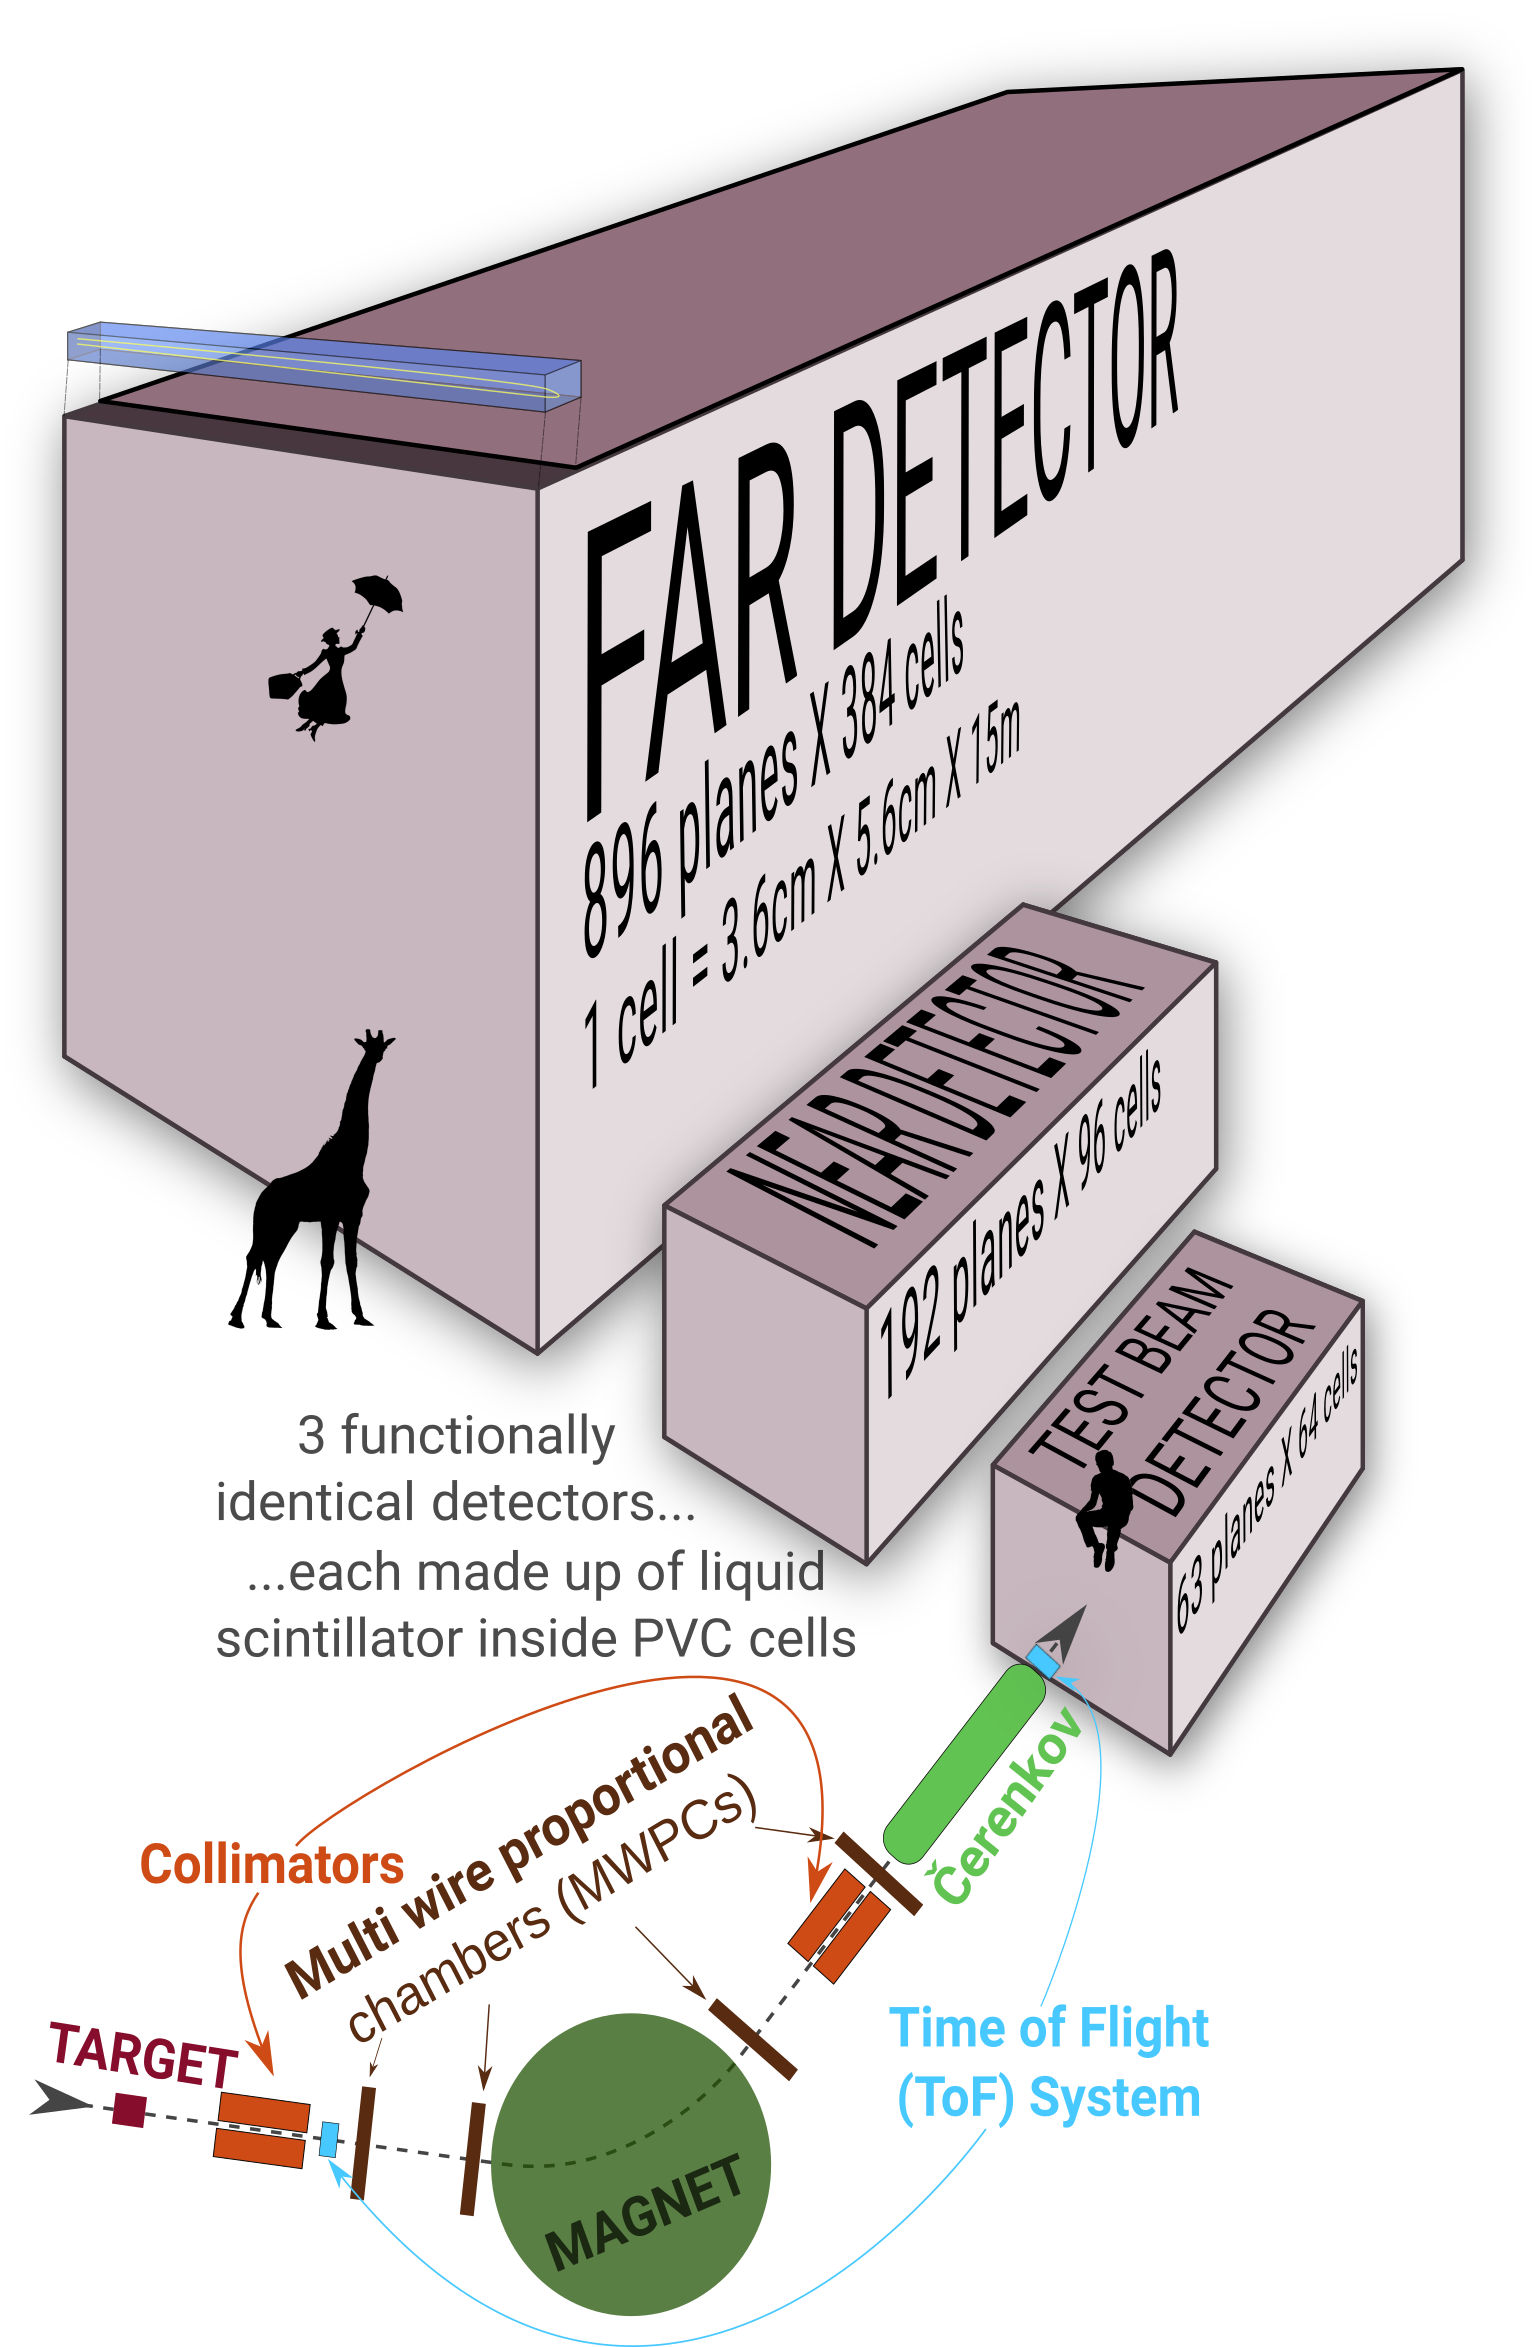
\includegraphics[width=.9\textwidth]{Plots/TestBeamDetectorTextDescription.png}
\caption{Comparison of Test Beam detector scale to other detectors (and a man, giraffe, or Mary Poppins).}
\end{figure}


\subsubsection*{General parameters}
Smaller version of the standard NOvA detectors  made up of 2 vertical and 2 horizontal modules, compared to XxY, or XxY for ND and FD respectively.
" This detector is identical in every way to the Near and Far Detectors but is scaled down, similar to how the Near Detector is a scaled down version of the Far Detector. It consists of 63 planes, and is constructed as a 2x2 module (c.f. ND is 3x3). The total mass is about 30 tons."%[https://cdcvs.fnal.gov/redmine/projects/novatestbeam/wiki/Introduction_to_Test_Beam_for_Analyzers]
63 planes, 32 vertical and 31 horizontal; 64 cells in a plane (2x32 extrusions), readout out in two 32 cell groups;
FD: maxPlane=900, maxCell=390. ND: maxPlane=220, maxCell=100. TB: maxPlane=63, maxCell=64
Detector block taken from NDOS, which had only 31 planes [docdb:28943], beginning and ending with a vertical plane. During comissioning of Test Beam, glued in a horizontal plane in between the two block. [docdb:29543]

%Detector consists of two 31-plane 2x2 blocks + one horizontal plane at FTBF’s MC7 [docdb:33012 (overview of NOvA Test Beam talk)]

Describe the orientation of axes. What's right and left, what's positive and negative w, which planes are vertical and which horizontal (vertical are even starting at 0 and ending in 62 and horizontal are odd).

Readout for the horizontal planes on the opposite side compared to the standard NOvA detectors (why?). Causing underfilled cells in the middle and top of the detector, until... [docdb:49827]
Describe orientation and readout of the TB detector.
Mention the two surveys and the alignment troubles.

\subsubsection*{Scintillator}
Scintillator oil (5600 gallons in total [from Detector Information wiki]) used from ND+NDOS and spare from Texas in the back of the detector (plus some from Ash River afaik).
Block 0 filled with ND+NDOS scintillator oil kept in the tanker [docdb:37152]. Found out the rest of the scintillator in the tanks in Fermilab is contaminated and unusable [docdb:38349] and used NDOS oil from barells to top off horizontal modules.
Shipped scintillator from Ash River and filled the first 21 planes of Block 1 [docdb:41961]. Last 10 planes filled with the NDOS-drained oil from Texas [docdb:34046 describing Texas oil and docdb:41961 showing final filling state].
Maybe show a plot of response at cell centre and mark the 3 different scintillators.

\begin{figure}[hbtp]
\centering
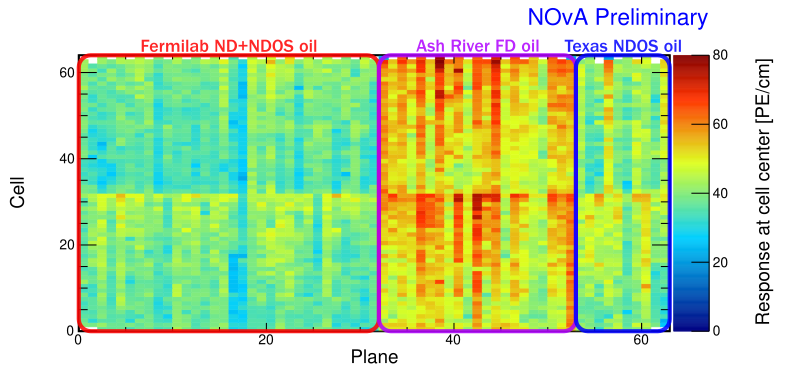
\includegraphics[width=\textwidth]{Plots/TestBeamScintillatorOils.png}
\caption{Uncorrected energy response in the centre of cells across the Test Beam detector showing a clear distinction between the different scintillator oils.}
\end{figure}

\subsubsection*{Readout}
Same readout electronics as in the Far Detector, except for 8 Near Detector Front End Boards, 4 in planes ... (1st quarter of the detector) and another 4 in planes ... (3rd quarter of the detector).
"The Near Detector (ND) and Far Detector (FD) use different versions of the front-end electronics (FEBs, front-end boards), designed to be able to collect data at different rates (the ND is a higher-rate environment than the FD since it is much closer to the beam source). The FD uses FEBv4s (i.e. version 4) and the ND uses FEBv5s. The Test Beam detector uses both in order to be able to make comparisons and validate both versions of the electronics. Most of the FEBs on the Test Beam detector are v4s; of the 126 total, 118 are v4 and 8 are v5."%[https://cdcvs.fnal.gov/redmine/projects/novatestbeam/wiki/Introduction_to_Test_Beam_for_Analyzers]

\subsubsection*{Environment}
Placed in the Fermilab Test Beam Facility with no overburden. Describe environmental controls, temperature dependence etc. Maybe add plots from environmental control (temperature differences etc.) with descriptions of where were the readings taken.

%Main concern is 10 °C dew point (condensaOon in electronics). ND typically runs at 70 °F ± 5 °F. HVAC unit with electric reheat and dew point control, cost of $10.5k, has been received [docdb:3301 - Test Beam overview talk)]

\section{The NOvA calibration process}
Describe the NOvA calibration procedure in general. Describe the benefit of NOvA Test Beam and differences.

Attenutation profiles have a constant binnin fNBins=100 (in w), same for ND, FD and TB. This results in an effectively finer binning for TB compared to ND and FD. For FD w = (-900,+900), ND: (-250,+250), TB: (-150,+150).
TB: 3cm/bin, ND: 5cm/bin, FD: 18cm/bin.
What effect could this have on the relative calibration results? Particularly on the calibration shape?

\subsection{Creating calibration samples}
How do we create the calibration samples and what cuts are applied?

\begin{figure}[hbtp]
\centering
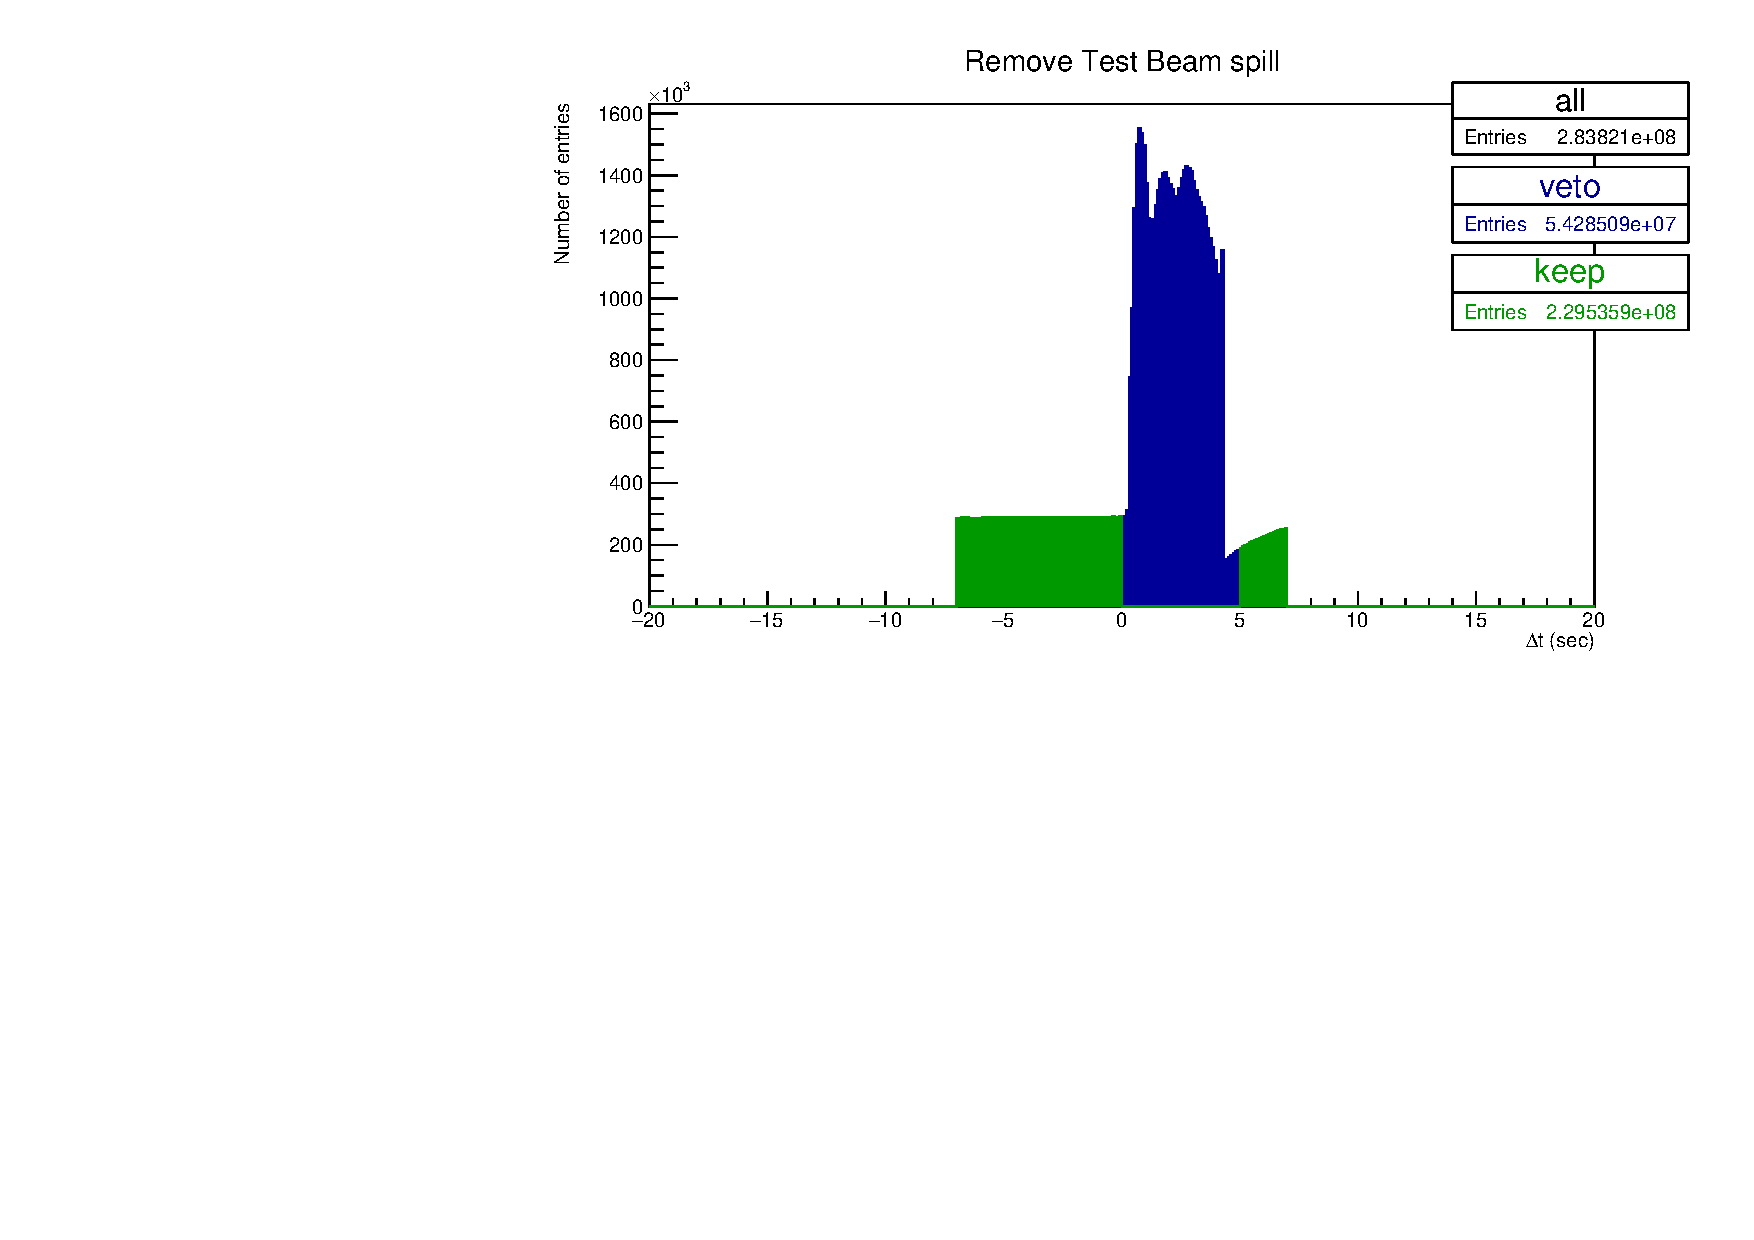
\includegraphics[width=\textwidth]{Plots/RemoveTBSpills.pdf}
\caption{Test Beam beam spill events removed from the calibration samples. Test Beam beam spill is 4.2 seconds long and we remove events (in blue) within a 5 seconds window from the start of the beam spill. The remaining events (green) should mostly consist of cosmic particles. This example and the numbers of entries are for the full period 4 Test Beam sample.}
\end{figure}


\subsubsection*{Tricell condition}
\begin{figure}[hbtp]
\centering
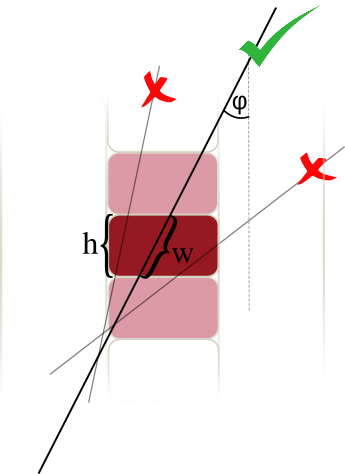
\includegraphics[width=0.25\textwidth]{Plots/TricellConditionWithDescription.png}
\caption{Illustration of the tricell condition. We only use hits that have two surrounding hits in the same plane to be used in the NOvA calibration. This is to ensure a good quality of the pathlength (w) reconstruction, which is calculated from the known cell height (h) and the reconstructed track angle $\left(\varphi\right)$.}
\end{figure}


\begin{figure}[hbtp]
\centering
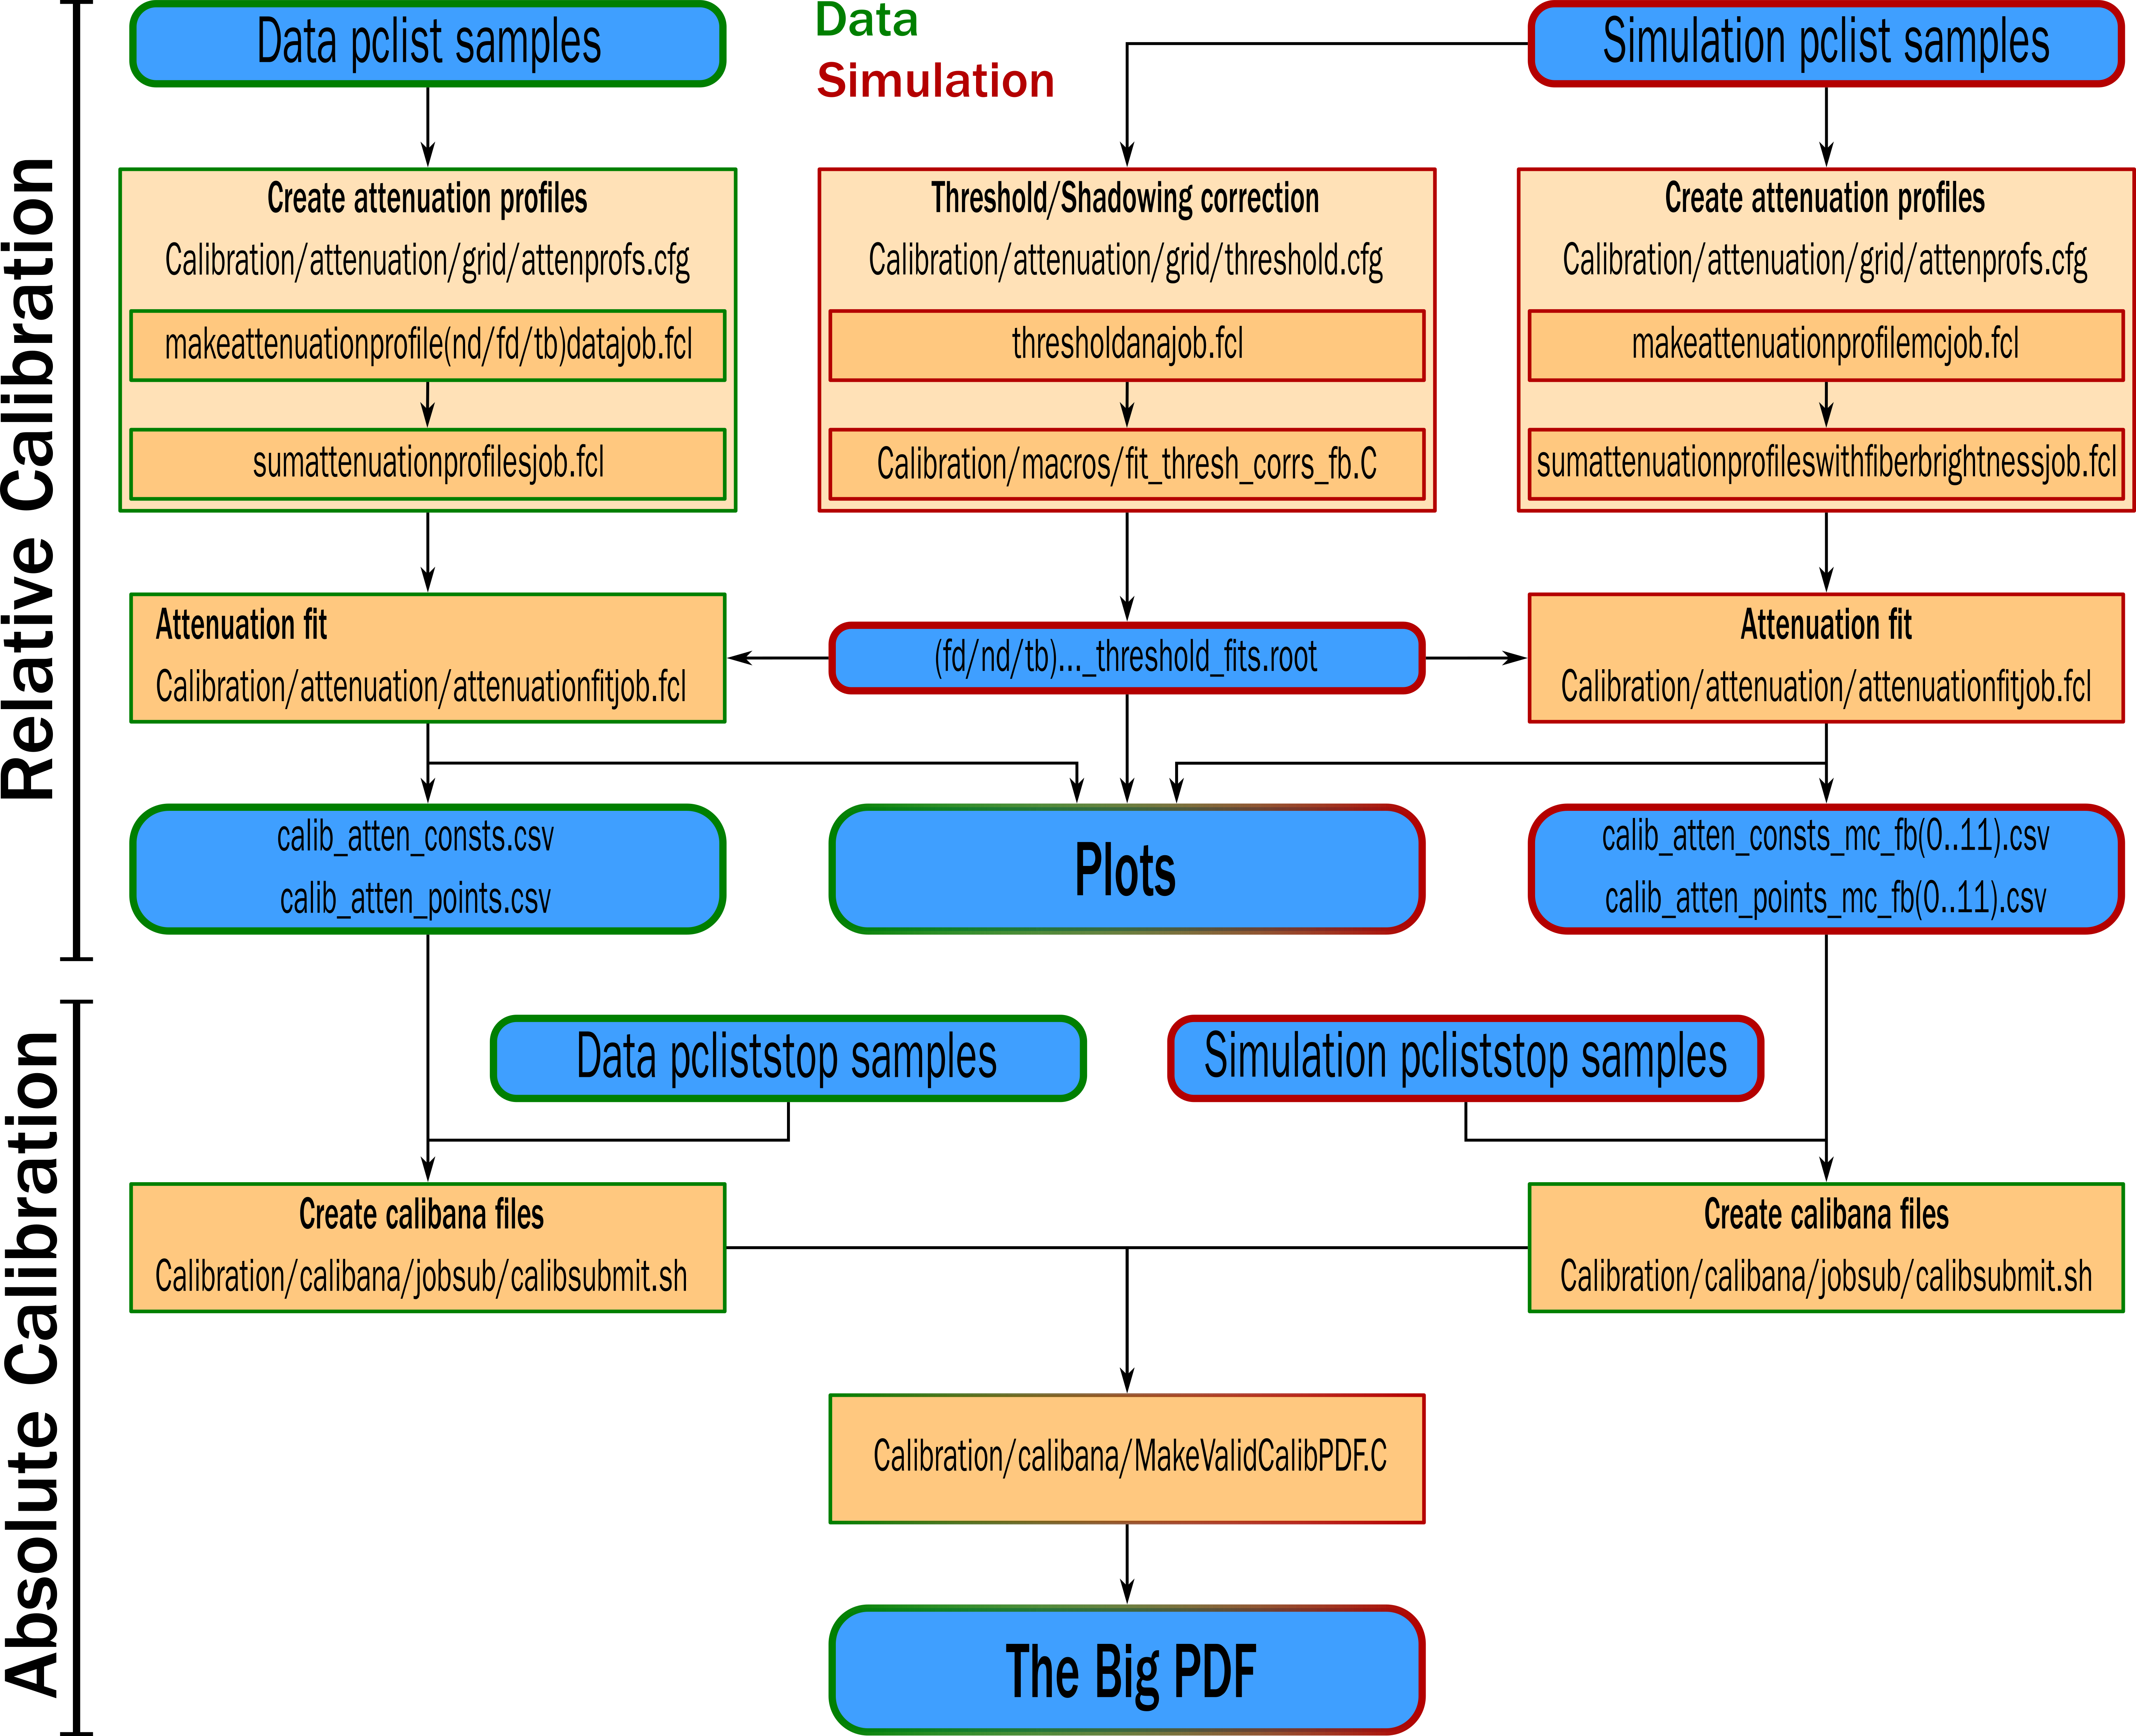
\includegraphics[width=\textwidth]{Plots/CalibrationFlowChart.png}
\caption{Flow chart showing the jobs (orange background) and files (blue background) needed and produced during the full NOvA calibration process. The left chain is showing the data calibration process (with green border) and is applied to every data calibration sample separately (periods or epochs). The center and right chains are showing the simulation calibration proces, which is redone only if there's a change to the detector simulation. The absolute calibration at the bottom combines data and simulation. The entire process is done separately for each NOvA detector.} 
\end{figure}

\subsection{Calibration uncertainties}

\section{NOvA Test Beam detector calibration}
\subsection{Overview}
History of TB calibration. What led to the final version of TB calibration. What can be done next.



Dates and times when the data taking occured.

Period naming, possibly epochs (for P3).
List of data samples, plus MC samples that were used and pointer to the data-based simulation technote.
%Possibly refer to https://cdcvs.fnal.gov/redmine/projects/novatestbeam/wiki/Period_and_Epoch_Naming

Specific running conditions:
Underfilled cells
Faulty FEBs (Period 2 and Period 3)
Why do we do the calibration generally and why do we need to do in for Test Beam specifically

Temperature study (small overview)

\subsubsection{Definitions}
List all final data and simulation definitions used.

\subsection{Detector Brightness}

\begin{figure}[hbtp]
\centering
\begin{subfigure}[b]{0.495\textwidth}
\centering
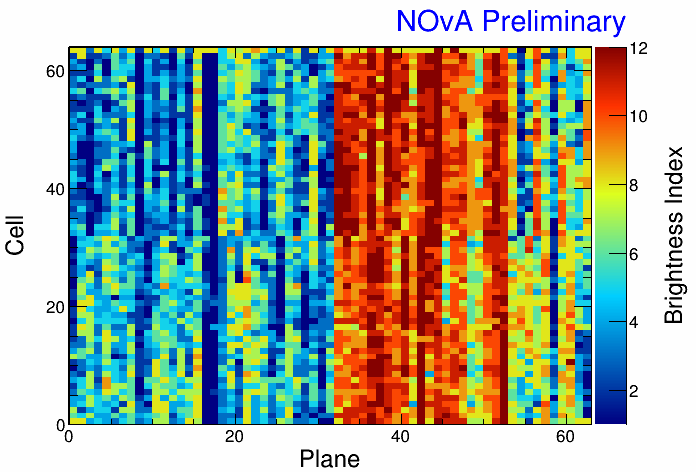
\includegraphics[width=\textwidth]{Plots/BrightnessIndex.png}
\end{subfigure}
%\hfill
\begin{subfigure}[b]{0.495\textwidth}
\centering
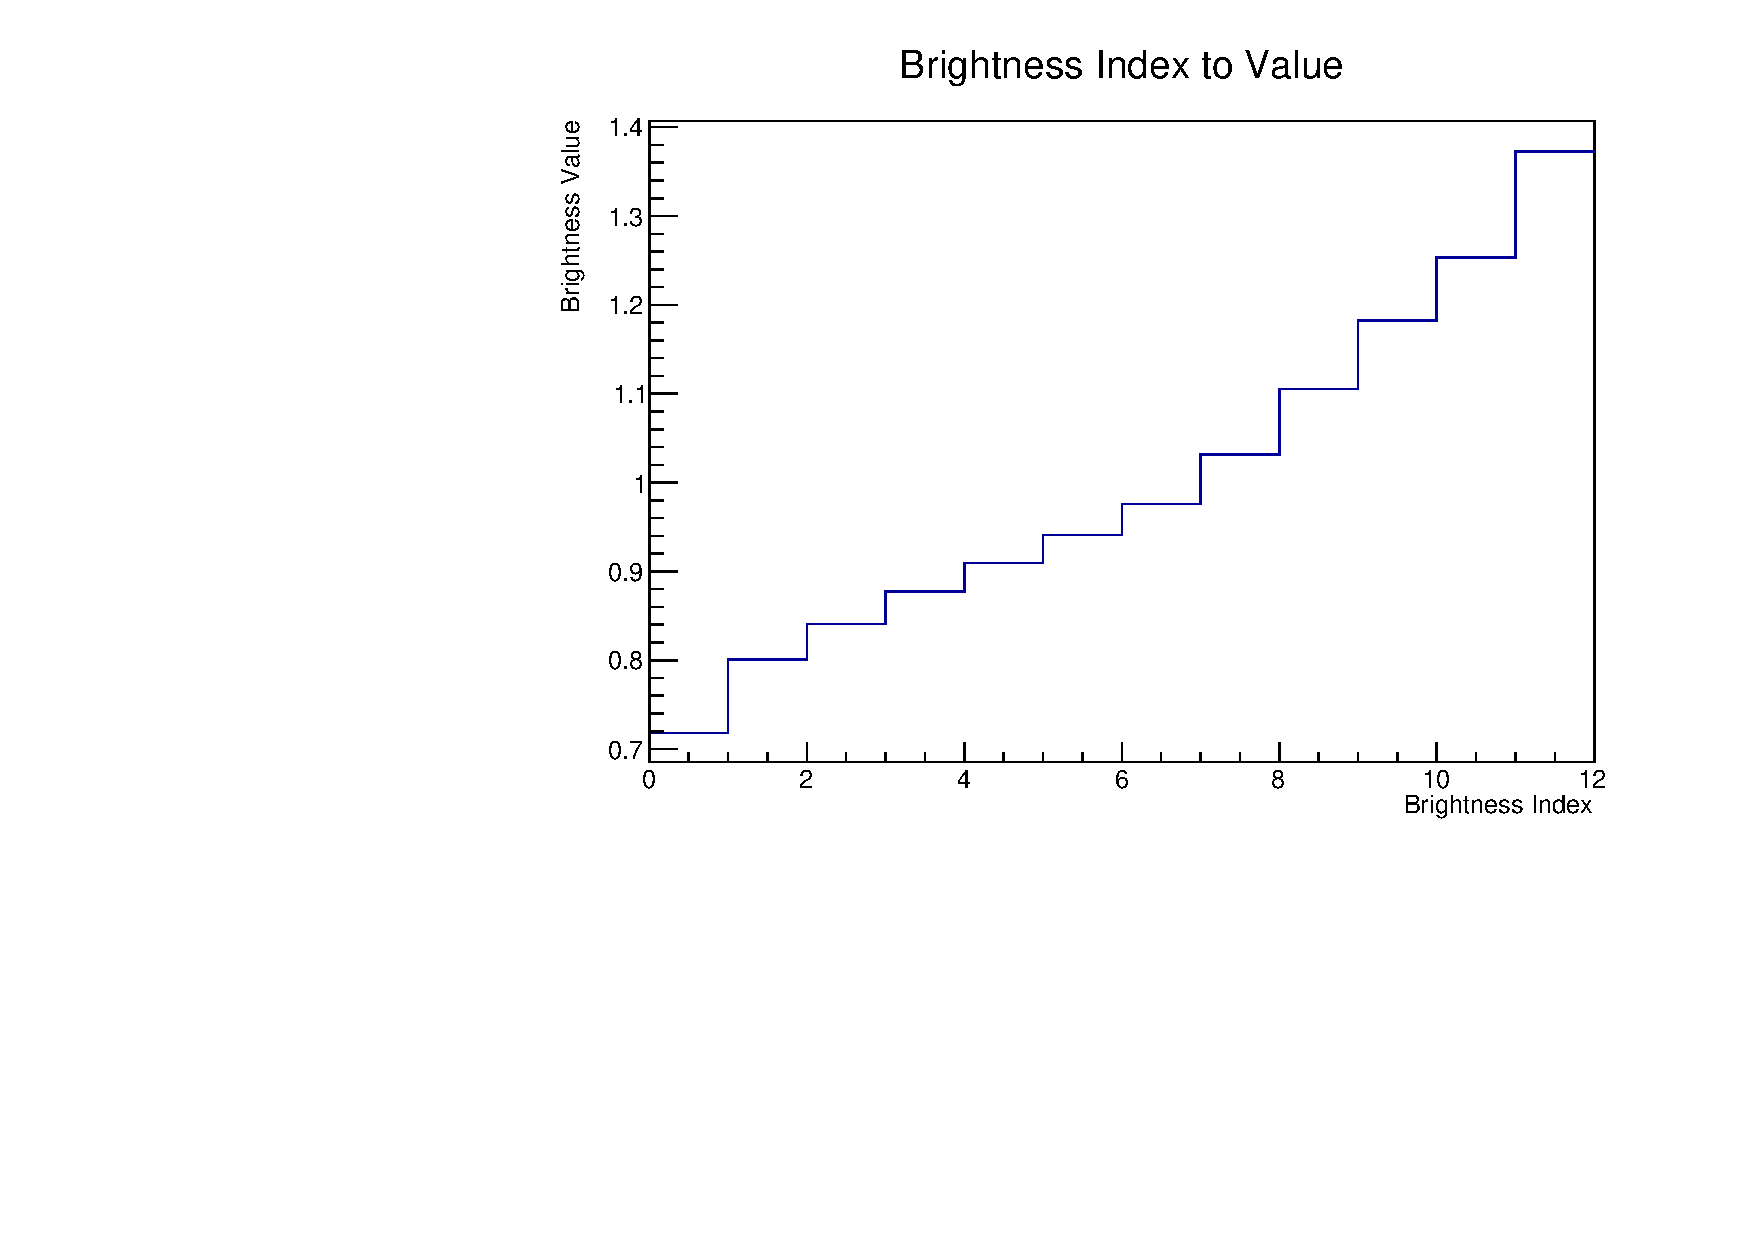
\includegraphics[width=\textwidth]{Plots/BrightnessIndexToValue.pdf}
\end{subfigure}
\caption{The Test Beam detector is (like the standard NOvA detectors) divided into 12 brightness bins (left plot), each representing a relative difference in energy response (right plot) due to different brightnesses of the fibers, scintillators, or readout.}
\end{figure}

\subsection{Simulation}

We originally used Teresa's calibration MC sample, but after we saw disagreement, we developed a new MC based off of the period 3 data, which we ended up using for both period 2 and period 3. For fibre brightness we are also using the same MC from period 3 data as it represents the detector in its best condition.

We used a data-based simulation of cosmic muons for the Test Beam detector calibration. The details are described in the technote XXX. We used this and this data as a basis and this and this data for the fiber brighness file.

\begin{figure}[!hbtp]
\centering
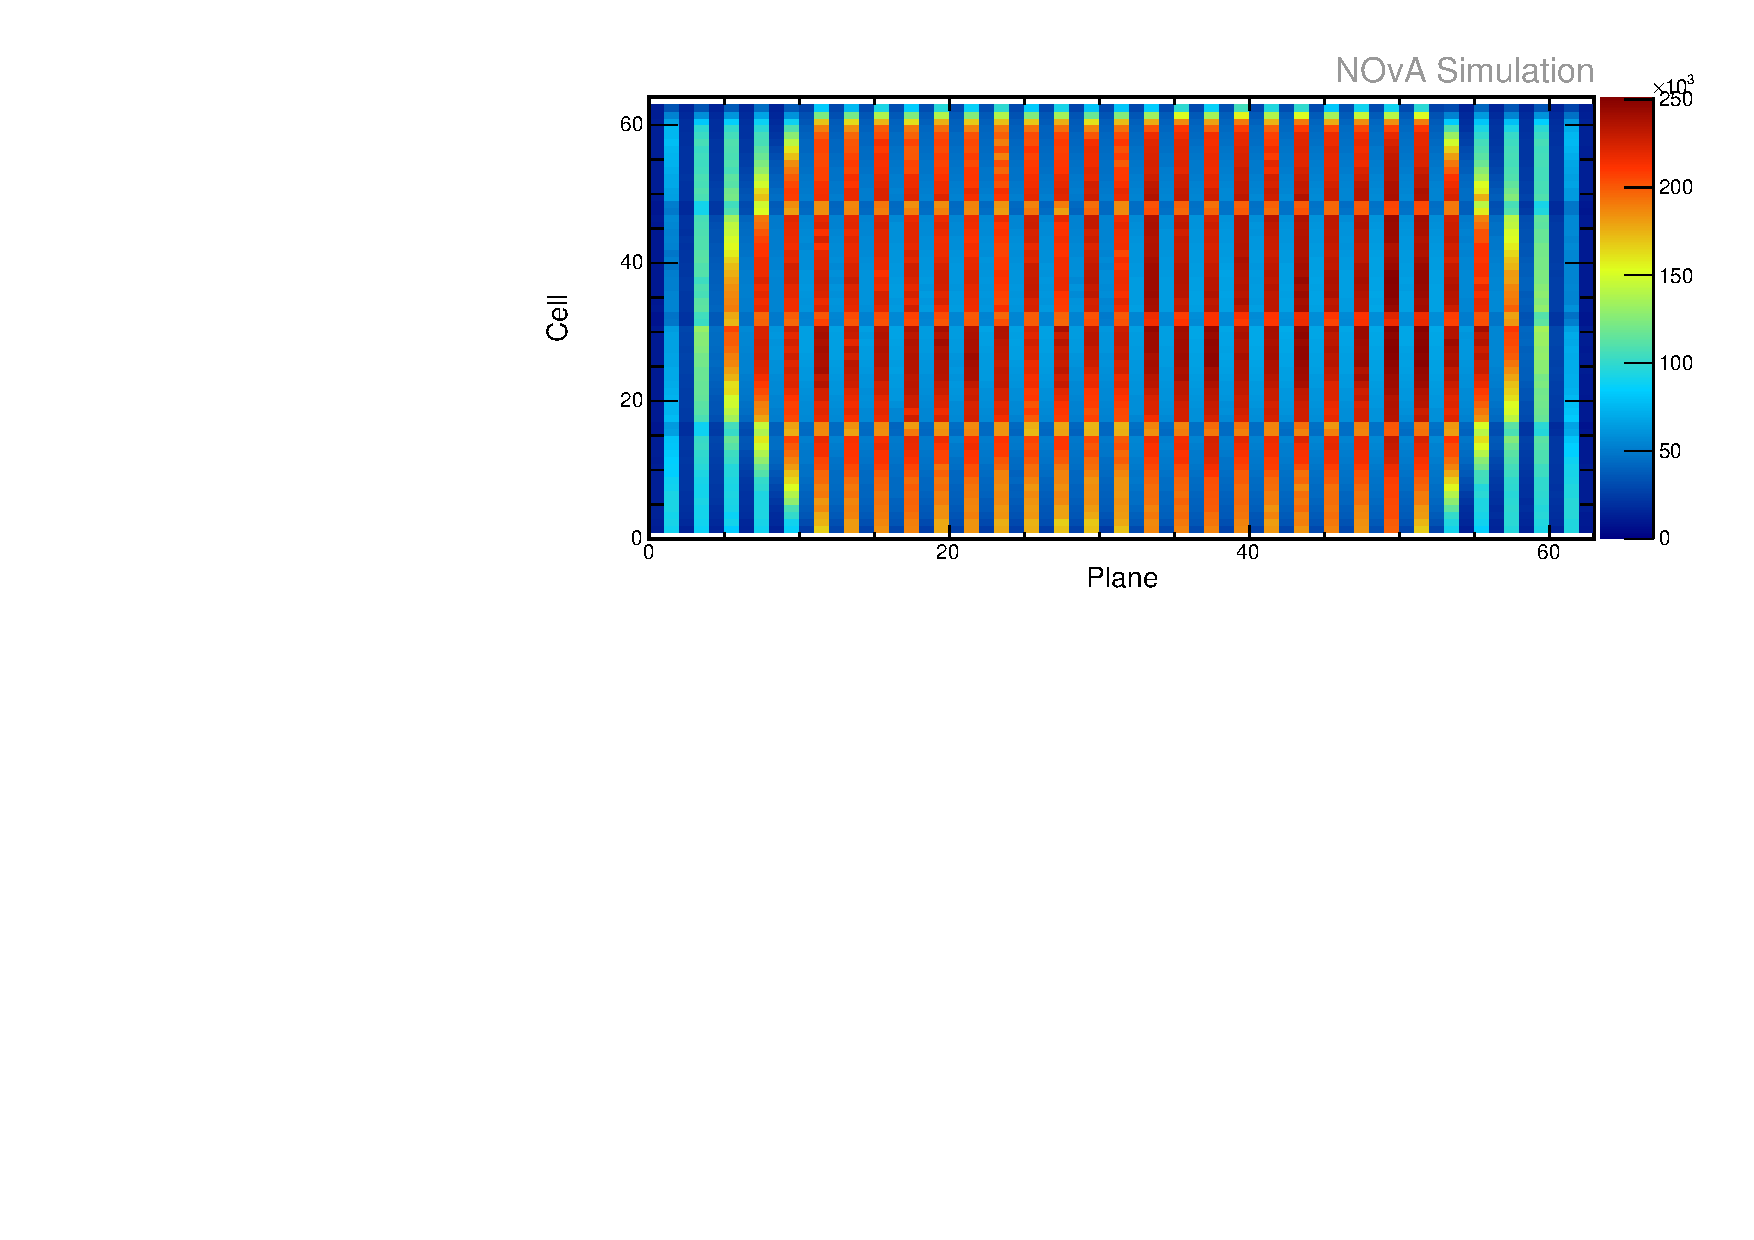
\includegraphics[width=\textwidth]{Plots/Attenprofs_Simulation_CellPlane.pdf}
\caption{Distribution of events in the Test Beam simulation calibration sample.}
\end{figure}

\subsubsection{Relative calibration results}
\begin{figure}[!hbtp]
\centering
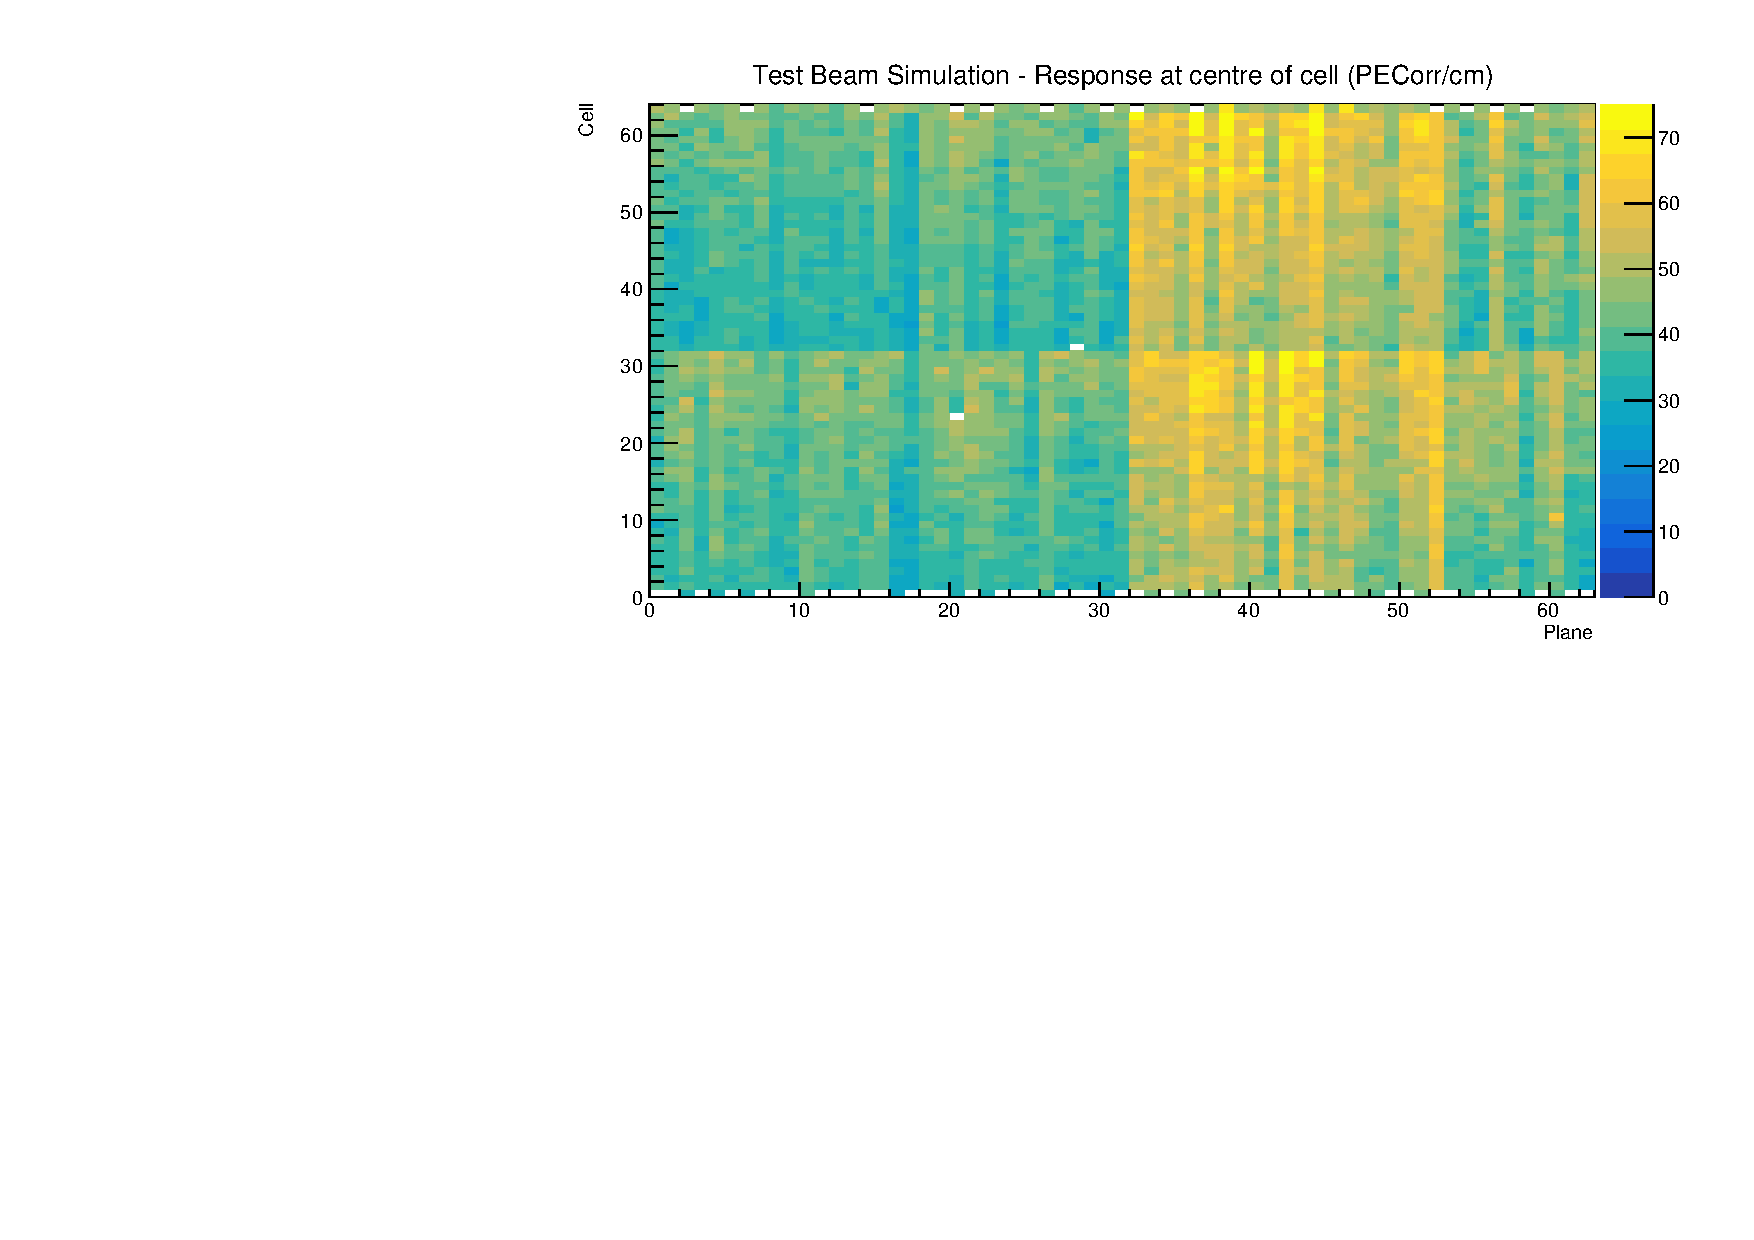
\includegraphics[width=\textwidth]{Plots/CellResponseAtCentre_Prod4DataBasedSim.pdf}
\caption{Overview of the relative calibration results for the Teast Beam detector simulation. Each cell is represents the average corrected energy response (in PECorr/cm) in the centre of each cell. The blank cells are uncalibrated.}
\end{figure}

\subsection{Period 1}
Only a month of data, only first half of detector filled, primary/secondary beam halo, or oversaturation leading to FEB shutoffs [docdb:38349 and 41331].
Only used for comissioning, not used for any data analysis or calibration.

\subsection{Period 2}
What was done for the period 2 tb calibration, short overview of what has been done: test beam data were calibrated all at the same time without splitting them to separate epochs. See figures \ref{figCalibhistWPE_period2},\ref{figCalibhistCellPE_period2} and \ref{figCalibhistPlanePE_period2}.

\begin{figure}[!hbtp]
\centering
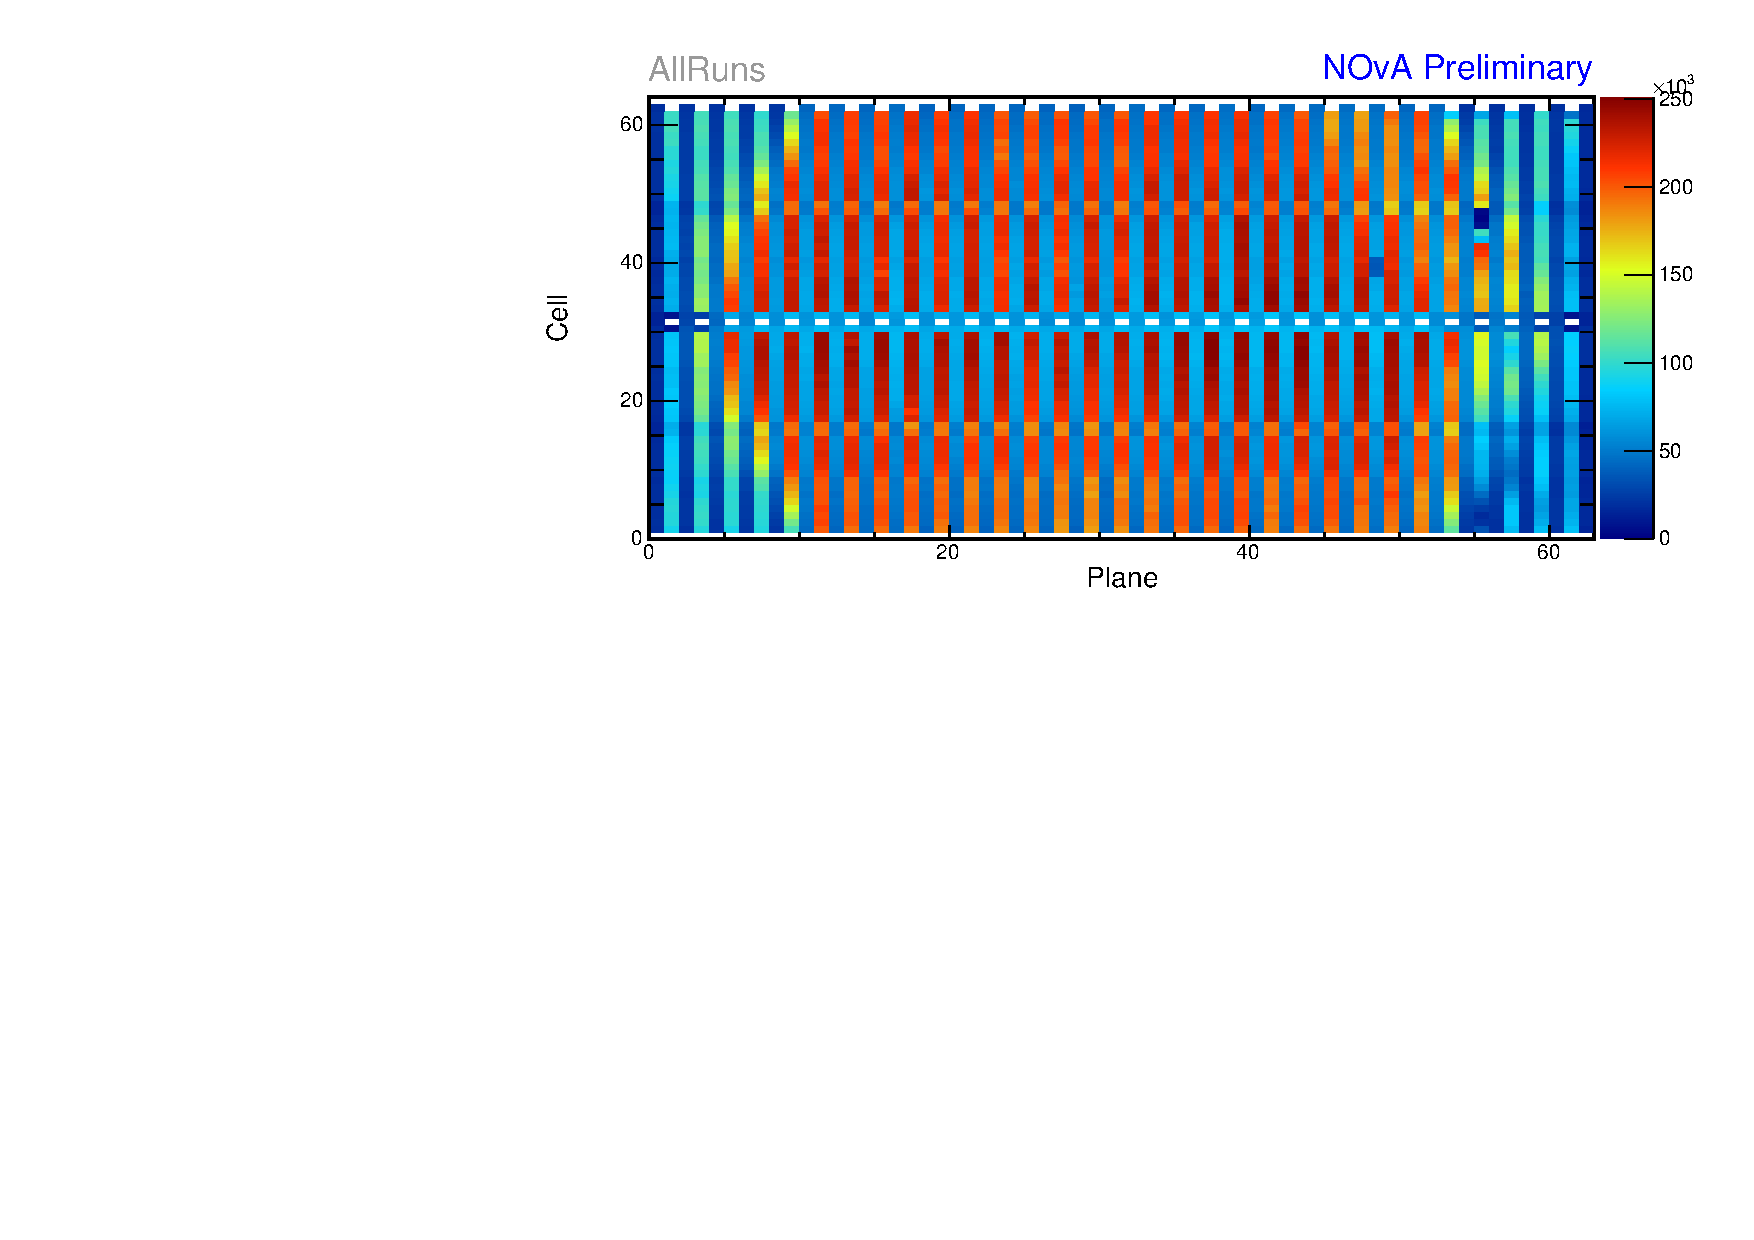
\includegraphics[width=\textwidth]{Plots/Attenprofs_P2Data_CellPlane_AllRuns.pdf}
\caption{Distribution of events in the period 2 Test Beam data calibration sample.}
\end{figure}

\begin{figure}[!hbtp]
\centering
\begin{subfigure}[b]{\textwidth}
\centering
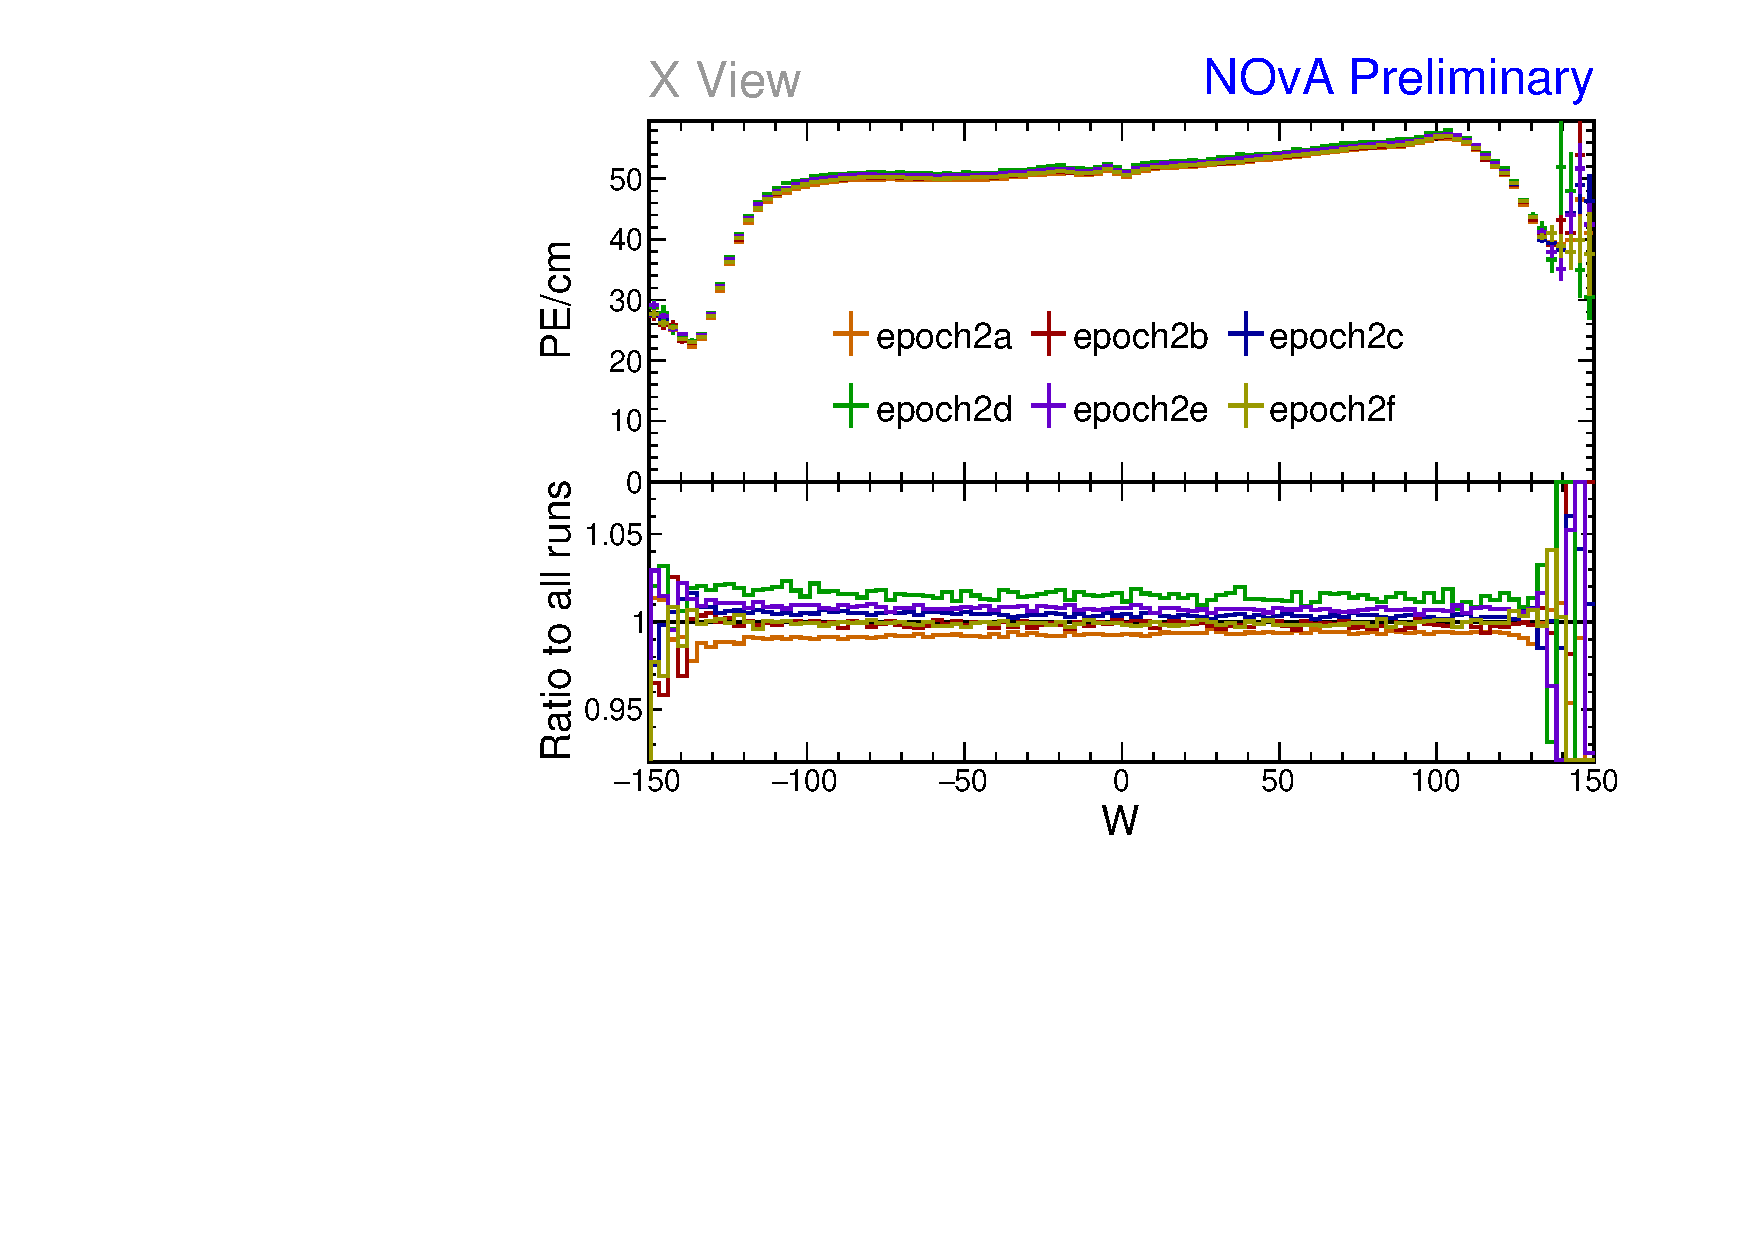
\includegraphics[width=\textwidth]{Plots/Attenprofs_P2Data_WPE_corr_xy_X_Combined.pdf}
\end{subfigure}
\begin{subfigure}[b]{\textwidth}
\centering
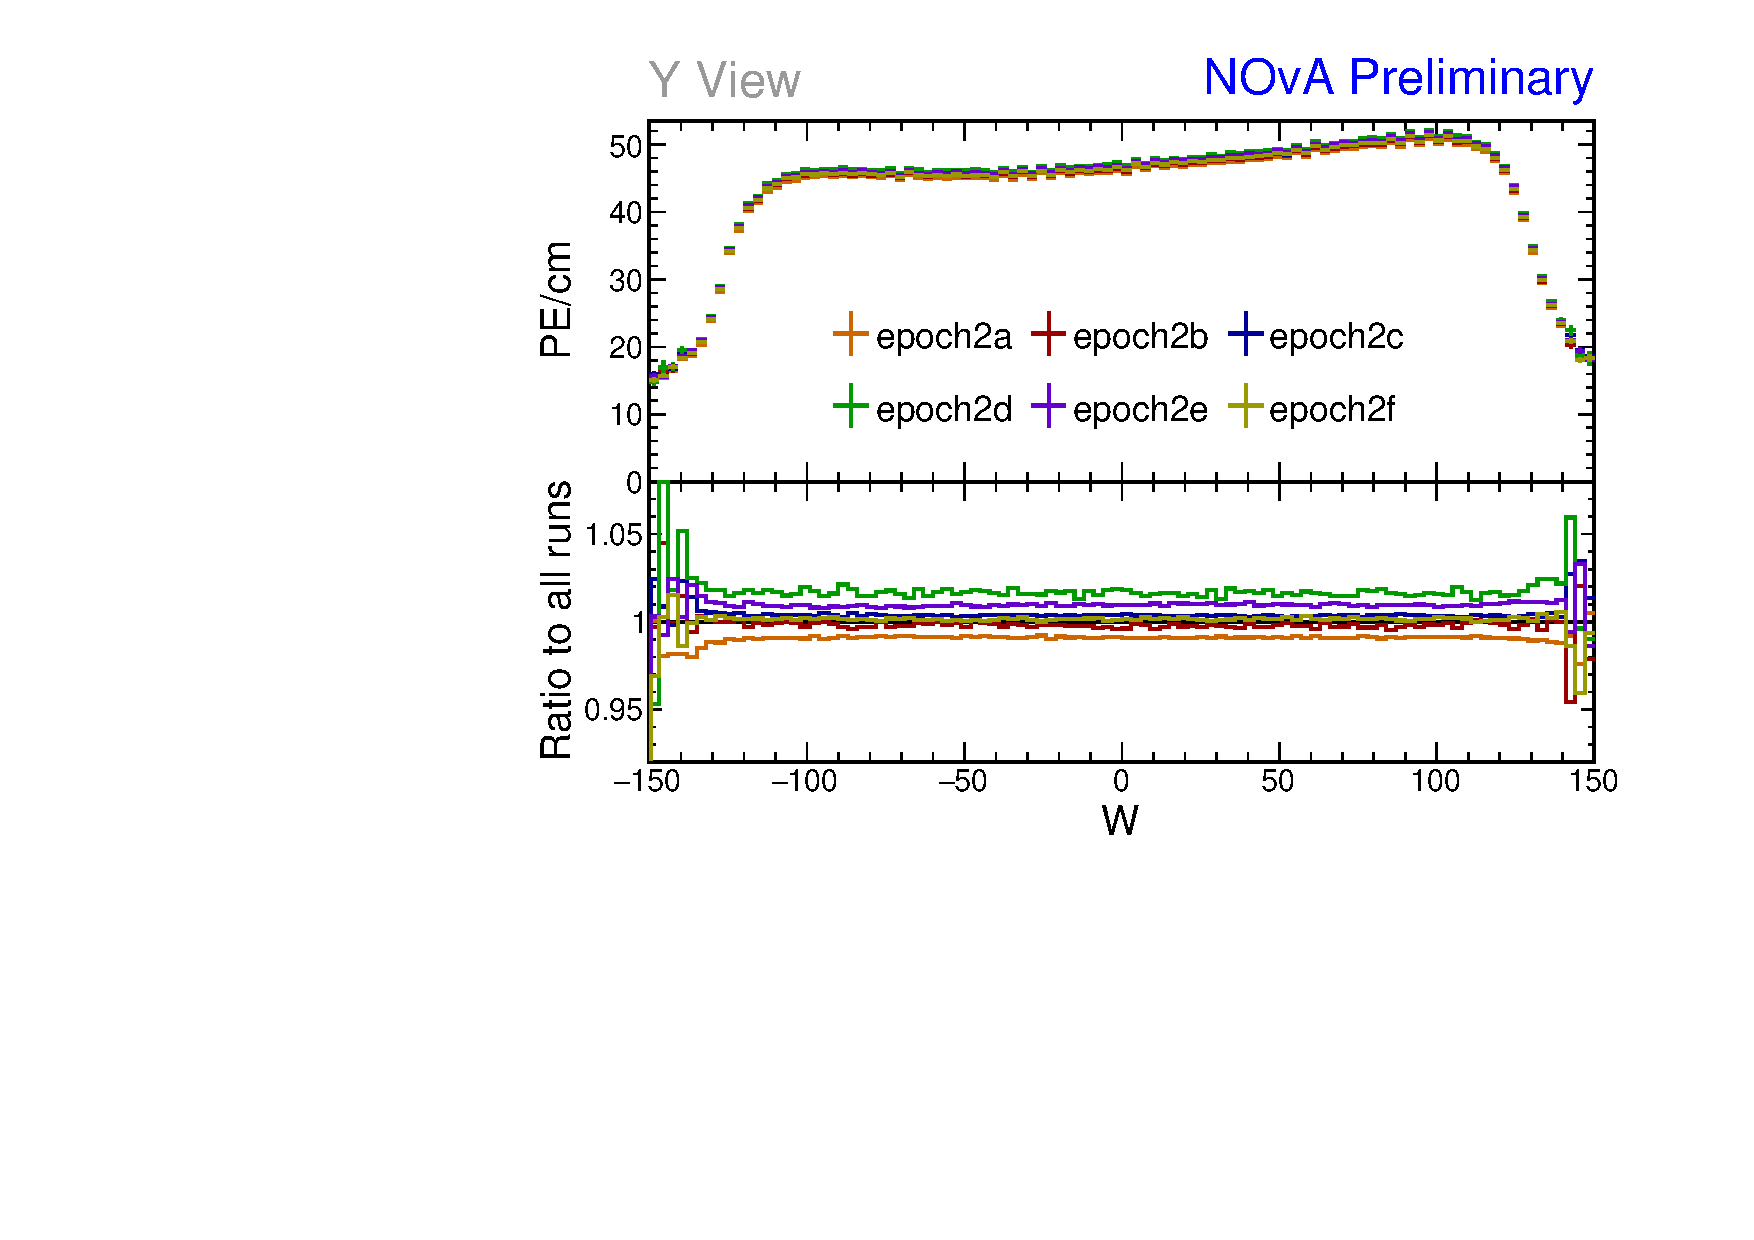
\includegraphics[width=\textwidth]{Plots/Attenprofs_P2Data_WPE_corr_xy_Y_Combined.pdf}
\end{subfigure}
\caption{Uncorrected average energy response as a function of the position within a cell (w) for epochs in period 2. It is clear that there is no significant difference between the various epochs.}
\label{figCalibhistWPE_period2}
\end{figure}

\begin{figure}[!hbtp]
\centering
\begin{subfigure}[b]{\textwidth}
\centering
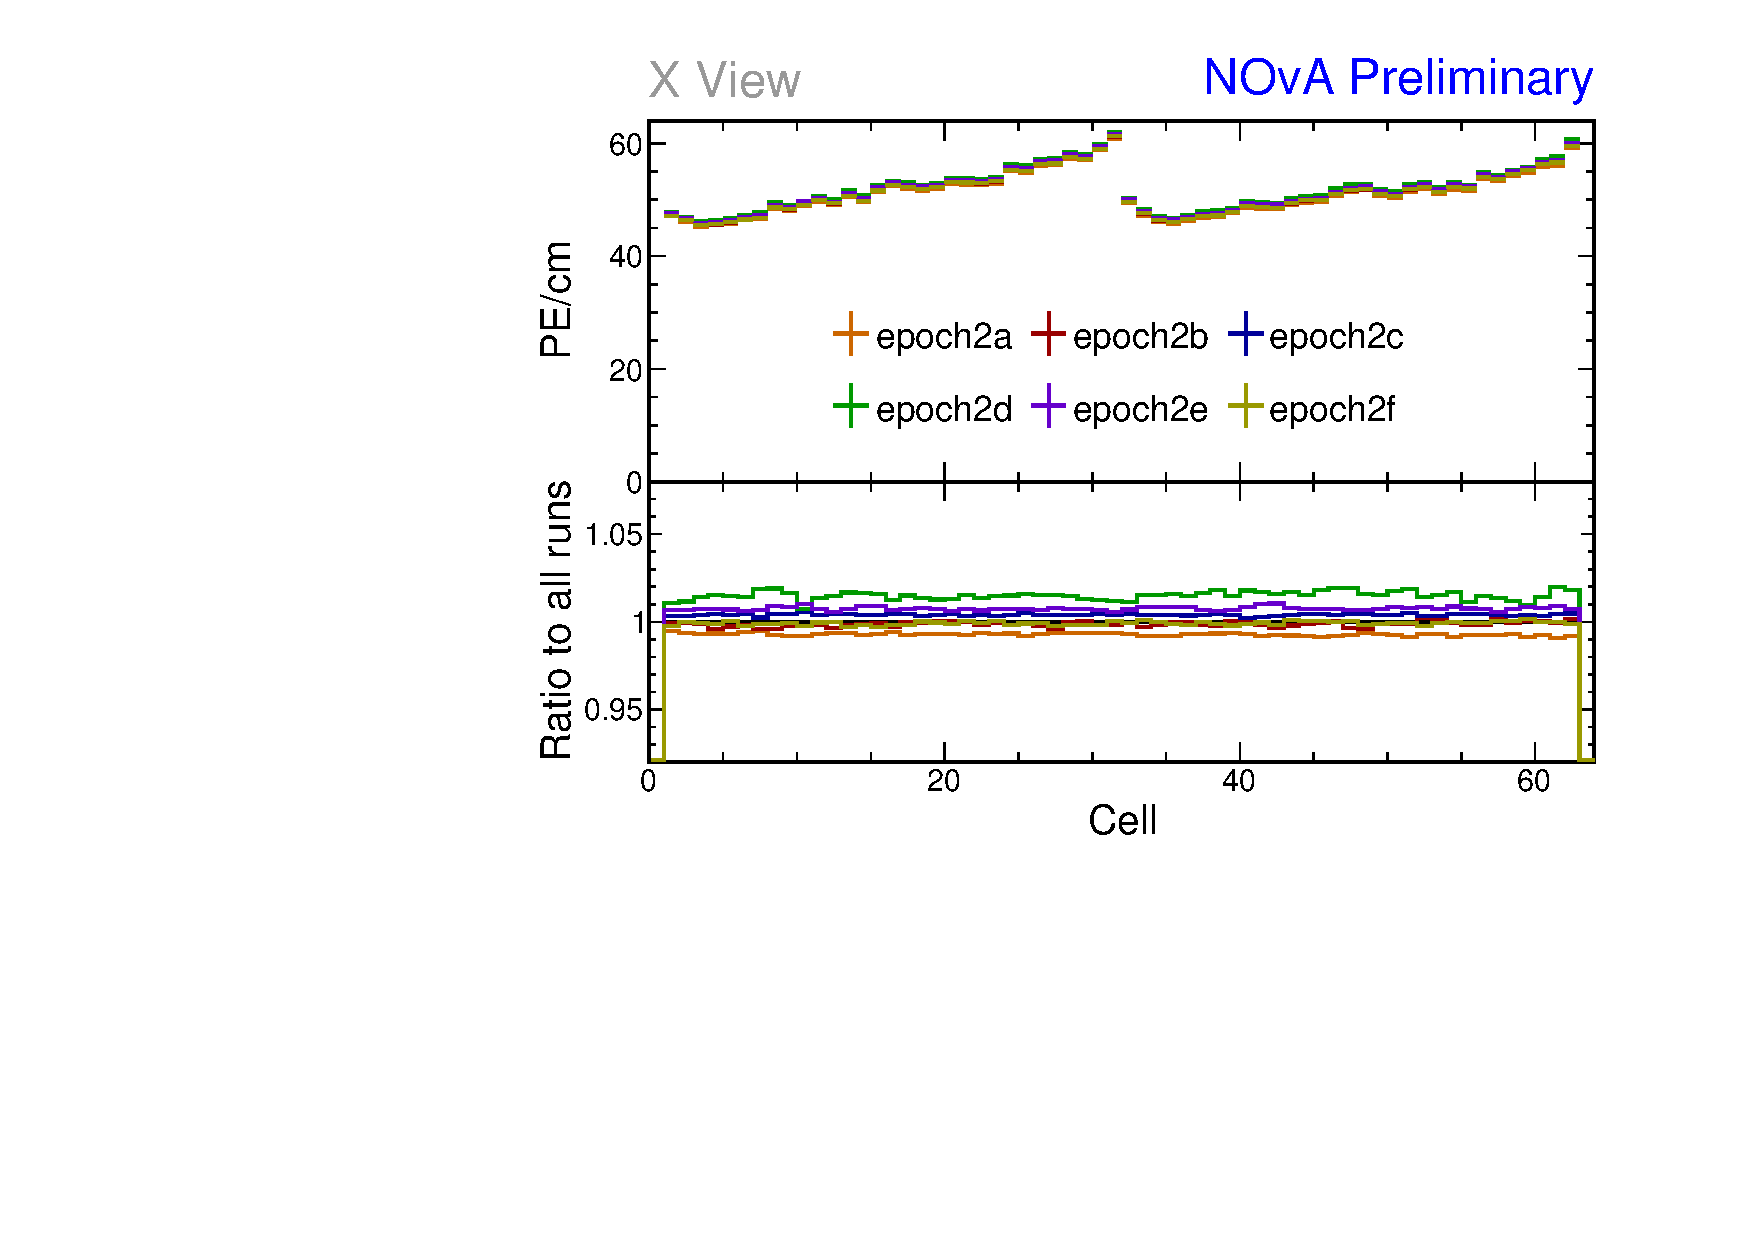
\includegraphics[width=\textwidth]{Plots/Attenprofs_P2Data_CellPE_X_Combined.pdf}
\end{subfigure}
\begin{subfigure}[b]{\textwidth}
\centering
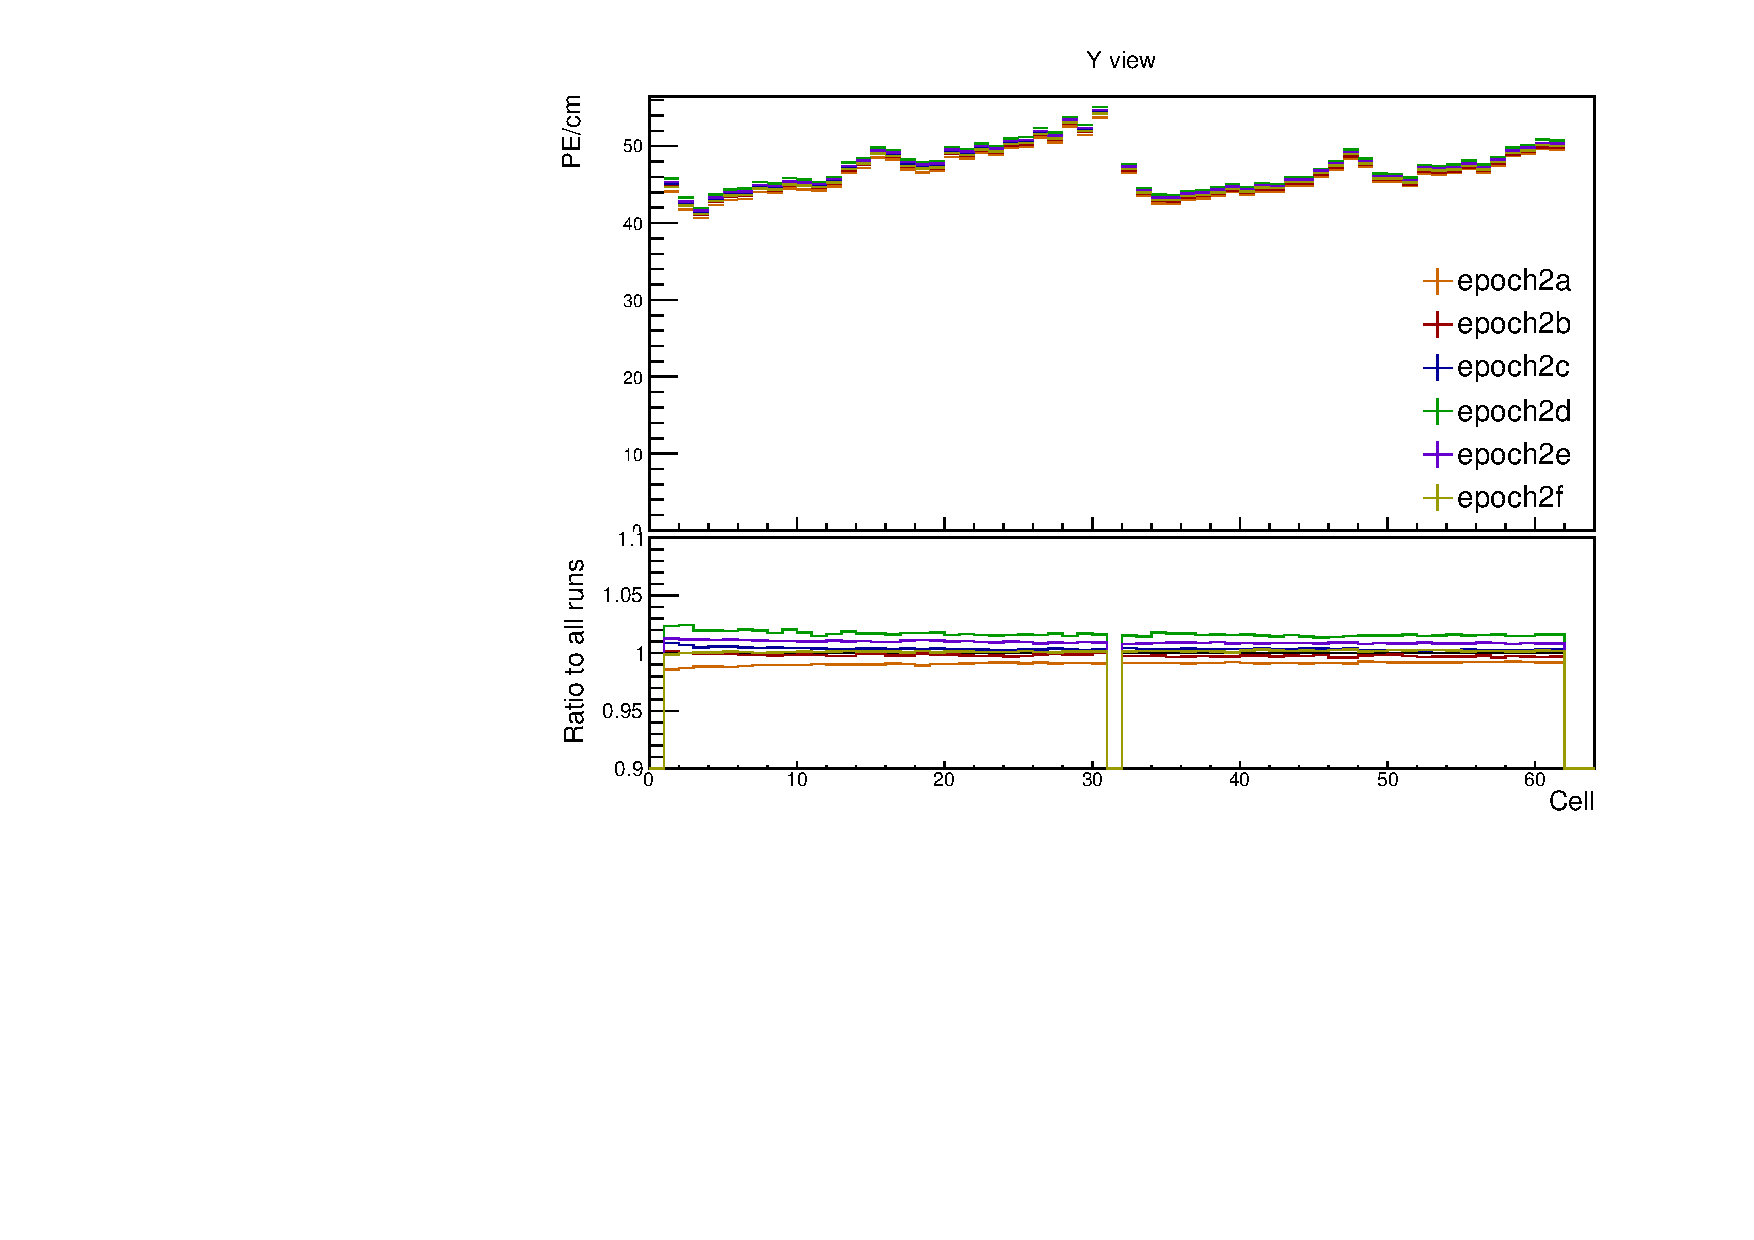
\includegraphics[width=\textwidth]{Plots/Attenprofs_P2Data_CellPE_Y_Combined.pdf}
\end{subfigure}
\caption{Uncorrected average energy response as a function of cells for epochs in period 2.}
\label{figCalibhistCellPE_period2}
\end{figure}

\begin{figure}[!hbtp]
\centering
\begin{subfigure}[b]{\textwidth}
\centering
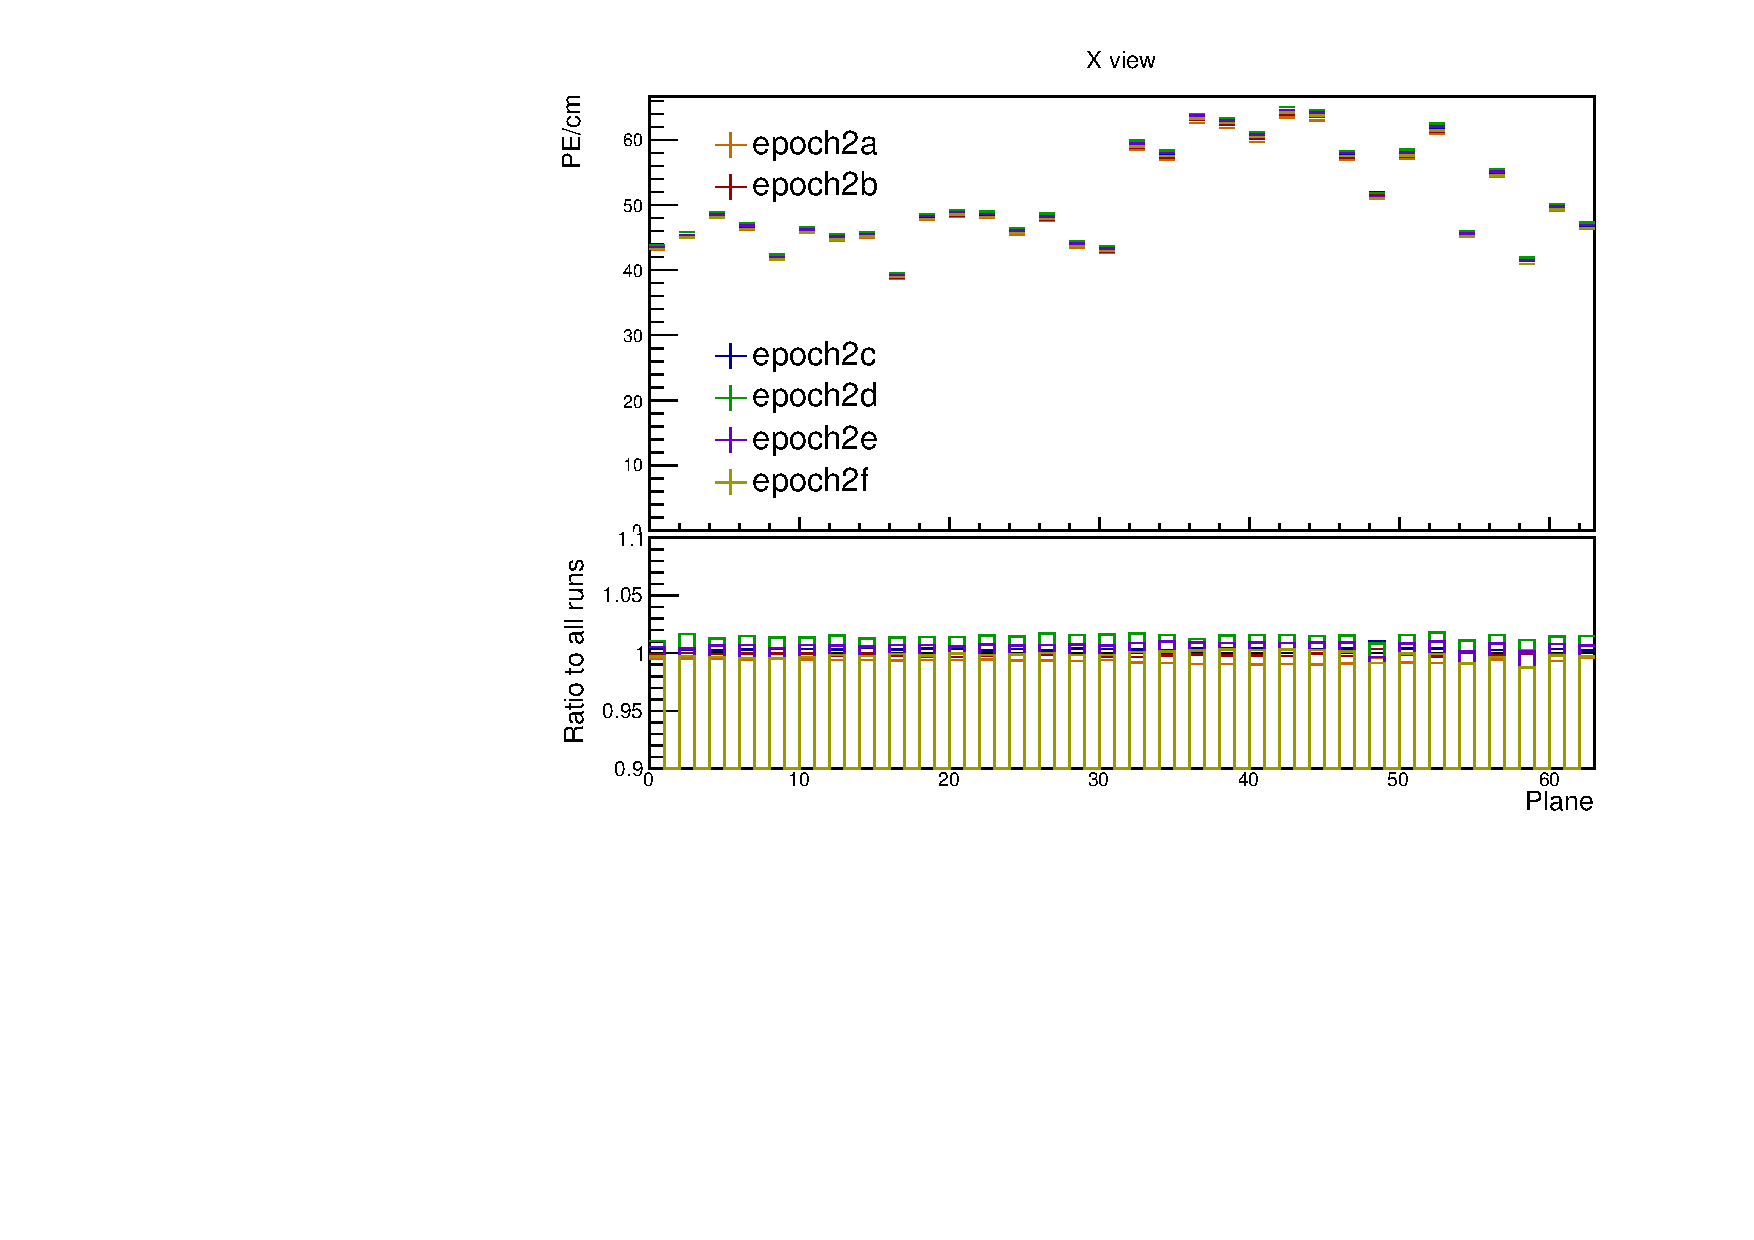
\includegraphics[width=\textwidth]{Plots/Attenprofs_P2Data_PlanePE_X_Combined.pdf}
\end{subfigure}
\begin{subfigure}[b]{\textwidth}
\centering
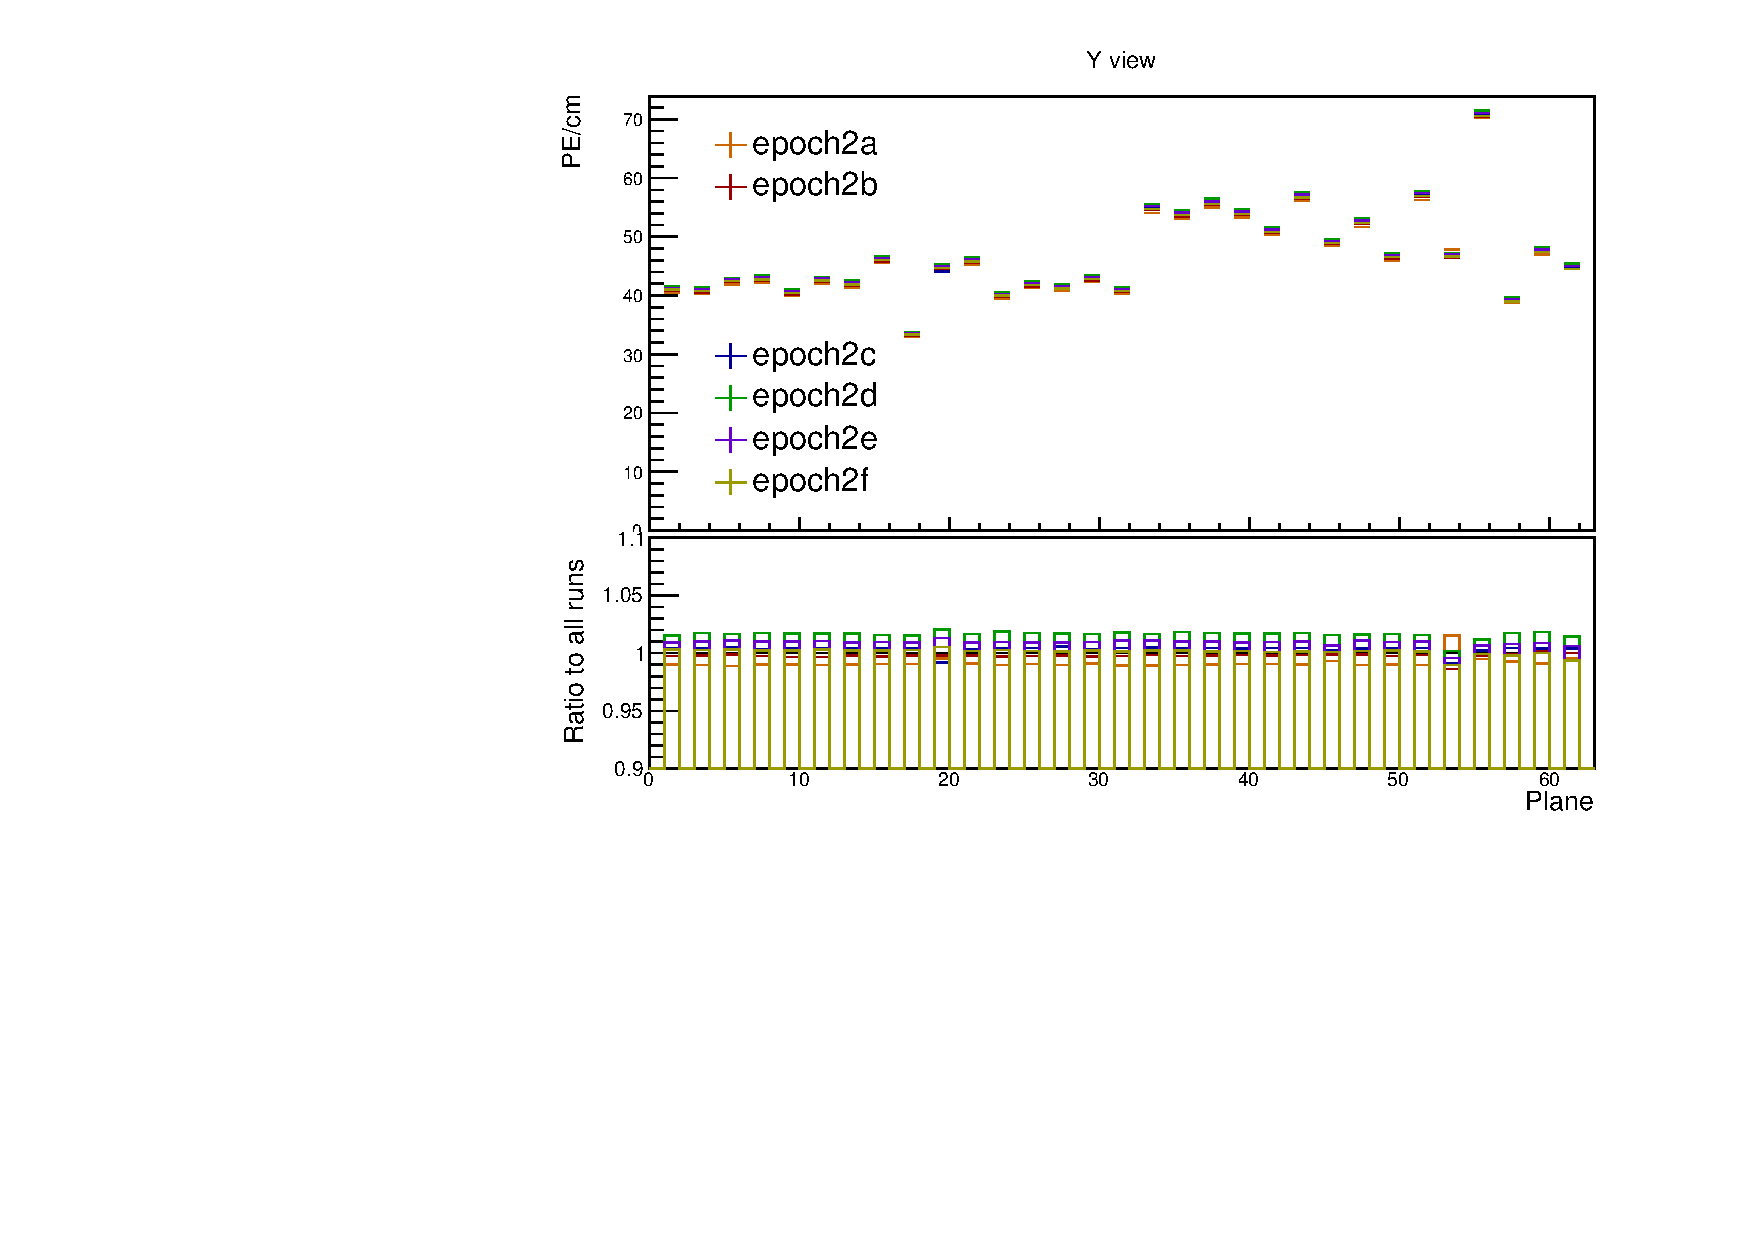
\includegraphics[width=\textwidth]{Plots/Attenprofs_P2Data_PlanePE_Y_Combined.pdf}
\end{subfigure}
\caption{Uncorrected average energy response as a function of planes for epochs in period 2.}
\label{figCalibhistPlanePE_period2}
\end{figure}

\subsubsection{Relative calibration results}

\begin{figure}[!hbtp]
\centering
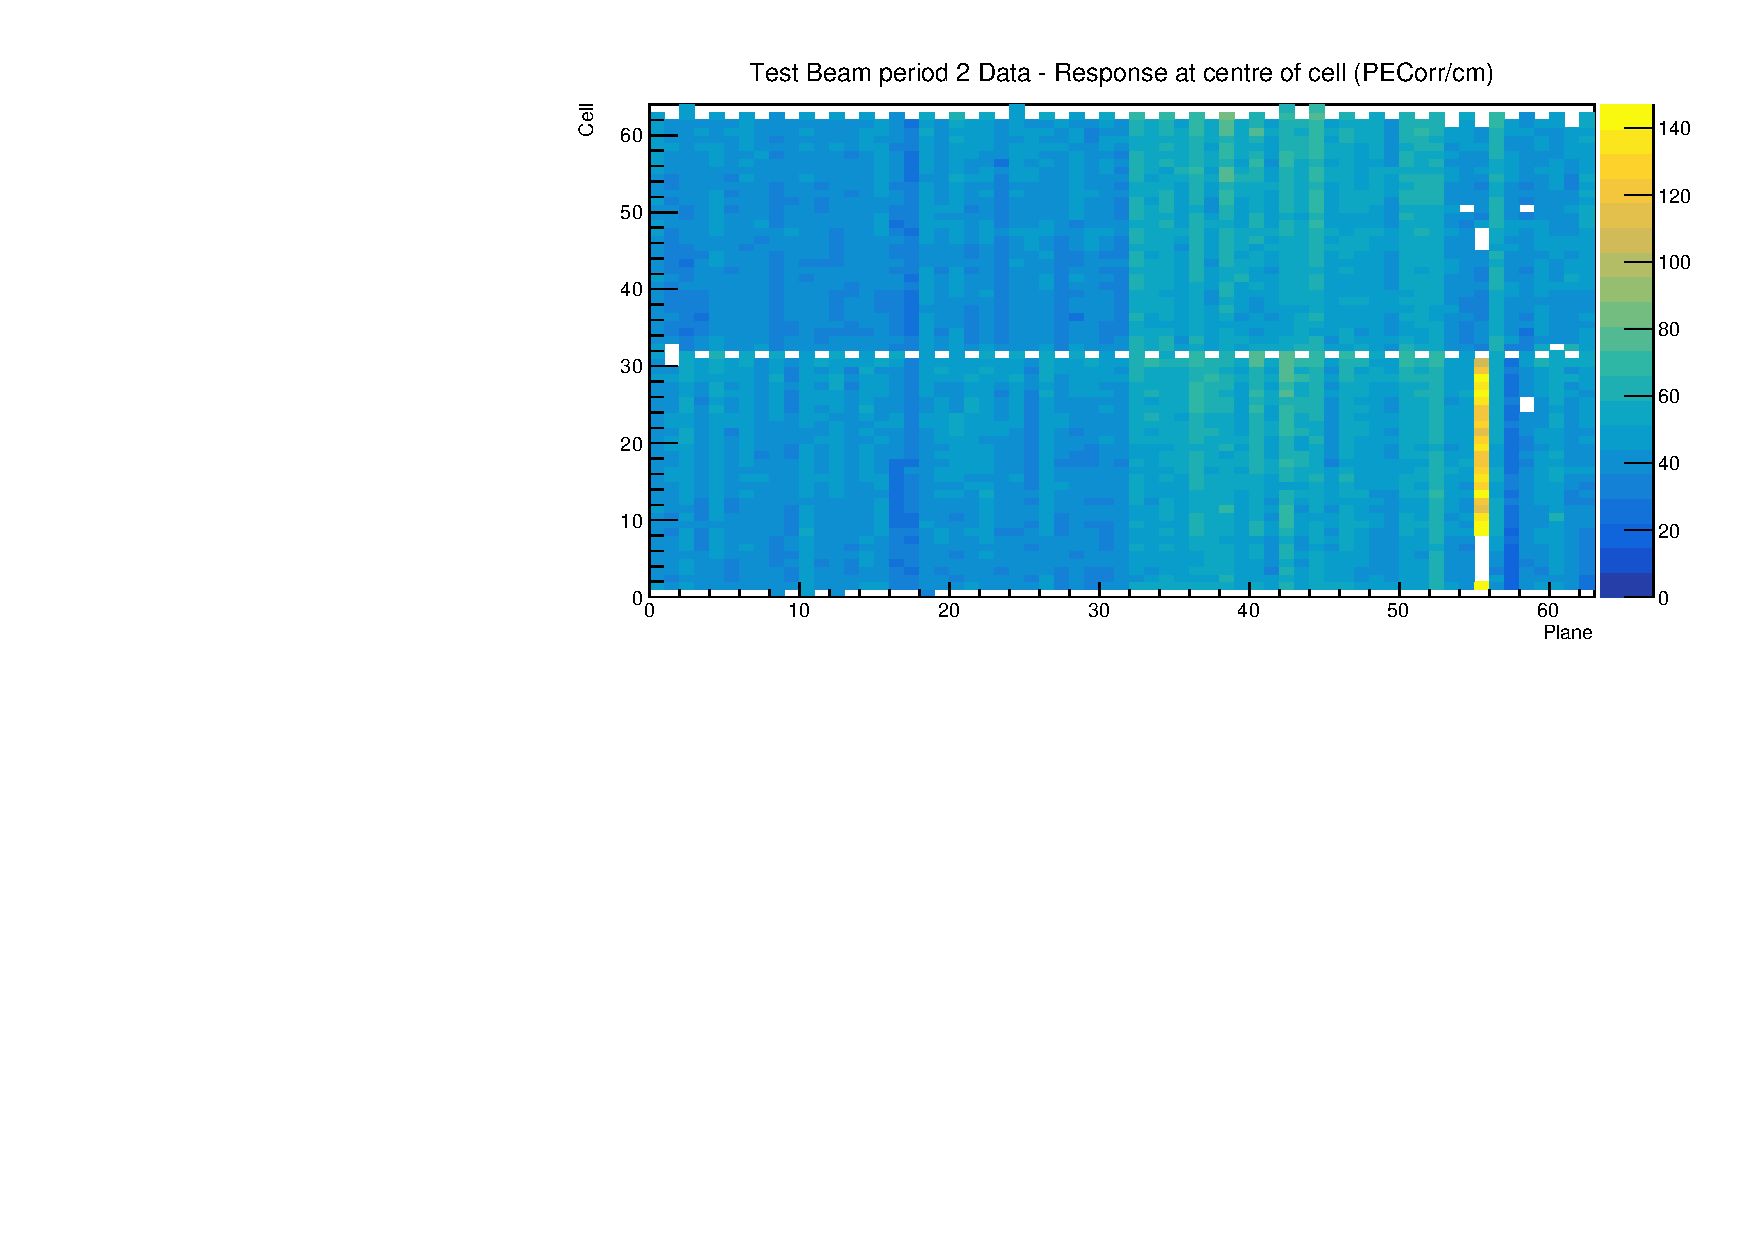
\includegraphics[width=\textwidth]{Plots/CellResponseAtCentre_period2.pdf}
\caption{Overview of the relative calibration results for the Teast Beam detector period 2 data. Each cell is represents the average corrected energy response (in PECorr/cm) in the centre of each cell. The blank cells are uncalibrated.}
\end{figure}

\subsection{Period 3}
Separation of Period 3 data into different epochs based on the running conditions (include plot of the running conditions). We are separating data into pre- and post- filling states. We're using only the fully-refilled post-FEB swap data from period 3 as a basis for the simulation creation.

\begin{figure}[!hbtp]
\centering
\begin{subfigure}[b]{\textwidth}
\centering
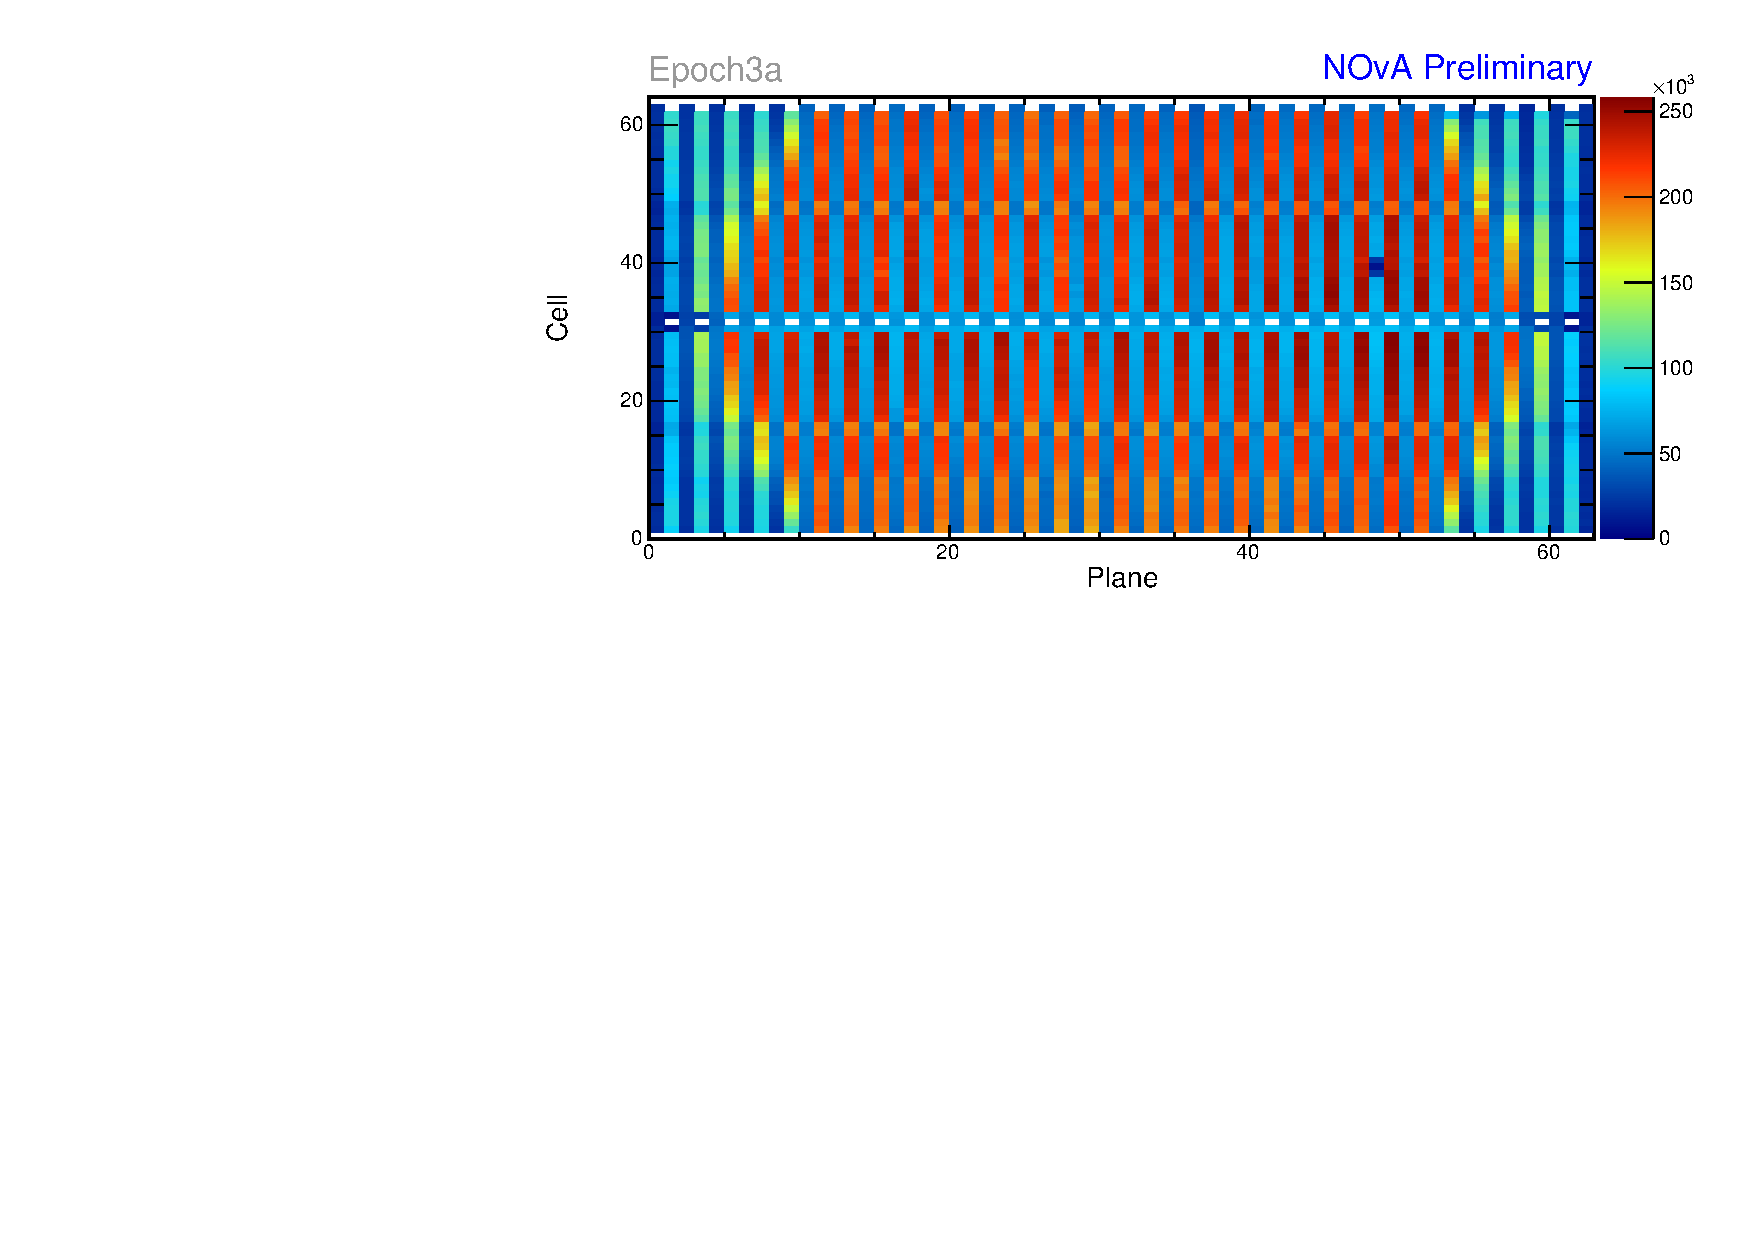
\includegraphics[width=\textwidth]{Plots/Attenprofs_P3Data_CellPlane_Epoch3a.pdf}
\end{subfigure}
\begin{subfigure}[b]{\textwidth}
\centering
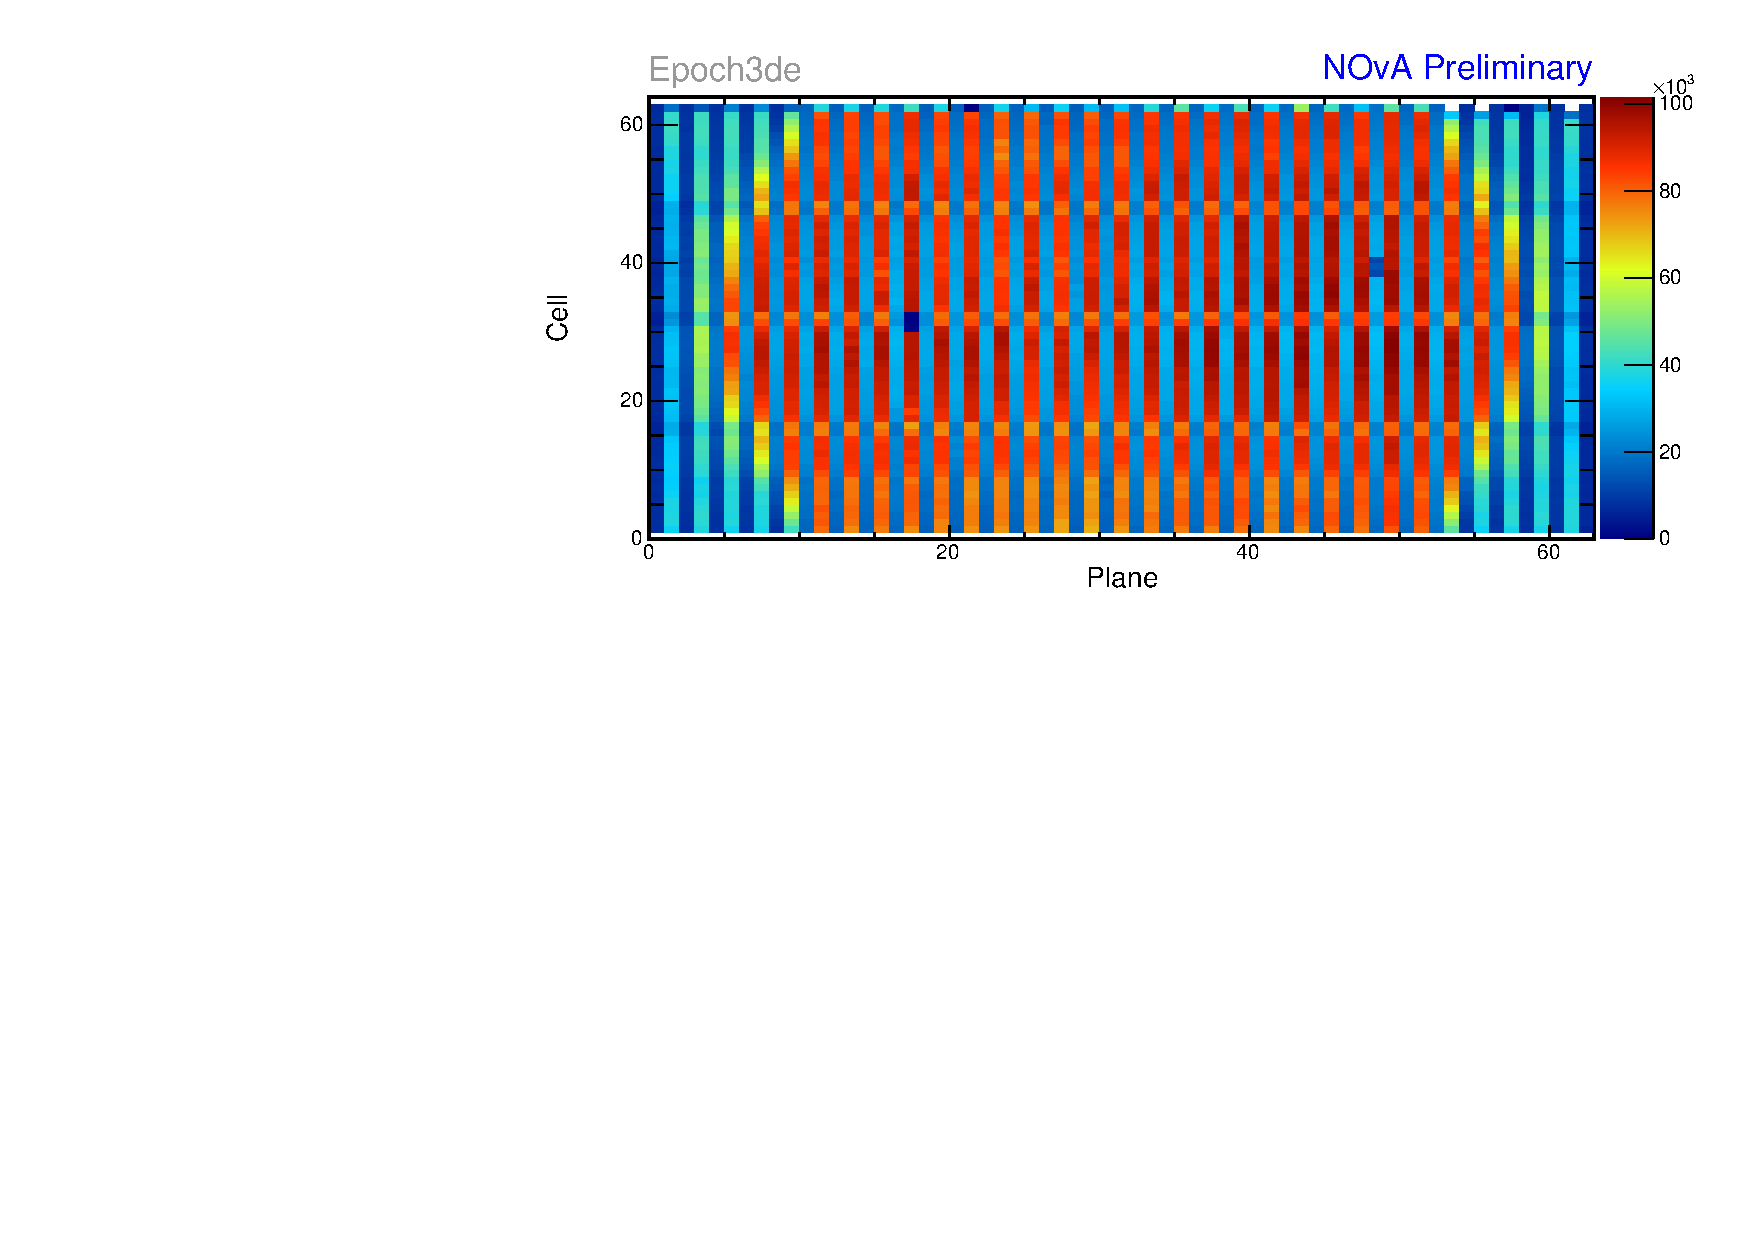
\includegraphics[width=\textwidth]{Plots/Attenprofs_P3Data_CellPlane_Epoch3de.pdf}
\end{subfigure}
\caption{Distribution of events in the period 3, epoch 3a Test Beam data calibration sample.}
\end{figure}

\begin{figure}[!hbtp]
\centering
\begin{subfigure}[b]{\textwidth}
\centering
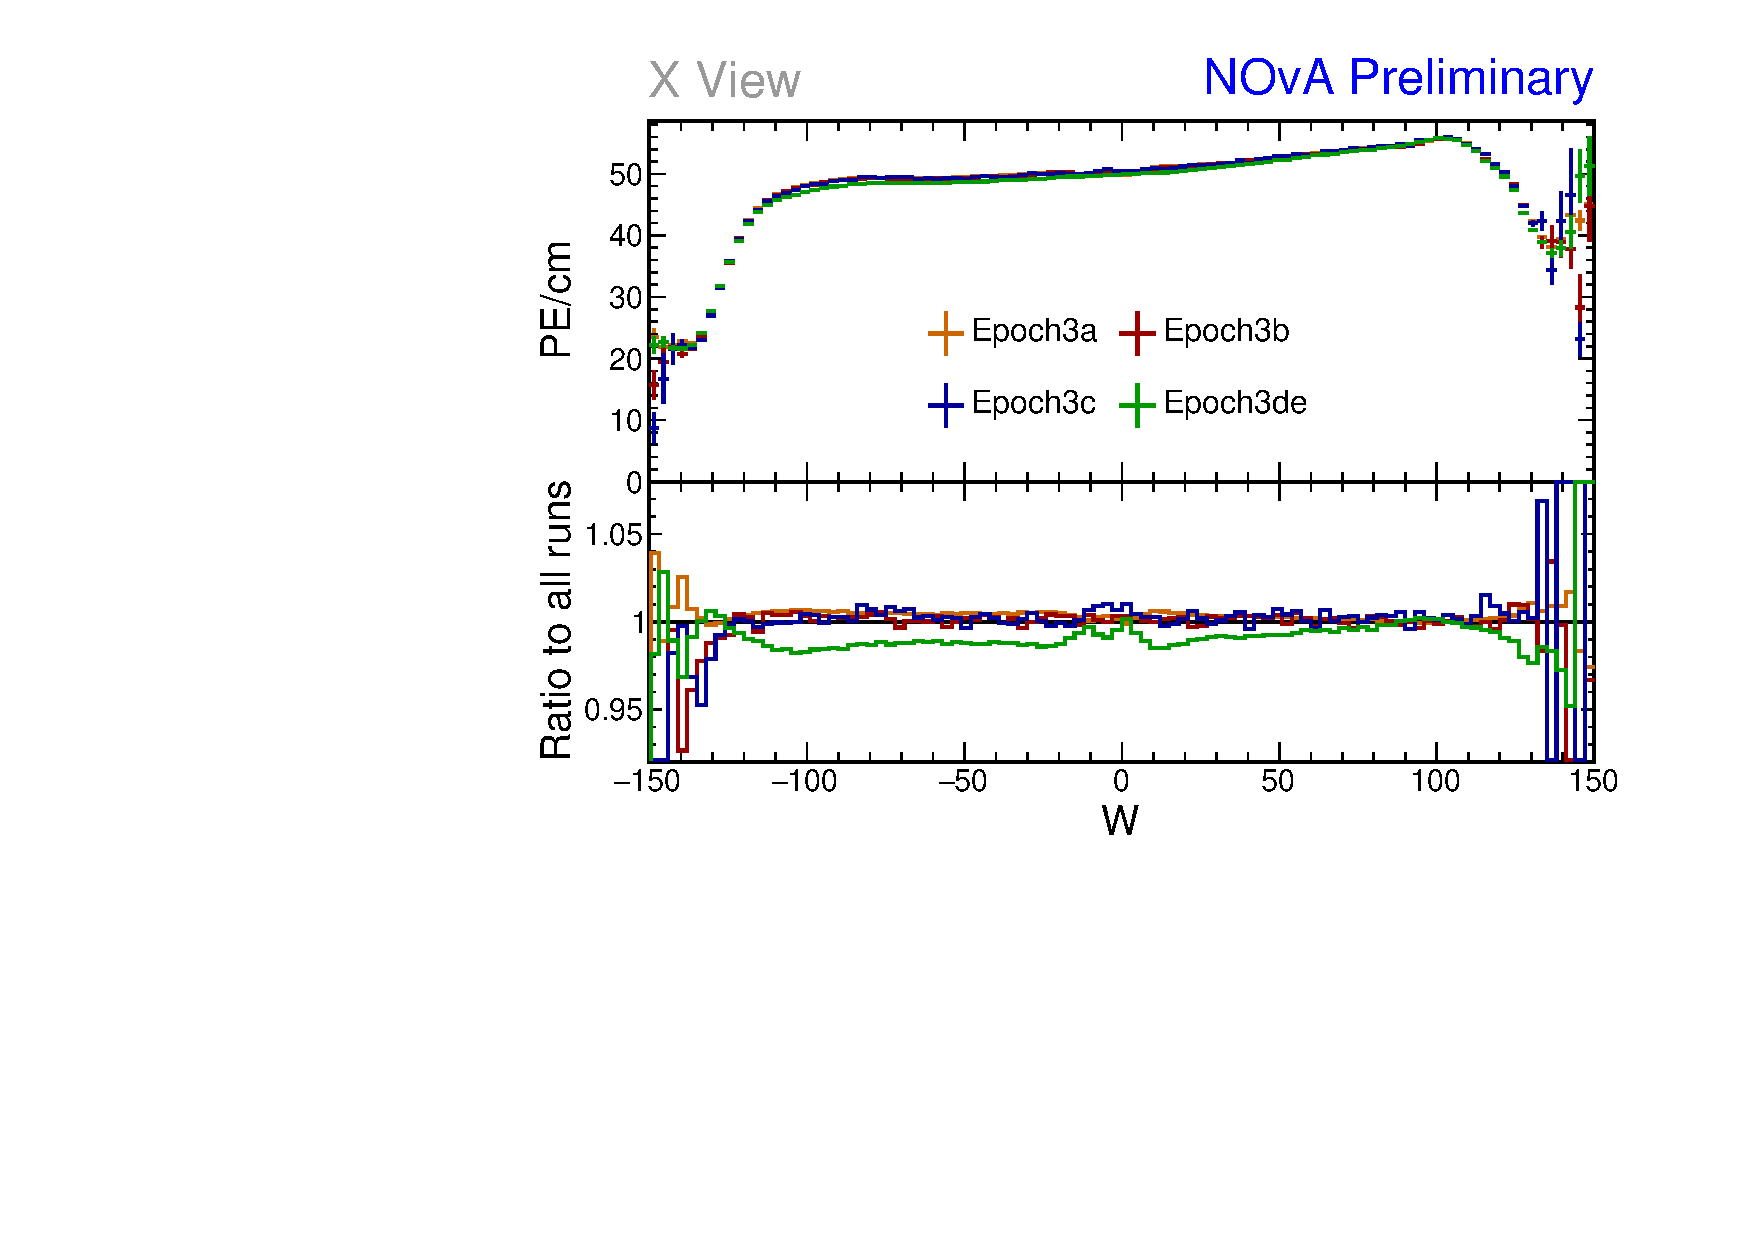
\includegraphics[width=\textwidth]{Plots/Attenprofs_P3Data_WPE_corr_xy_X_Combined.pdf}
\end{subfigure}
\begin{subfigure}[b]{\textwidth}
\centering
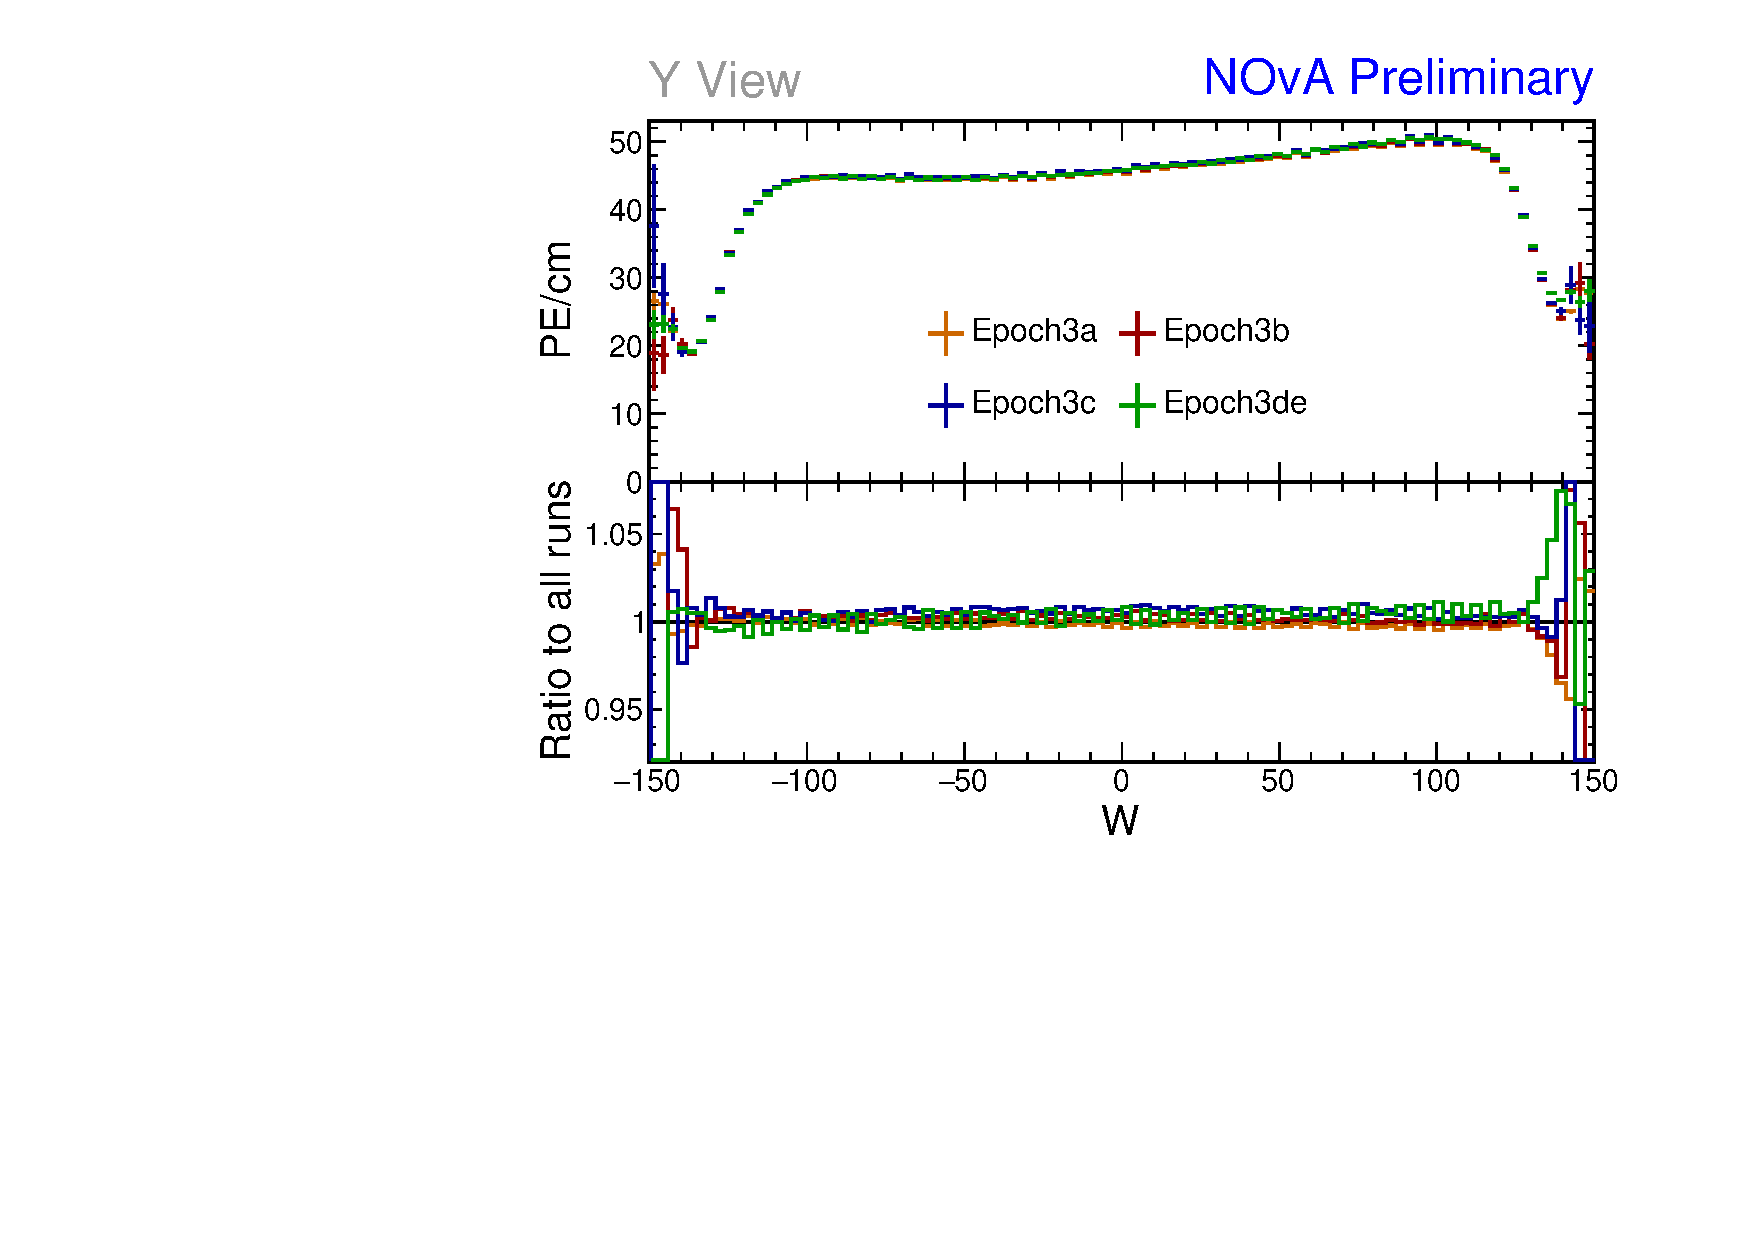
\includegraphics[width=\textwidth]{Plots/Attenprofs_P3Data_WPE_corr_xy_Y_Combined.pdf}
\end{subfigure}
\caption{Uncorrected average energy response as a function of the position within a cell (w) for epochs in period 3.}
\label{figCalibhistWPE_period3}
\end{figure}

\begin{figure}[!hbtp]
\centering
\begin{subfigure}[b]{\textwidth}
\centering
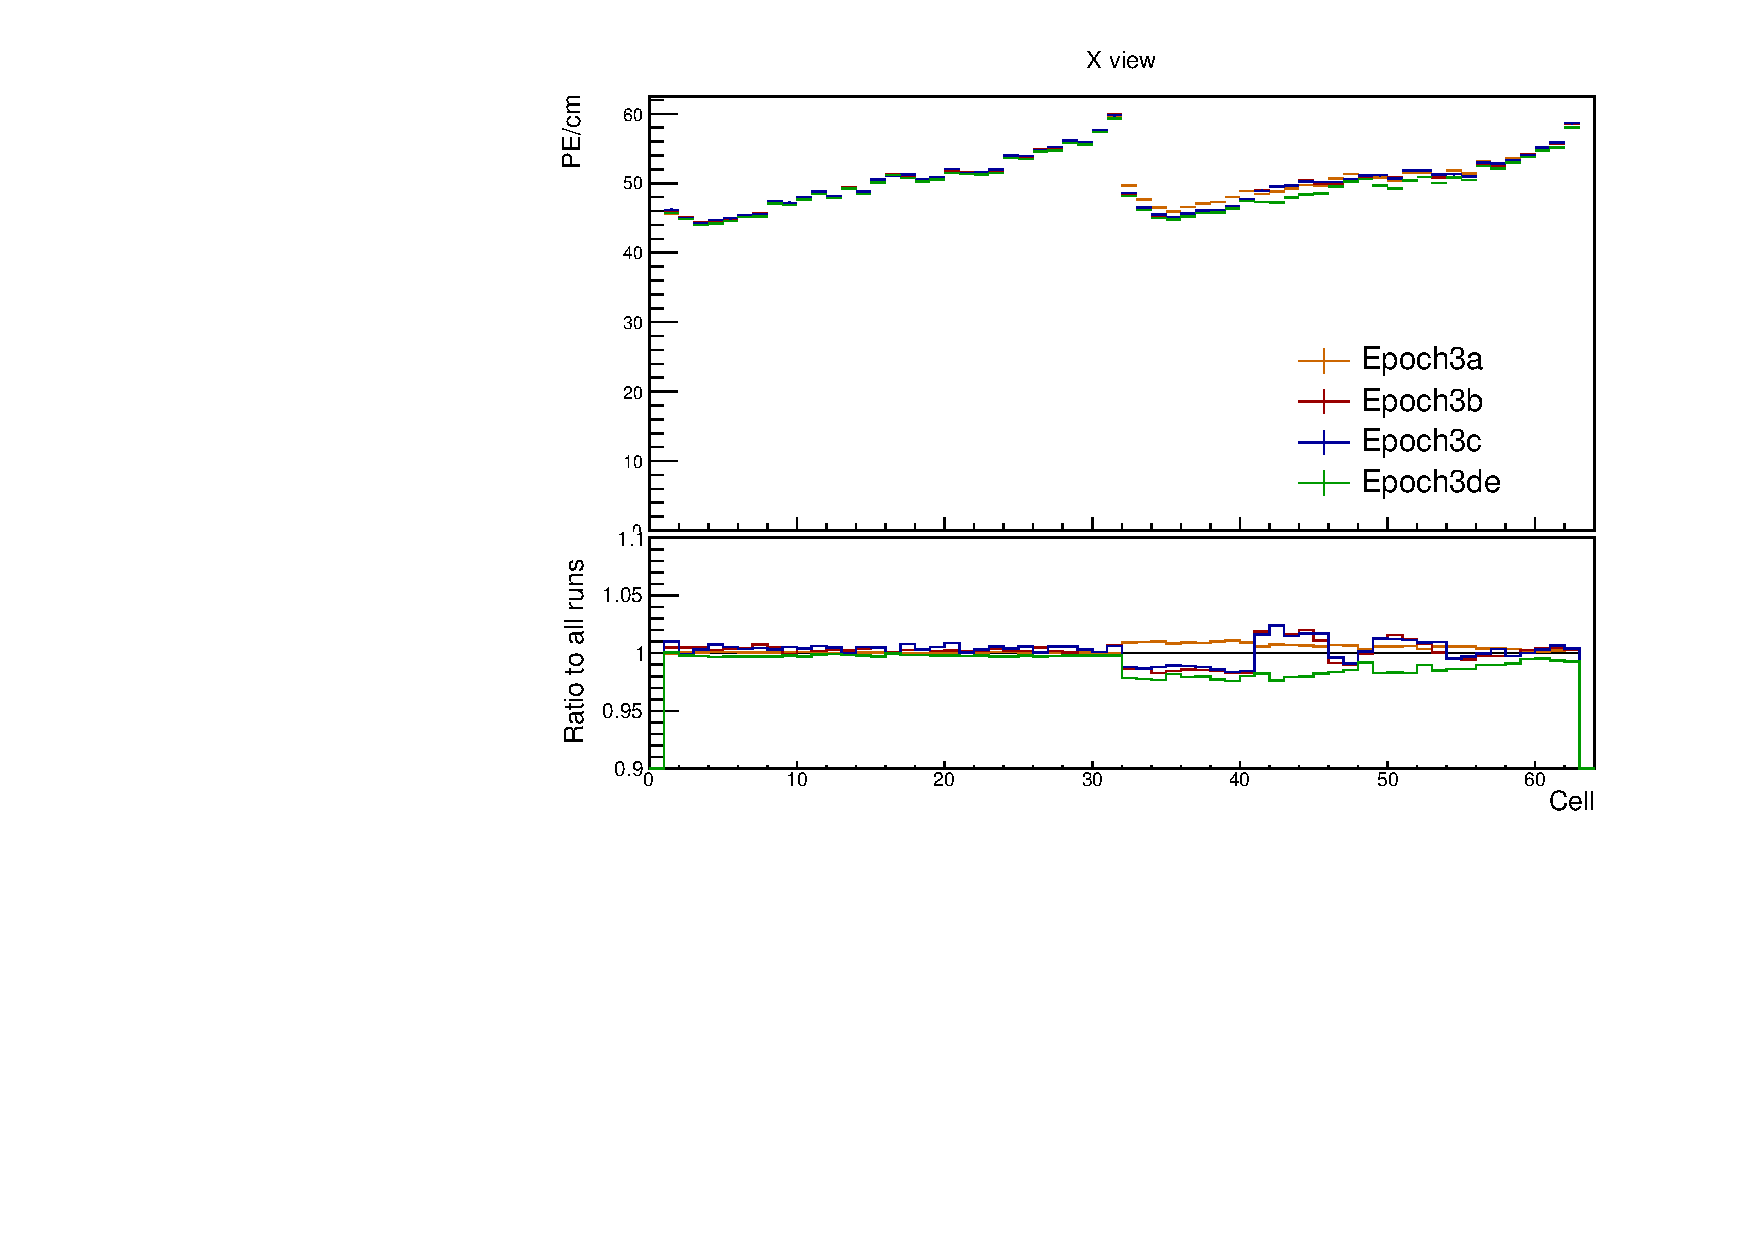
\includegraphics[width=\textwidth]{Plots/Attenprofs_P3Data_CellPE_X_Combined.pdf}
\end{subfigure}
\begin{subfigure}[b]{\textwidth}
\centering
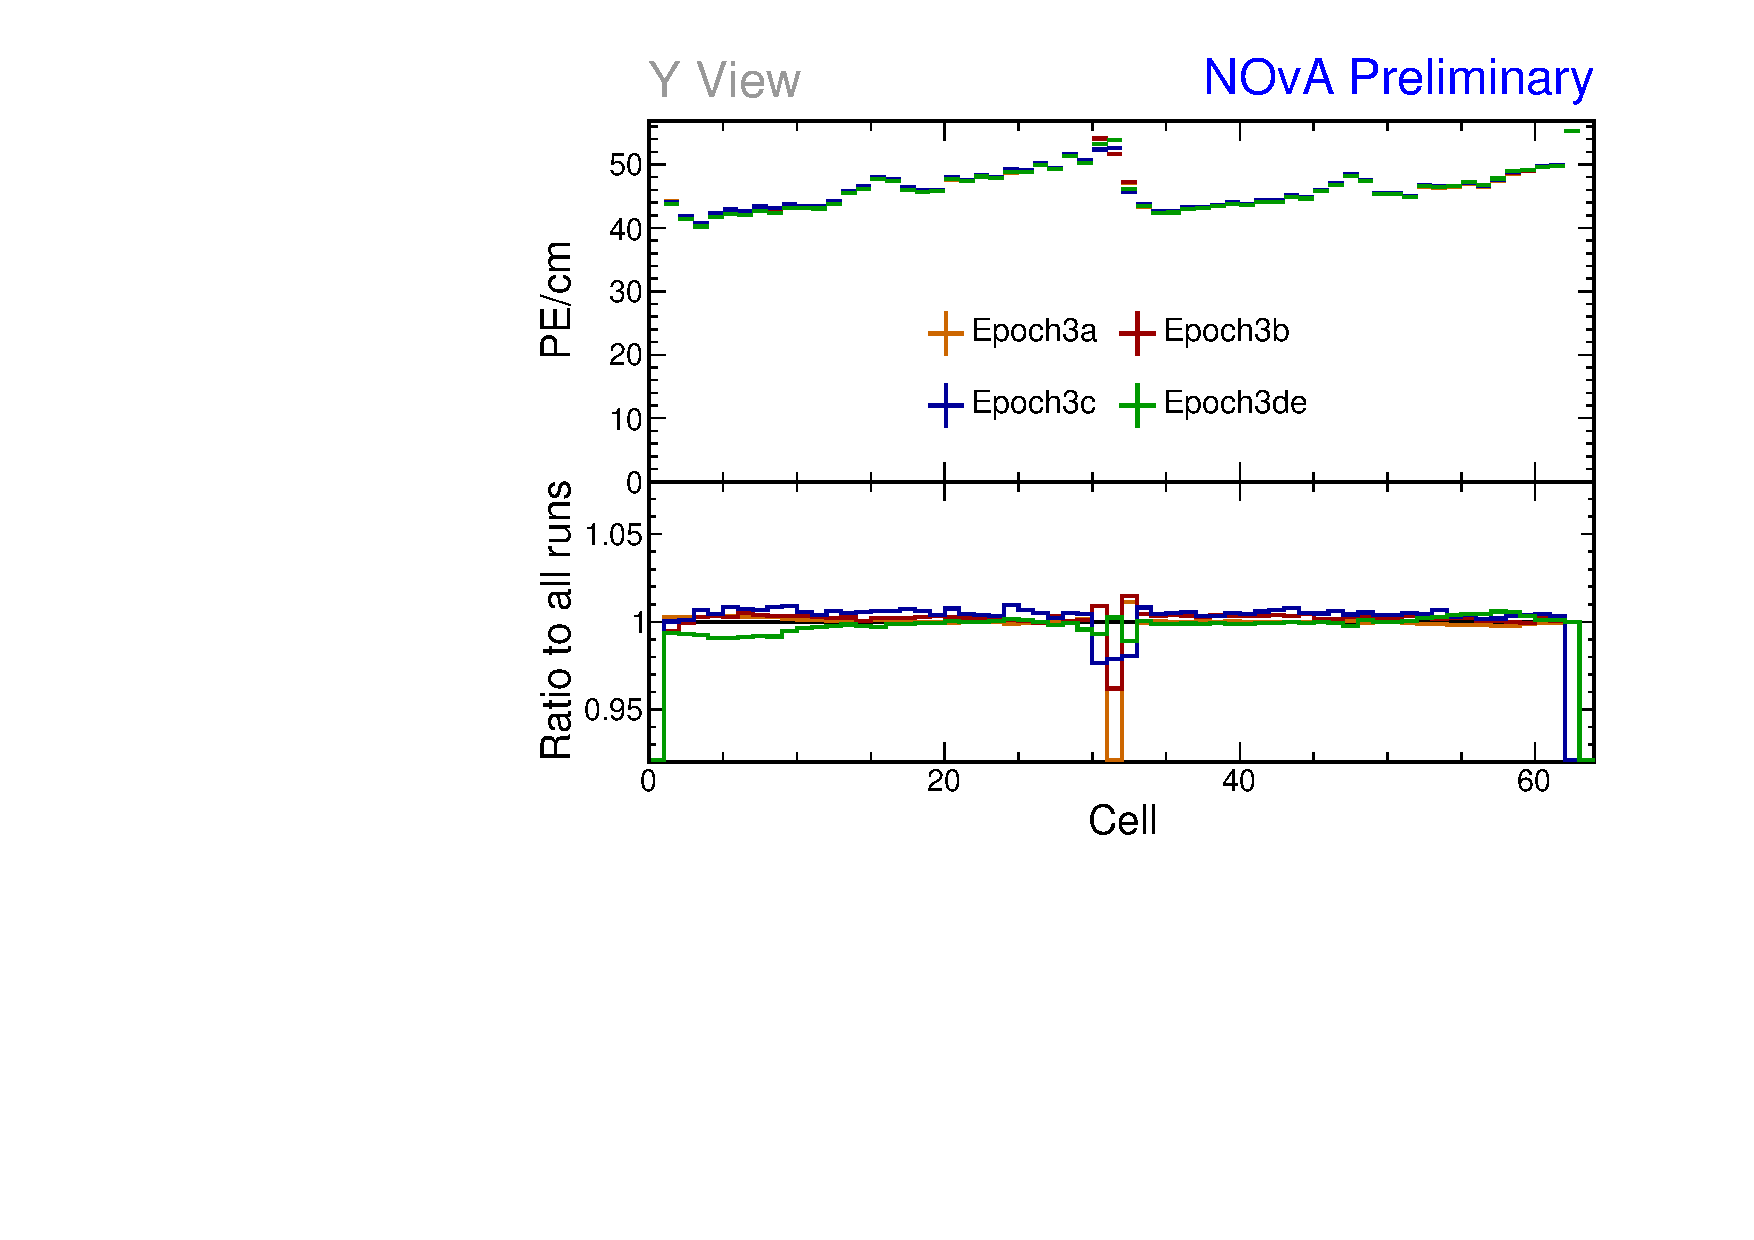
\includegraphics[width=\textwidth]{Plots/Attenprofs_P3Data_CellPE_Y_Combined.pdf}
\end{subfigure}
\caption{Uncorrected average energy response as a function of cells for epochs in period 3.}
\label{figCalibhistCellPE_period3}
\end{figure}

\begin{figure}[!hbtp]
\centering
\begin{subfigure}[b]{\textwidth}
\centering
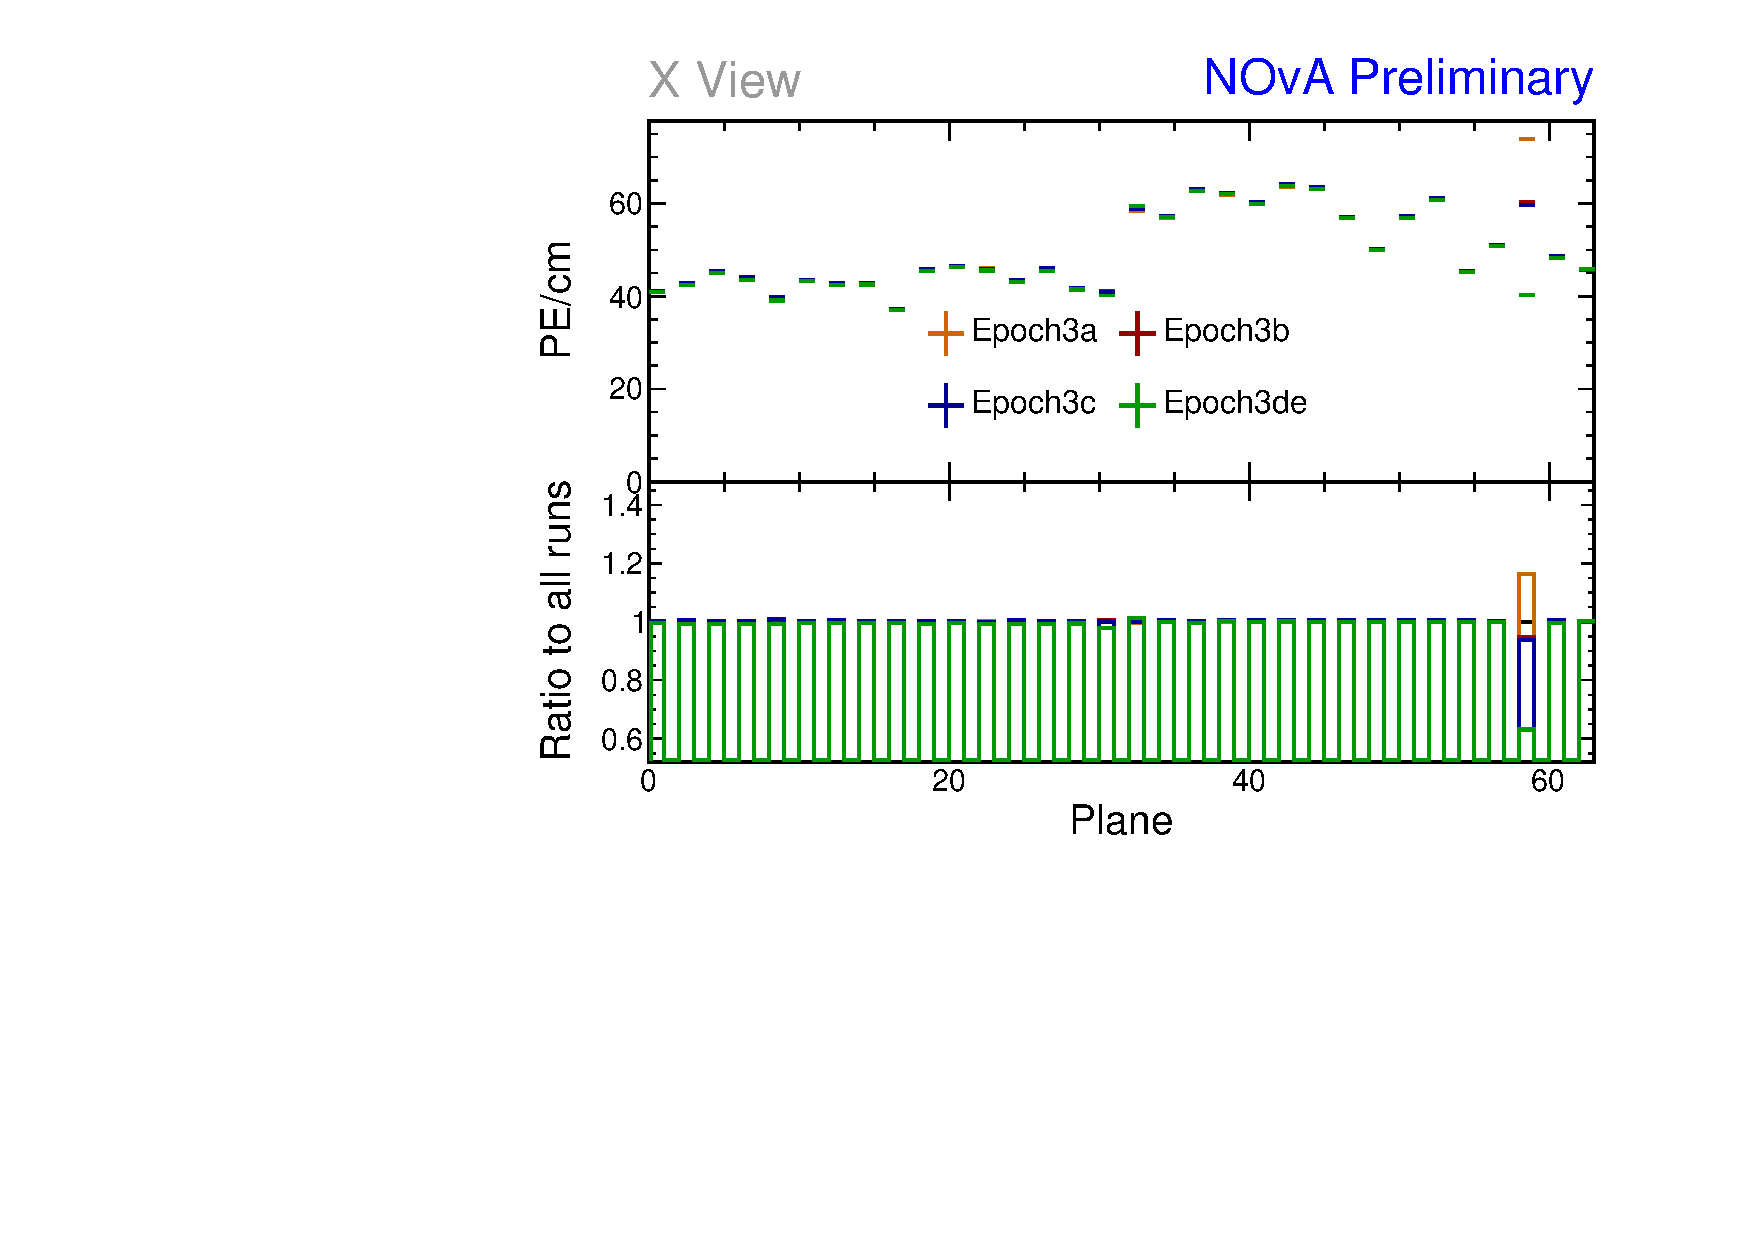
\includegraphics[width=\textwidth]{Plots/Attenprofs_P3Data_PlanePE_X_Combined.pdf}
\end{subfigure}
\begin{subfigure}[b]{\textwidth}
\centering
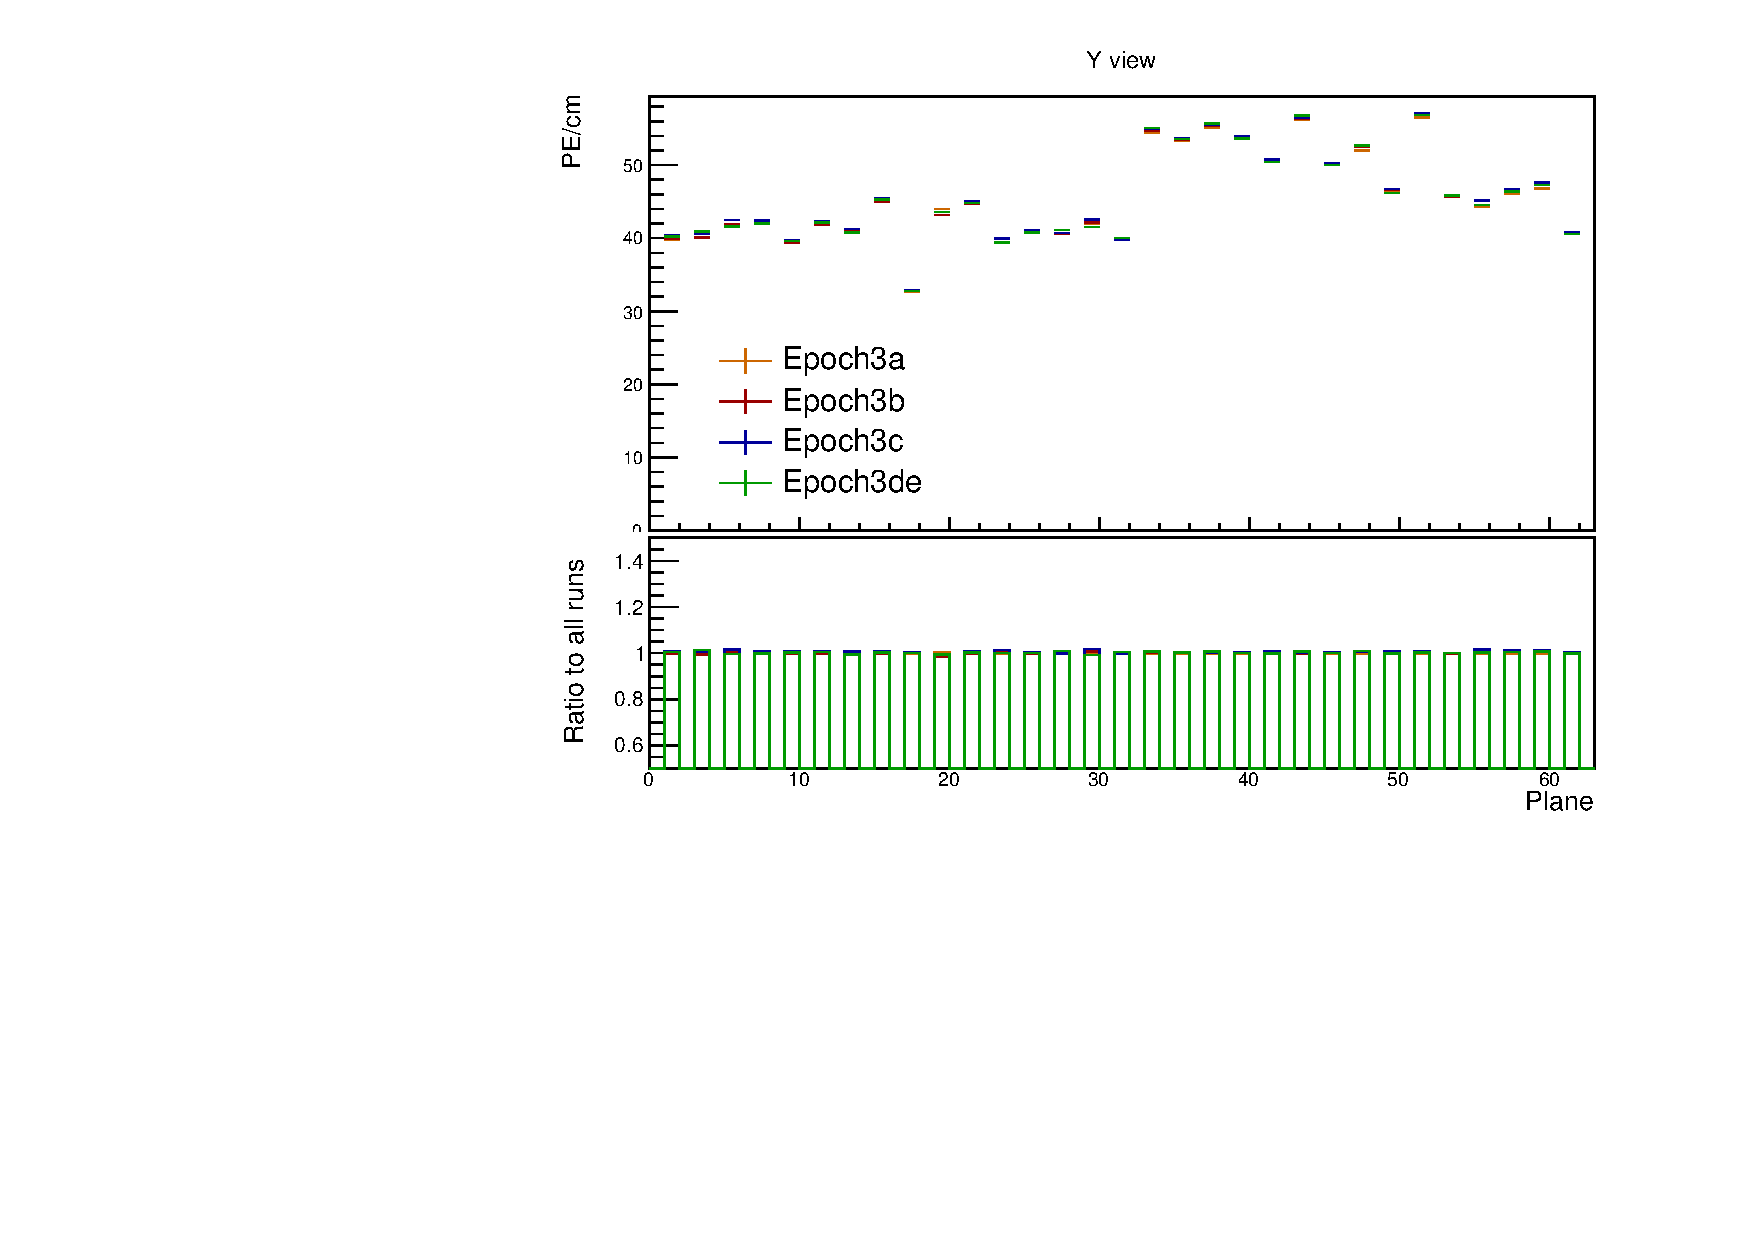
\includegraphics[width=\textwidth]{Plots/Attenprofs_P3Data_PlanePE_Y_Combined.pdf}
\end{subfigure}
\caption{Uncorrected average energy response as a function of planes for epochs in period 3.}
\label{figCalibhistPlanePE_period3}
\end{figure}

\subsubsection{Relative calibration results}

\subsubsection*{Combined epochs 3a, 3b and 3c}

\begin{figure}[!hbtp]
\centering
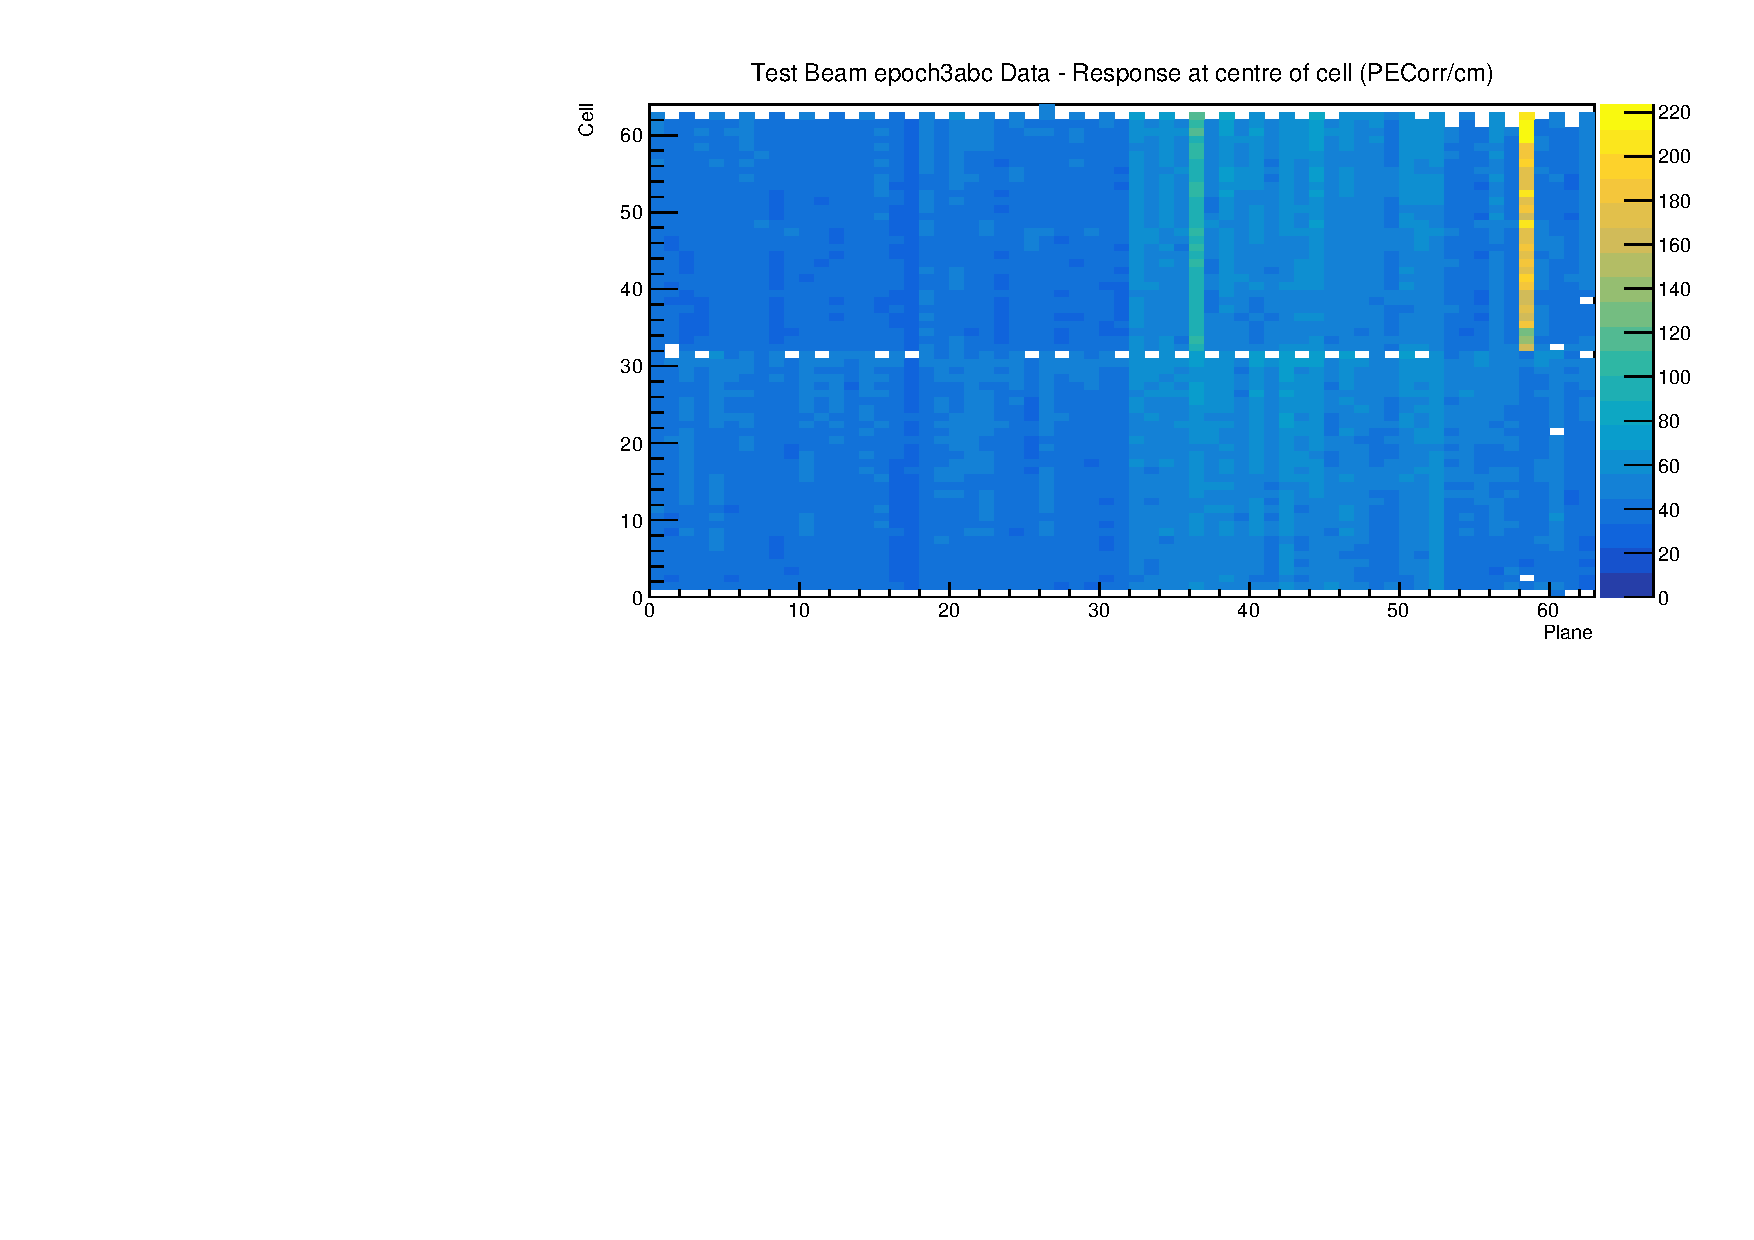
\includegraphics[width=\textwidth]{Plots/CellResponseAtCentre_epoch3abc.pdf}
\caption{Overview of the relative calibration results for the Teast Beam detector period 3, combined epochs 3a, 3b and 3c data. Each cell is represents the average corrected energy response (in PECorr/cm) in the centre of each cell. The blank cells are uncalibrated.}
\end{figure}

\subsubsection*{Combined epochs 3d and 3e}

\begin{figure}[!hbtp]
\centering
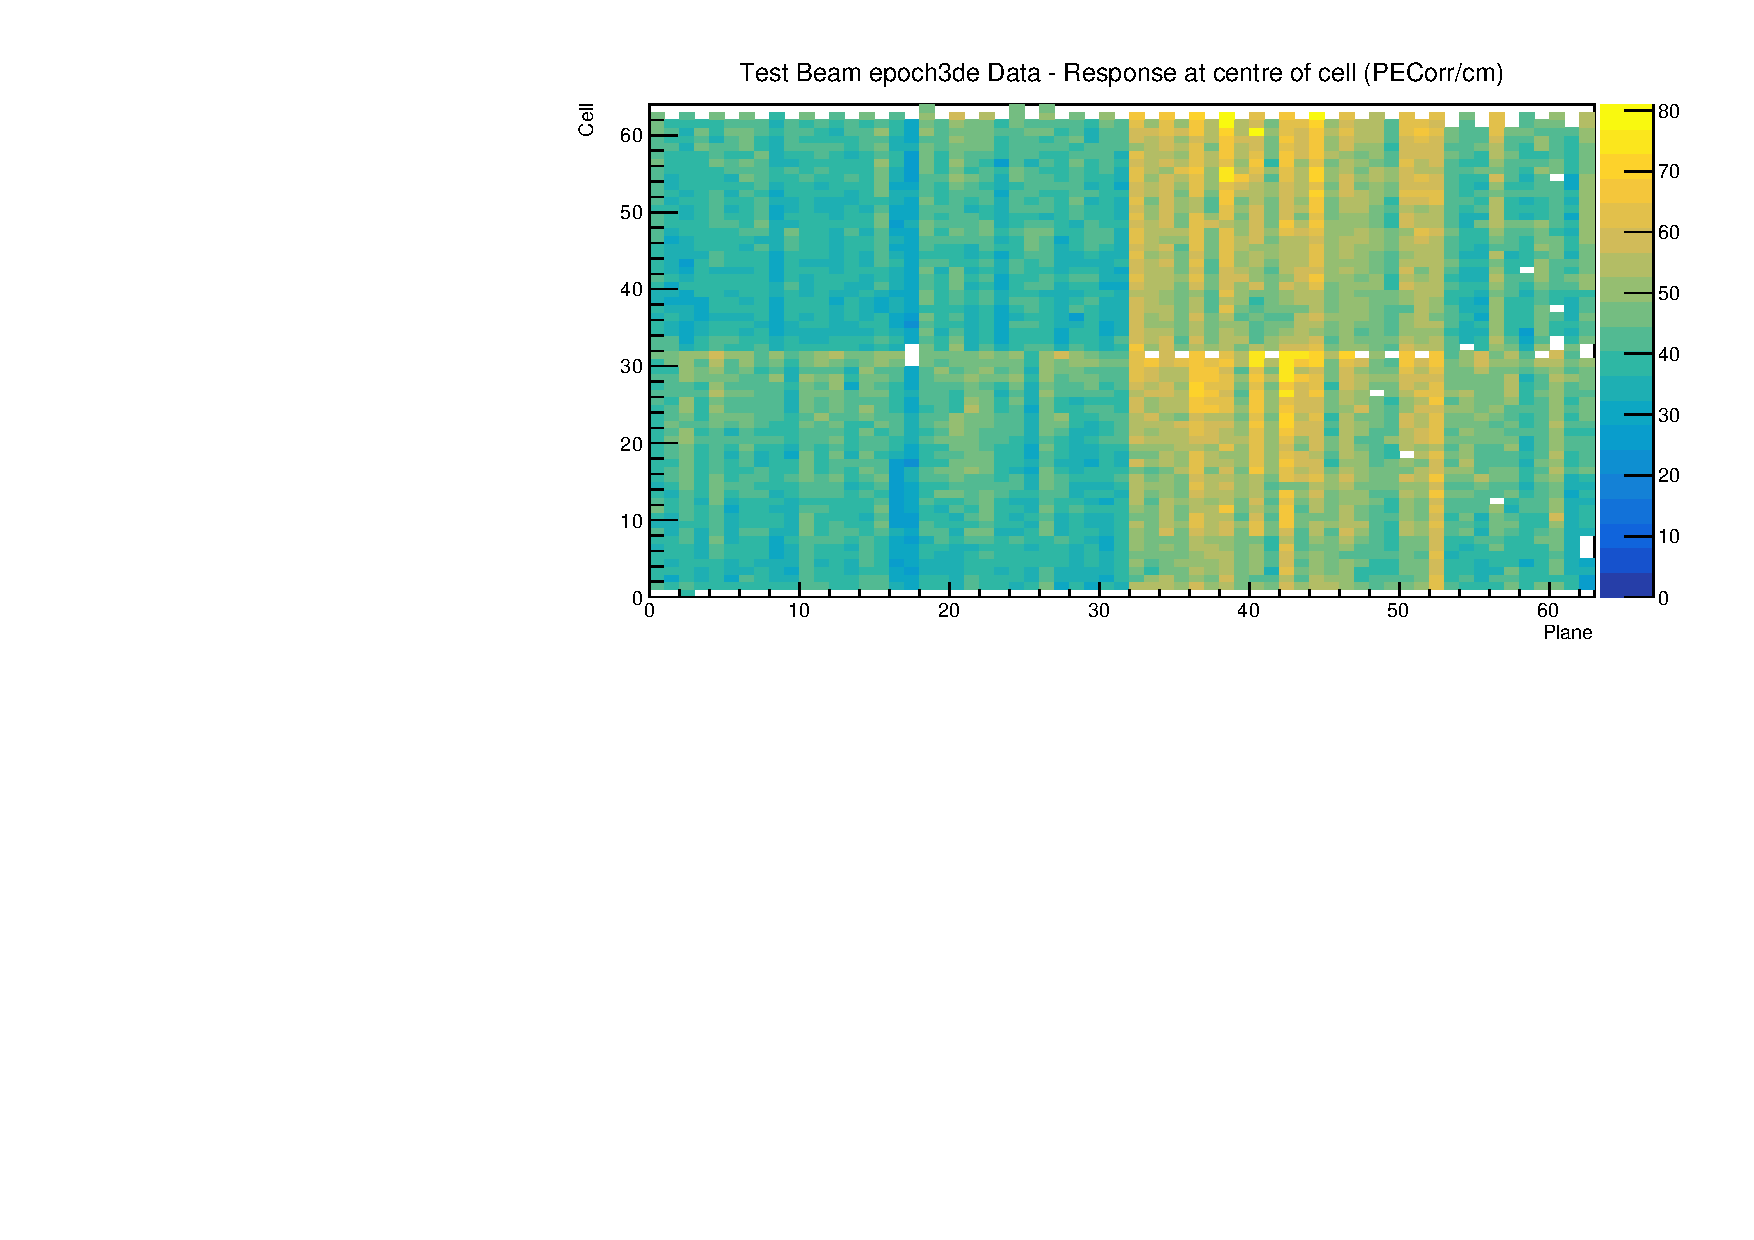
\includegraphics[width=\textwidth]{Plots/CellResponseAtCentre_epoch3de.pdf}
\caption{Overview of the relative calibration results for the Teast Beam detector period 3, combined epochs 3d and 3e data. Each cell is represents the average corrected energy response (in PECorr/cm) in the centre of each cell. The blank cells are uncalibrated.}
\end{figure}

\subsection{Period 4}

\begin{figure}[!hbtp]
\centering
\begin{subfigure}[b]{\textwidth}
\centering
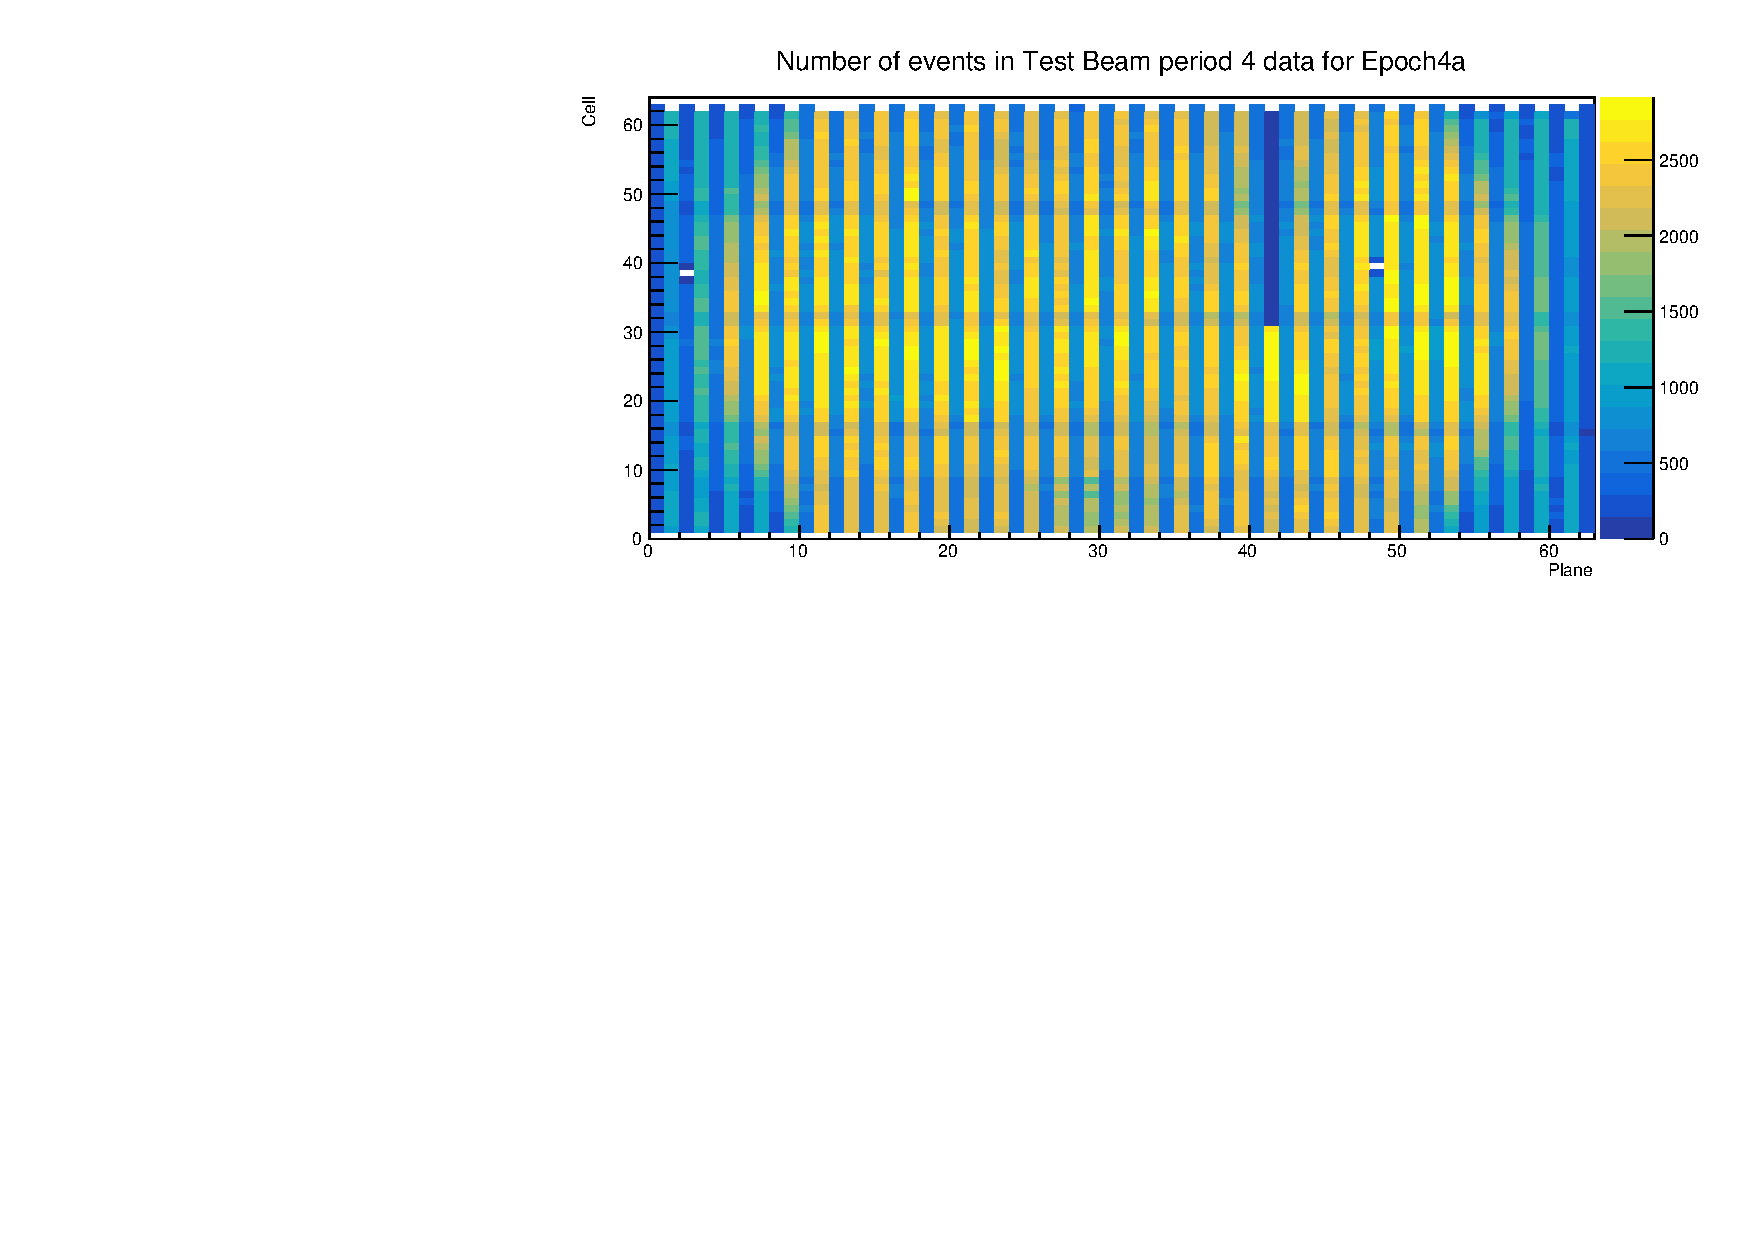
\includegraphics[width=.9\textwidth]{Plots/Attenprofs_P4Data_CellPlane_Epoch4a.pdf}
\end{subfigure}
\begin{subfigure}[b]{\textwidth}
\centering
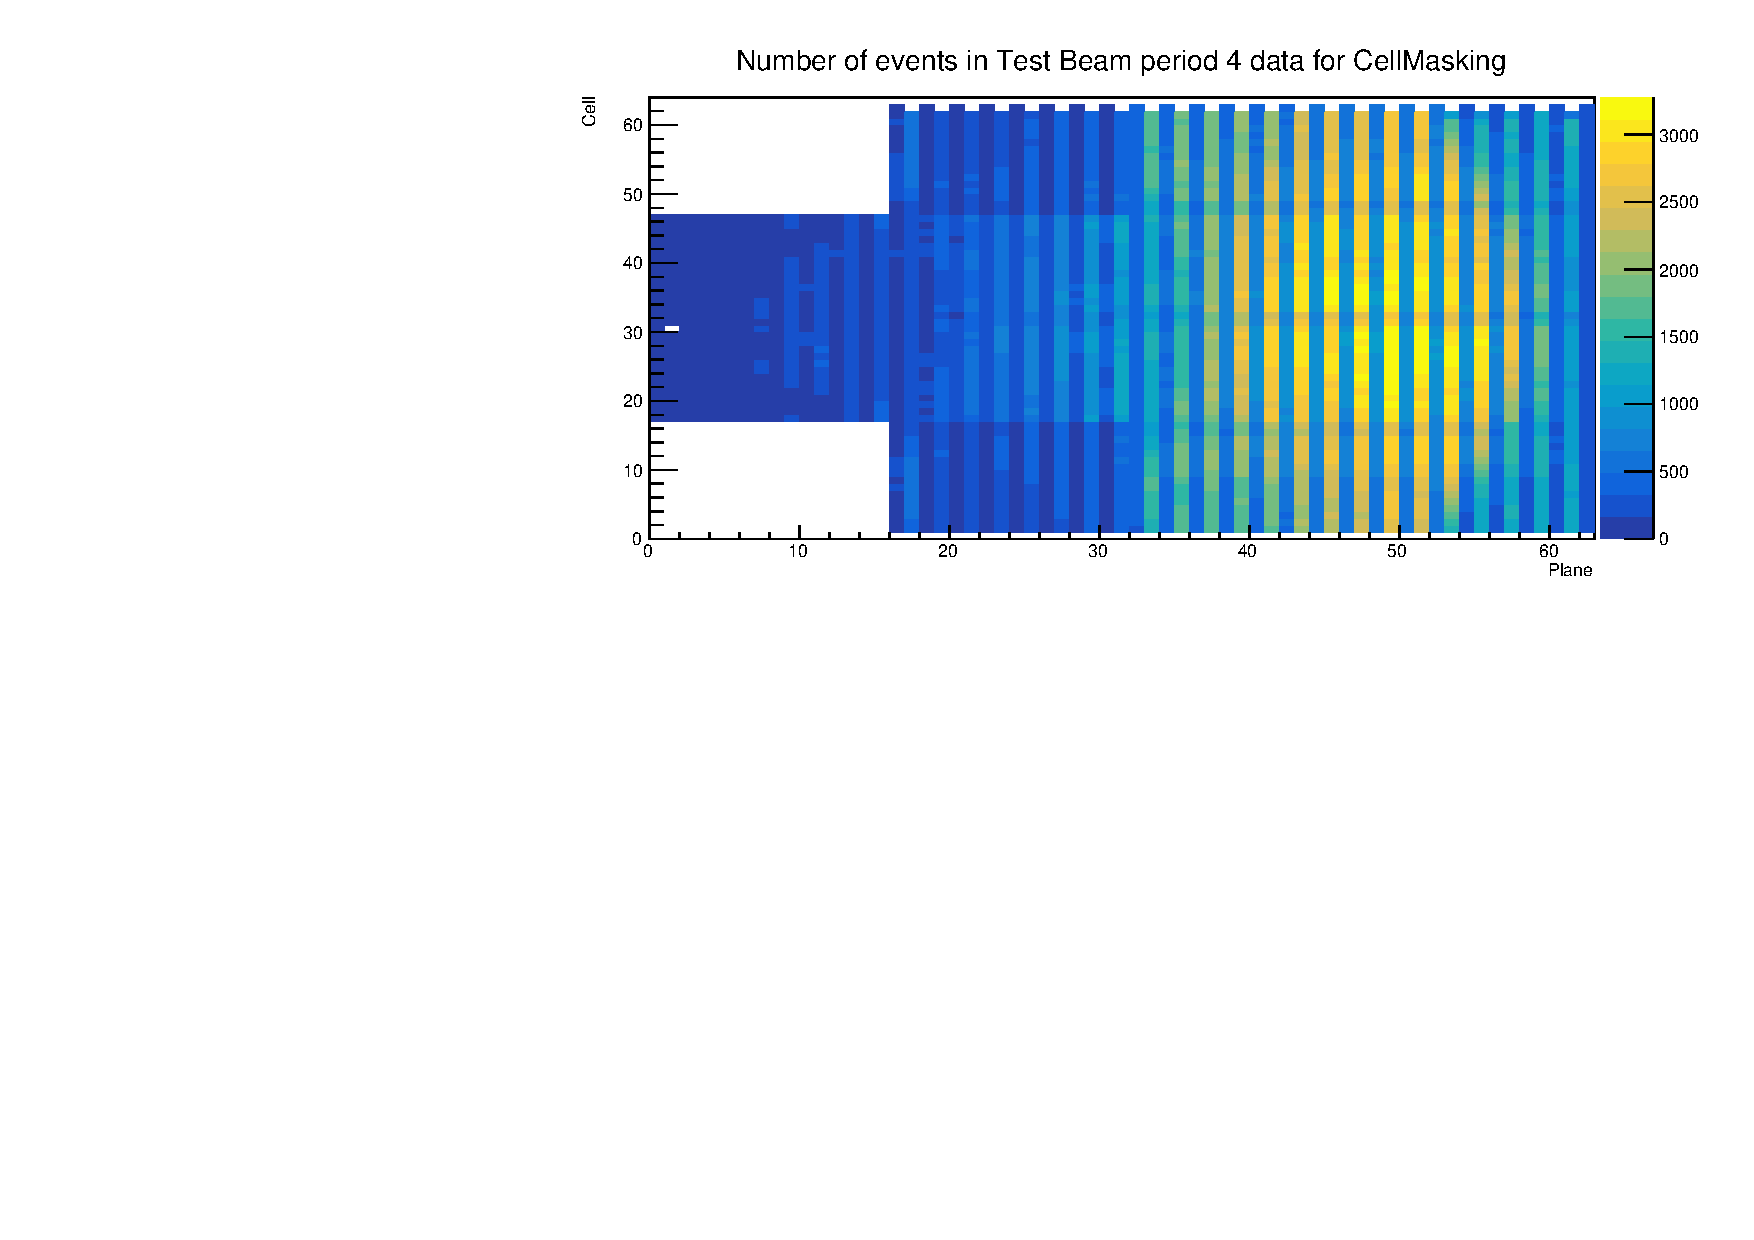
\includegraphics[width=.9\textwidth]{Plots/Attenprofs_P4Data_CellPlane_CellMasking.pdf}
\end{subfigure}
\begin{subfigure}[b]{\textwidth}
\centering
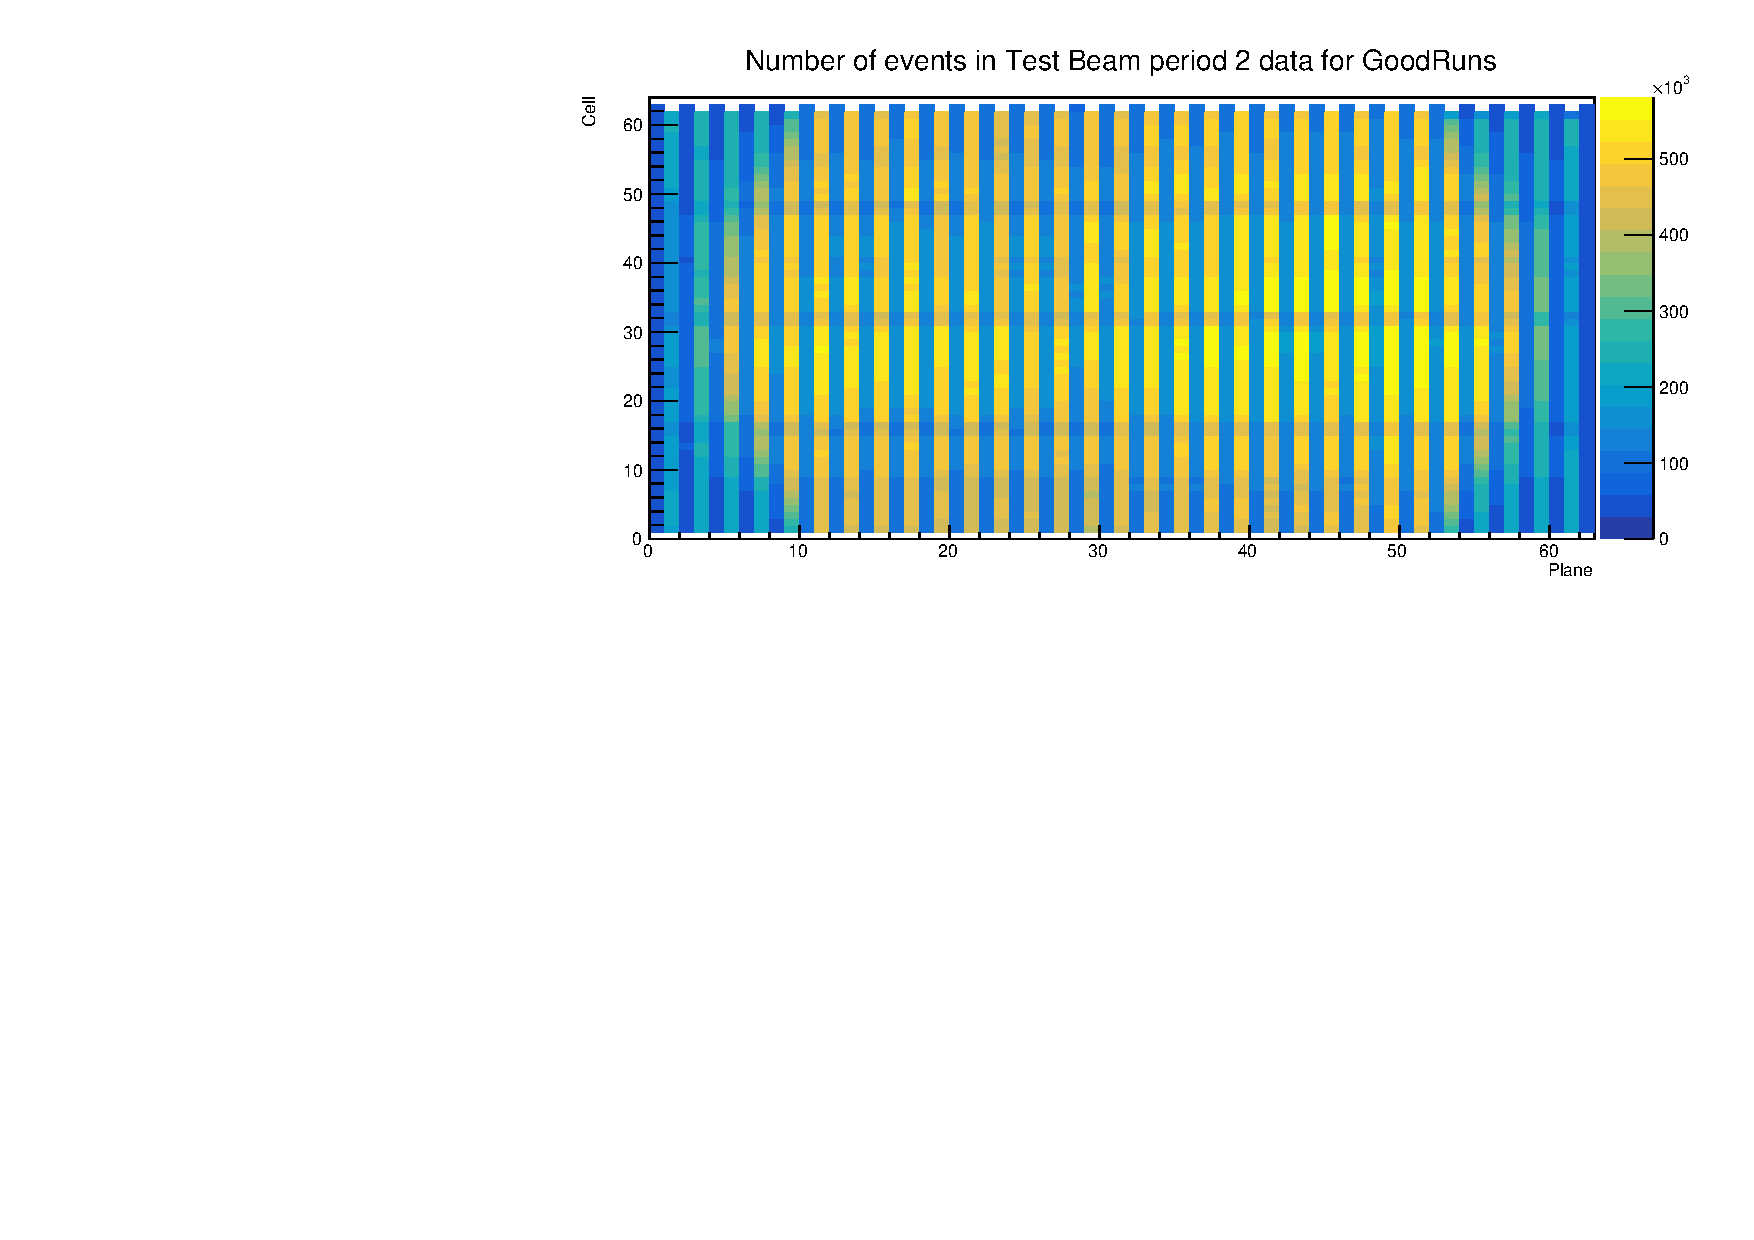
\includegraphics[width=.9\textwidth]{Plots/Attenprofs_P4Data_CellPlane_GoodRuns.pdf}
\end{subfigure}
\caption{Distribution of events in the Test Beam period 4 data calibration sample. The top plot shows the first three comissioning runs, the middle plot the status of the detector during the Cell Masking studies and the bottom plot shows the rest.}
\end{figure}

\begin{figure}[!hbtp]
\centering
\begin{subfigure}[b]{\textwidth}
\centering
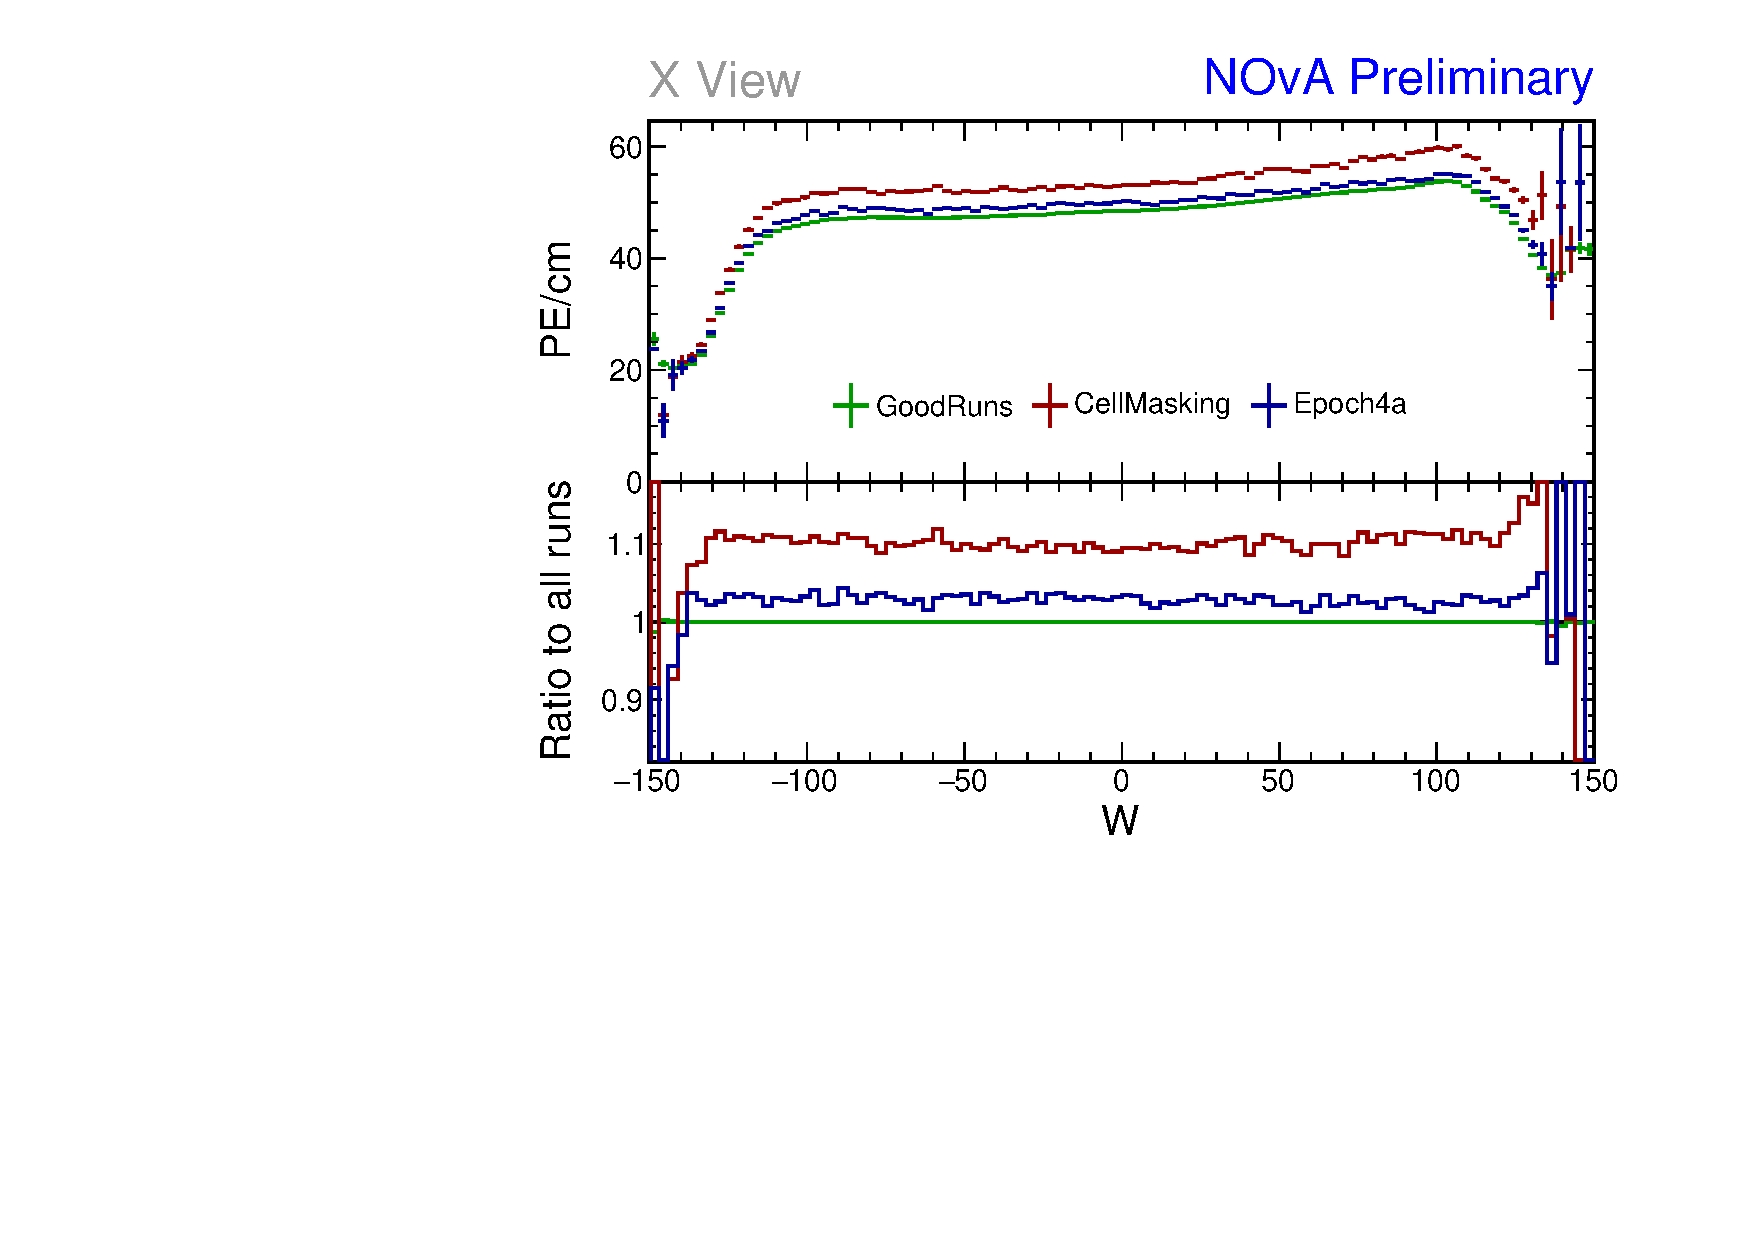
\includegraphics[width=\textwidth]{Plots/Attenprofs_P4Data_WPE_corr_xy_X_Combined.pdf}
\end{subfigure}
\begin{subfigure}[b]{\textwidth}
\centering
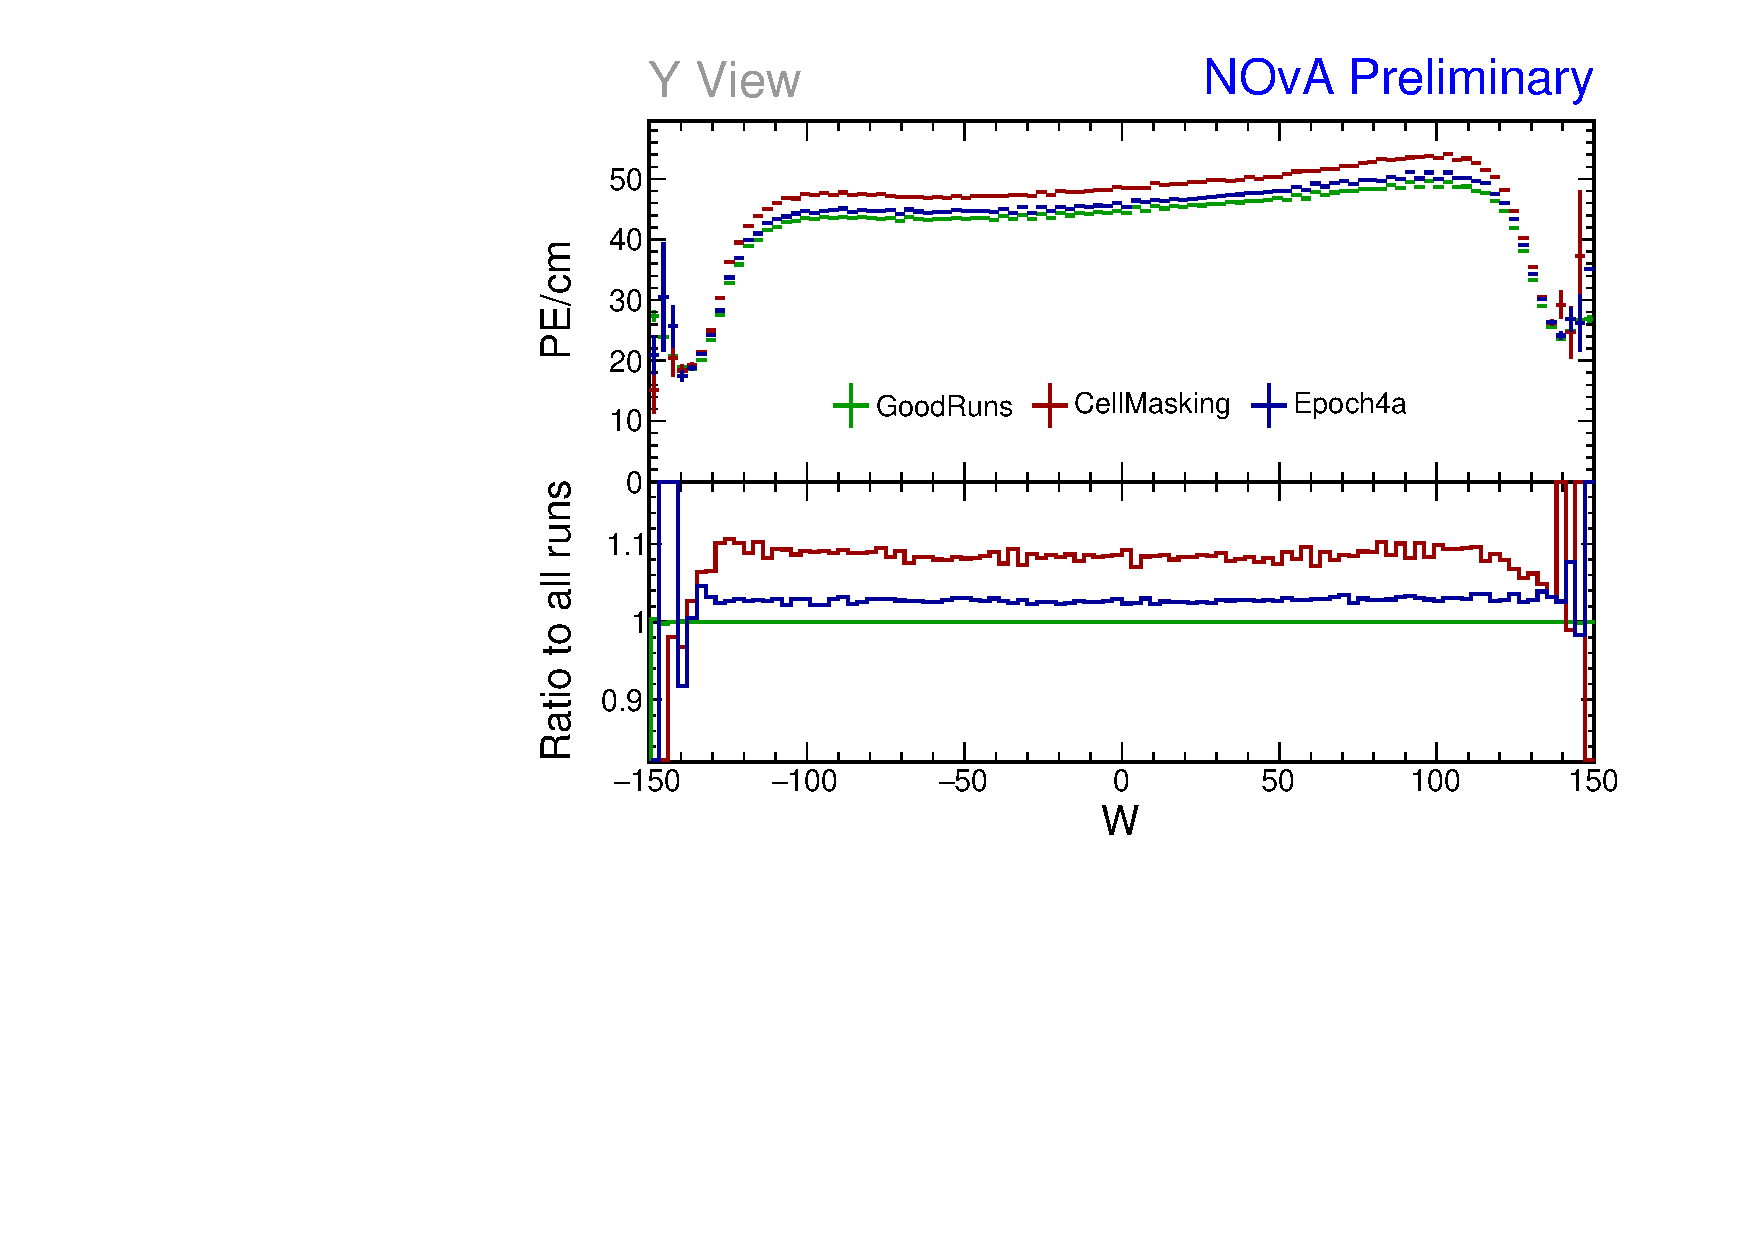
\includegraphics[width=\textwidth]{Plots/Attenprofs_P4Data_WPE_corr_xy_Y_Combined.pdf}
\end{subfigure}
\caption{Uncorrected average energy response as a function of the position within a cell (w) for epochs in period 4.}
\label{figCalibhistWPE_period4}
\end{figure}

\begin{figure}[!hbtp]
\centering
\begin{subfigure}[b]{\textwidth}
\centering
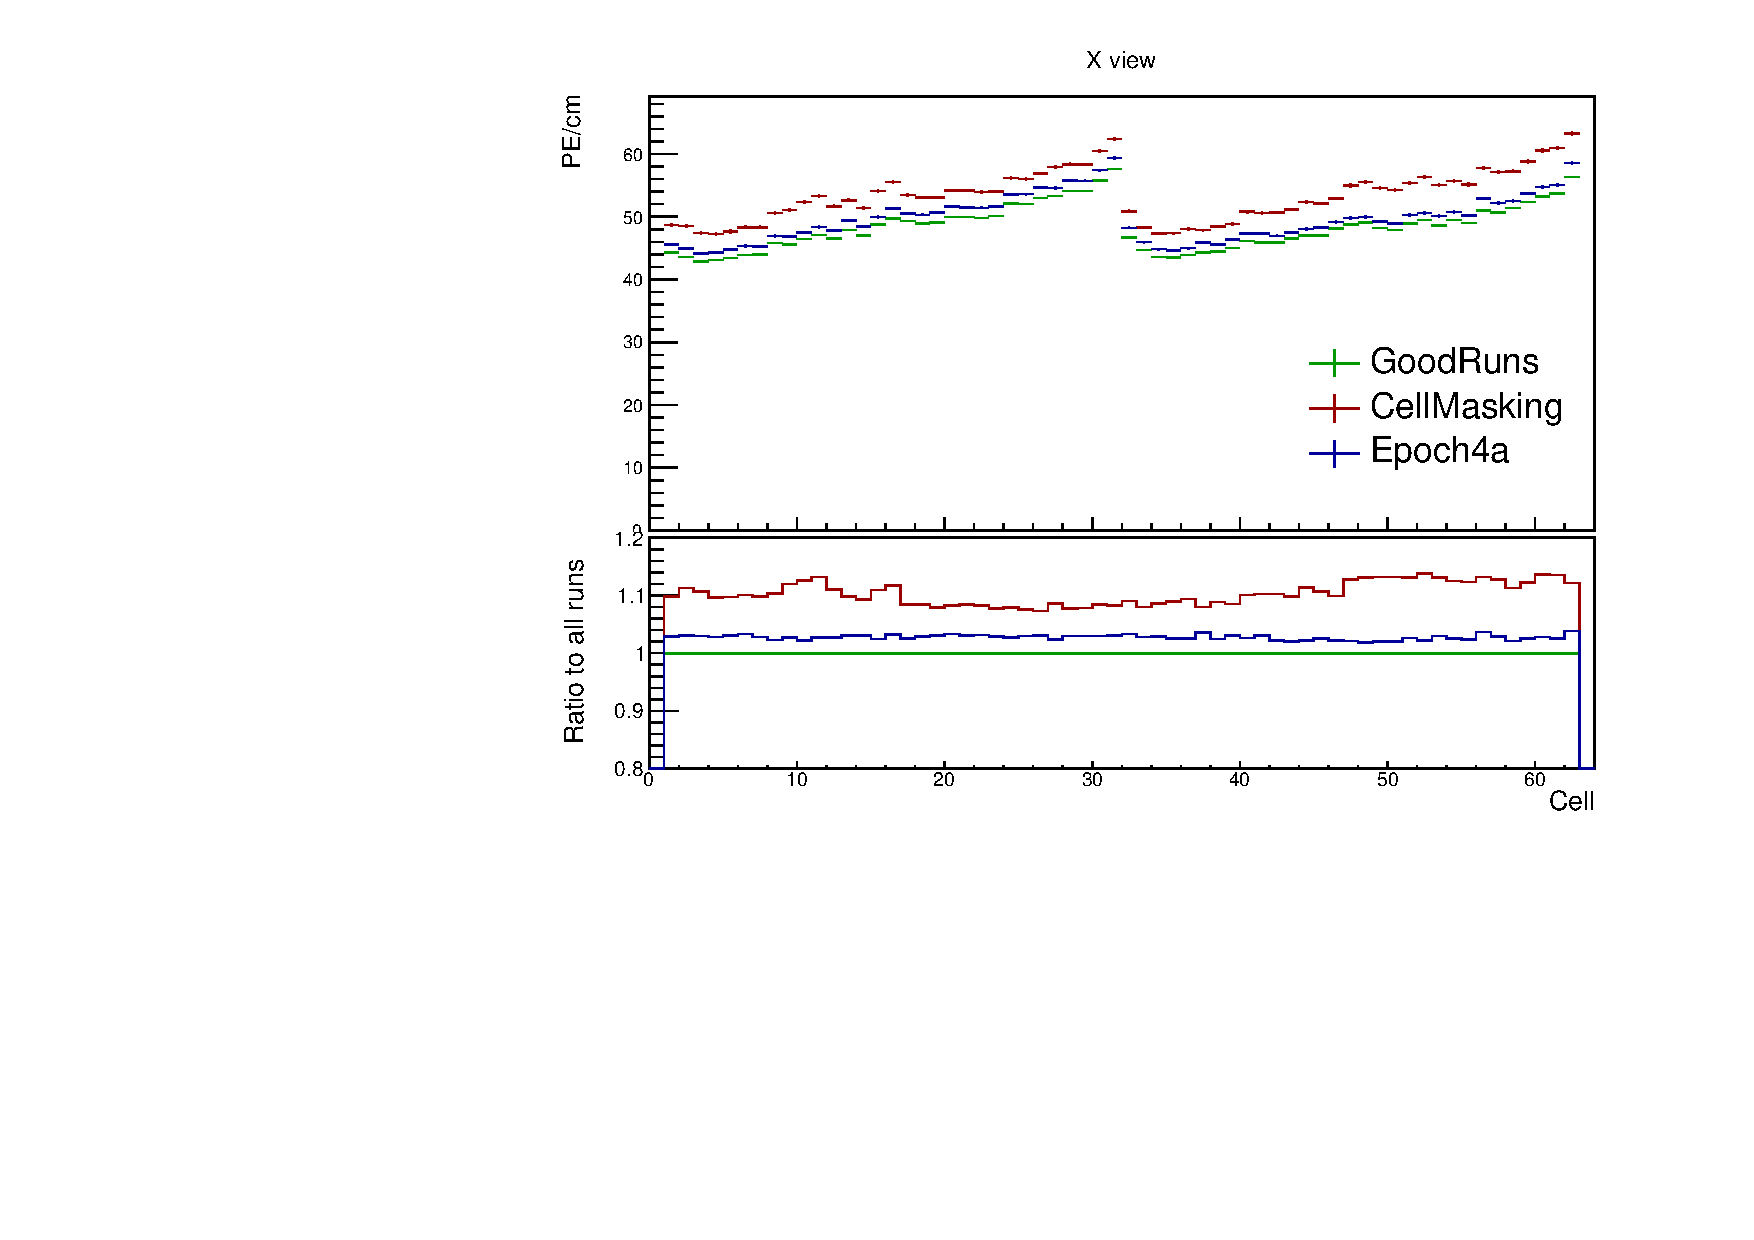
\includegraphics[width=\textwidth]{Plots/Attenprofs_P4Data_CellPE_X_Combined.pdf}
\end{subfigure}
\begin{subfigure}[b]{\textwidth}
\centering
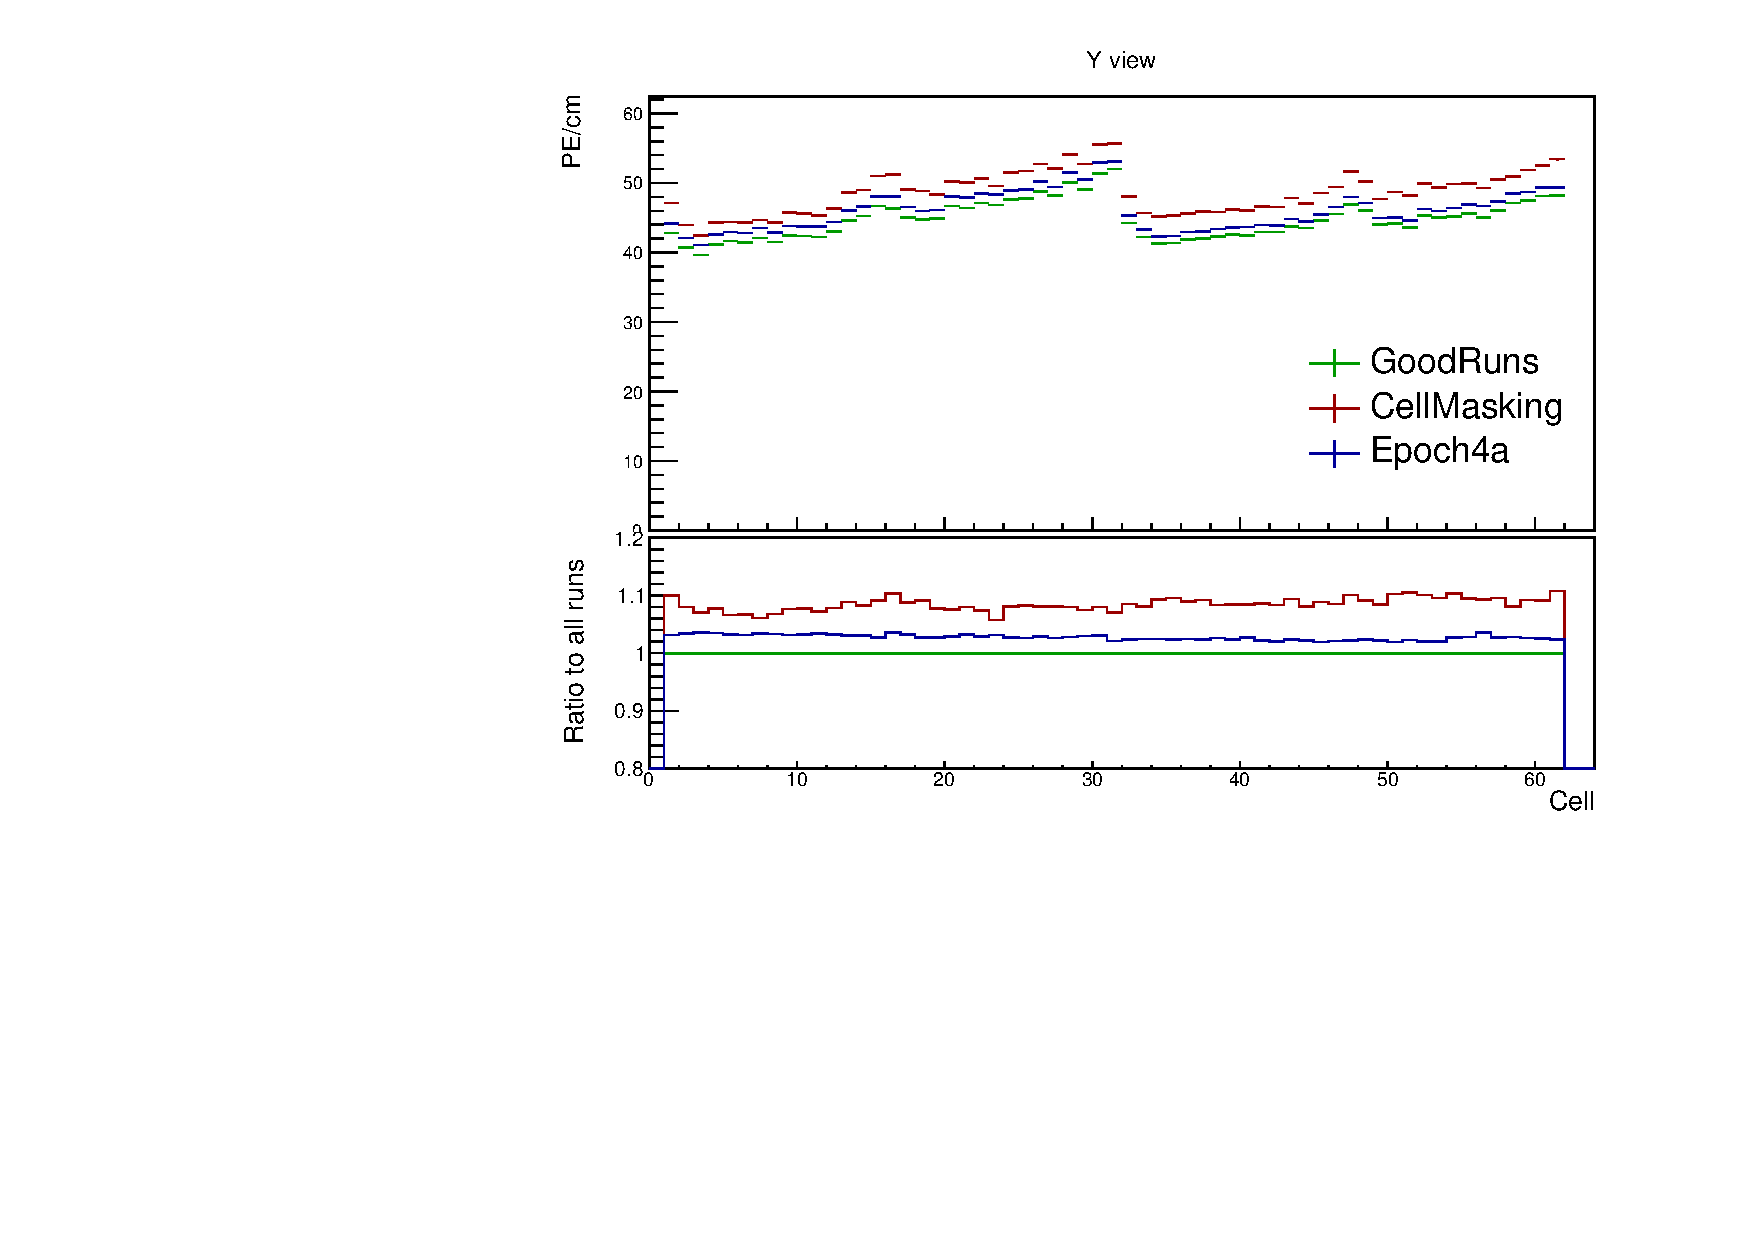
\includegraphics[width=\textwidth]{Plots/Attenprofs_P4Data_CellPE_Y_Combined.pdf}
\end{subfigure}
\caption{Uncorrected average energy response as a function of cells for epochs in period 4.}
\label{figCalibhistCellPE_period4}
\end{figure}

\begin{figure}[!hbtp]
\centering
\begin{subfigure}[b]{\textwidth}
\centering
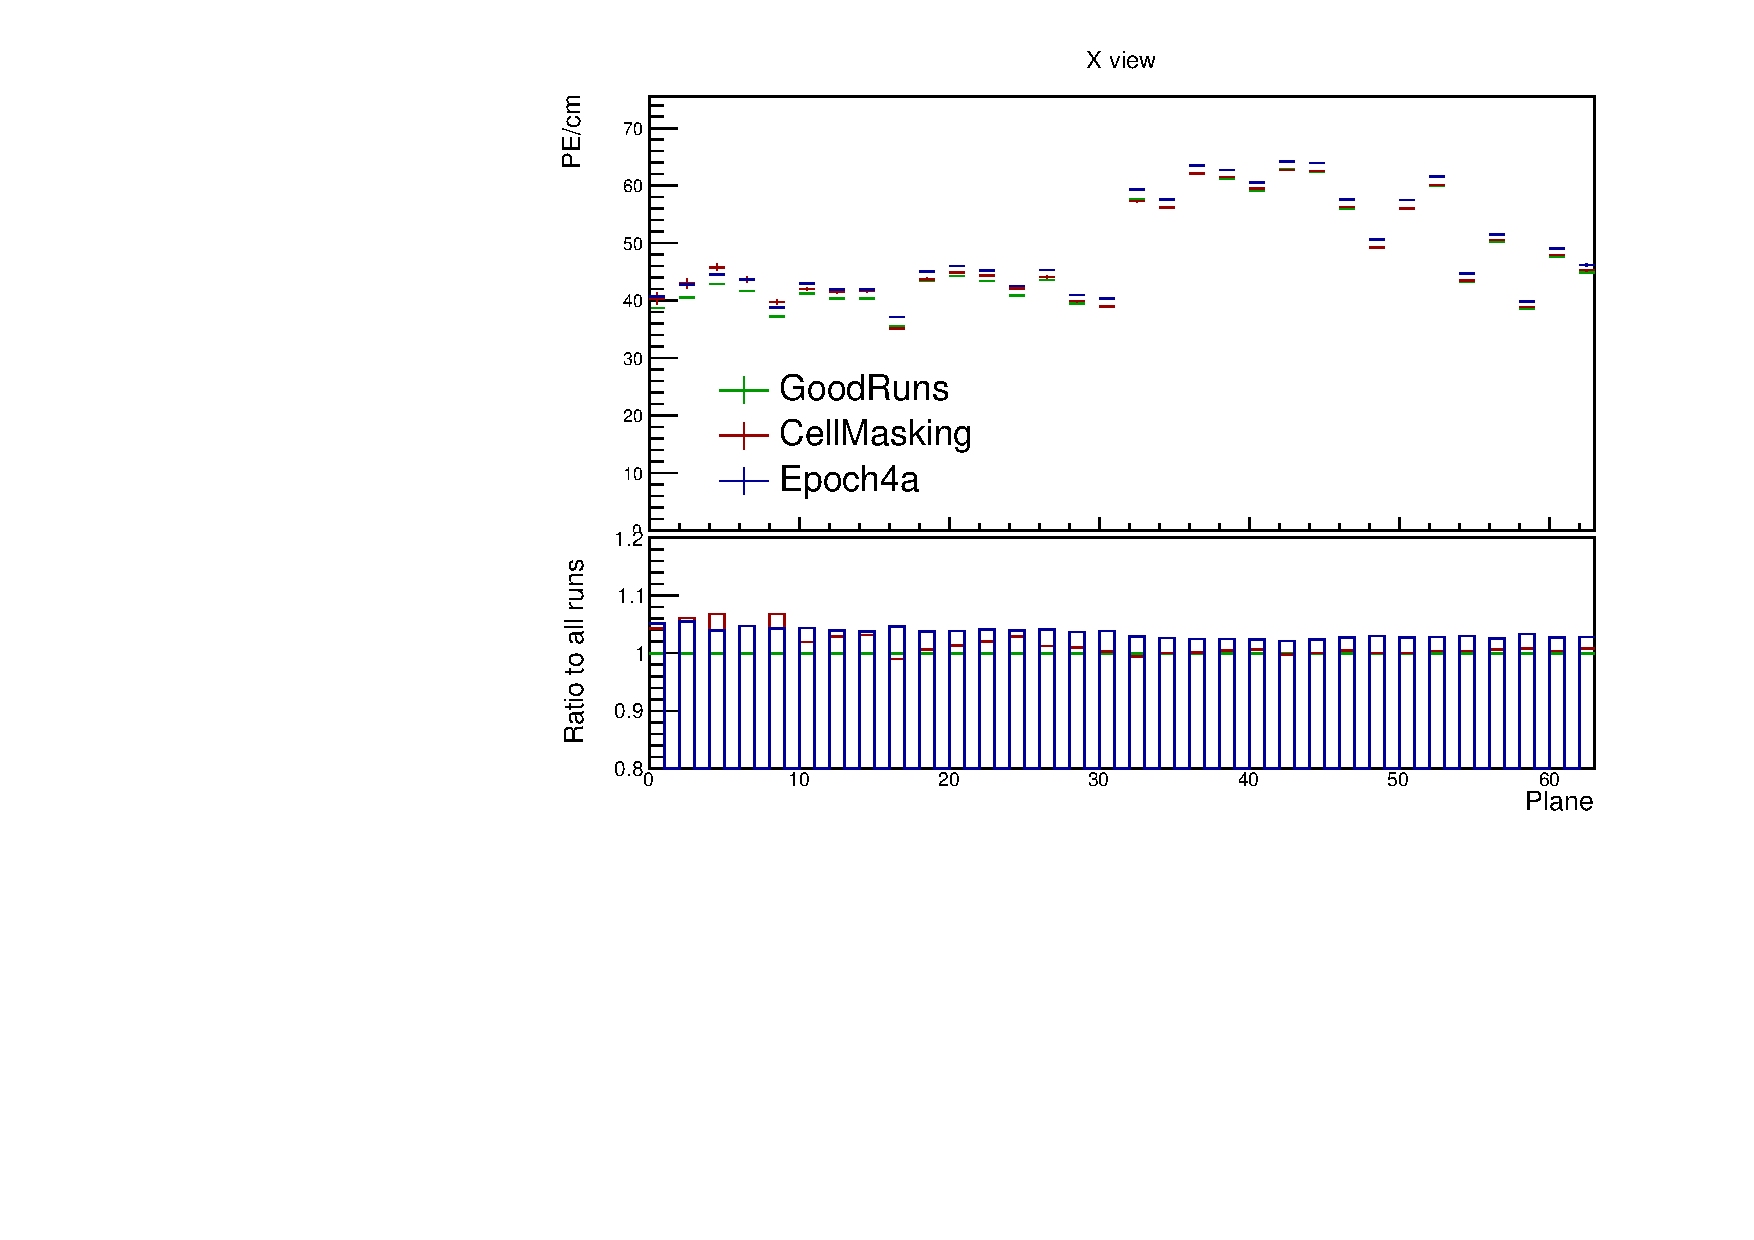
\includegraphics[width=\textwidth]{Plots/Attenprofs_P4Data_PlanePE_X_Combined.pdf}
\end{subfigure}
\begin{subfigure}[b]{\textwidth}
\centering
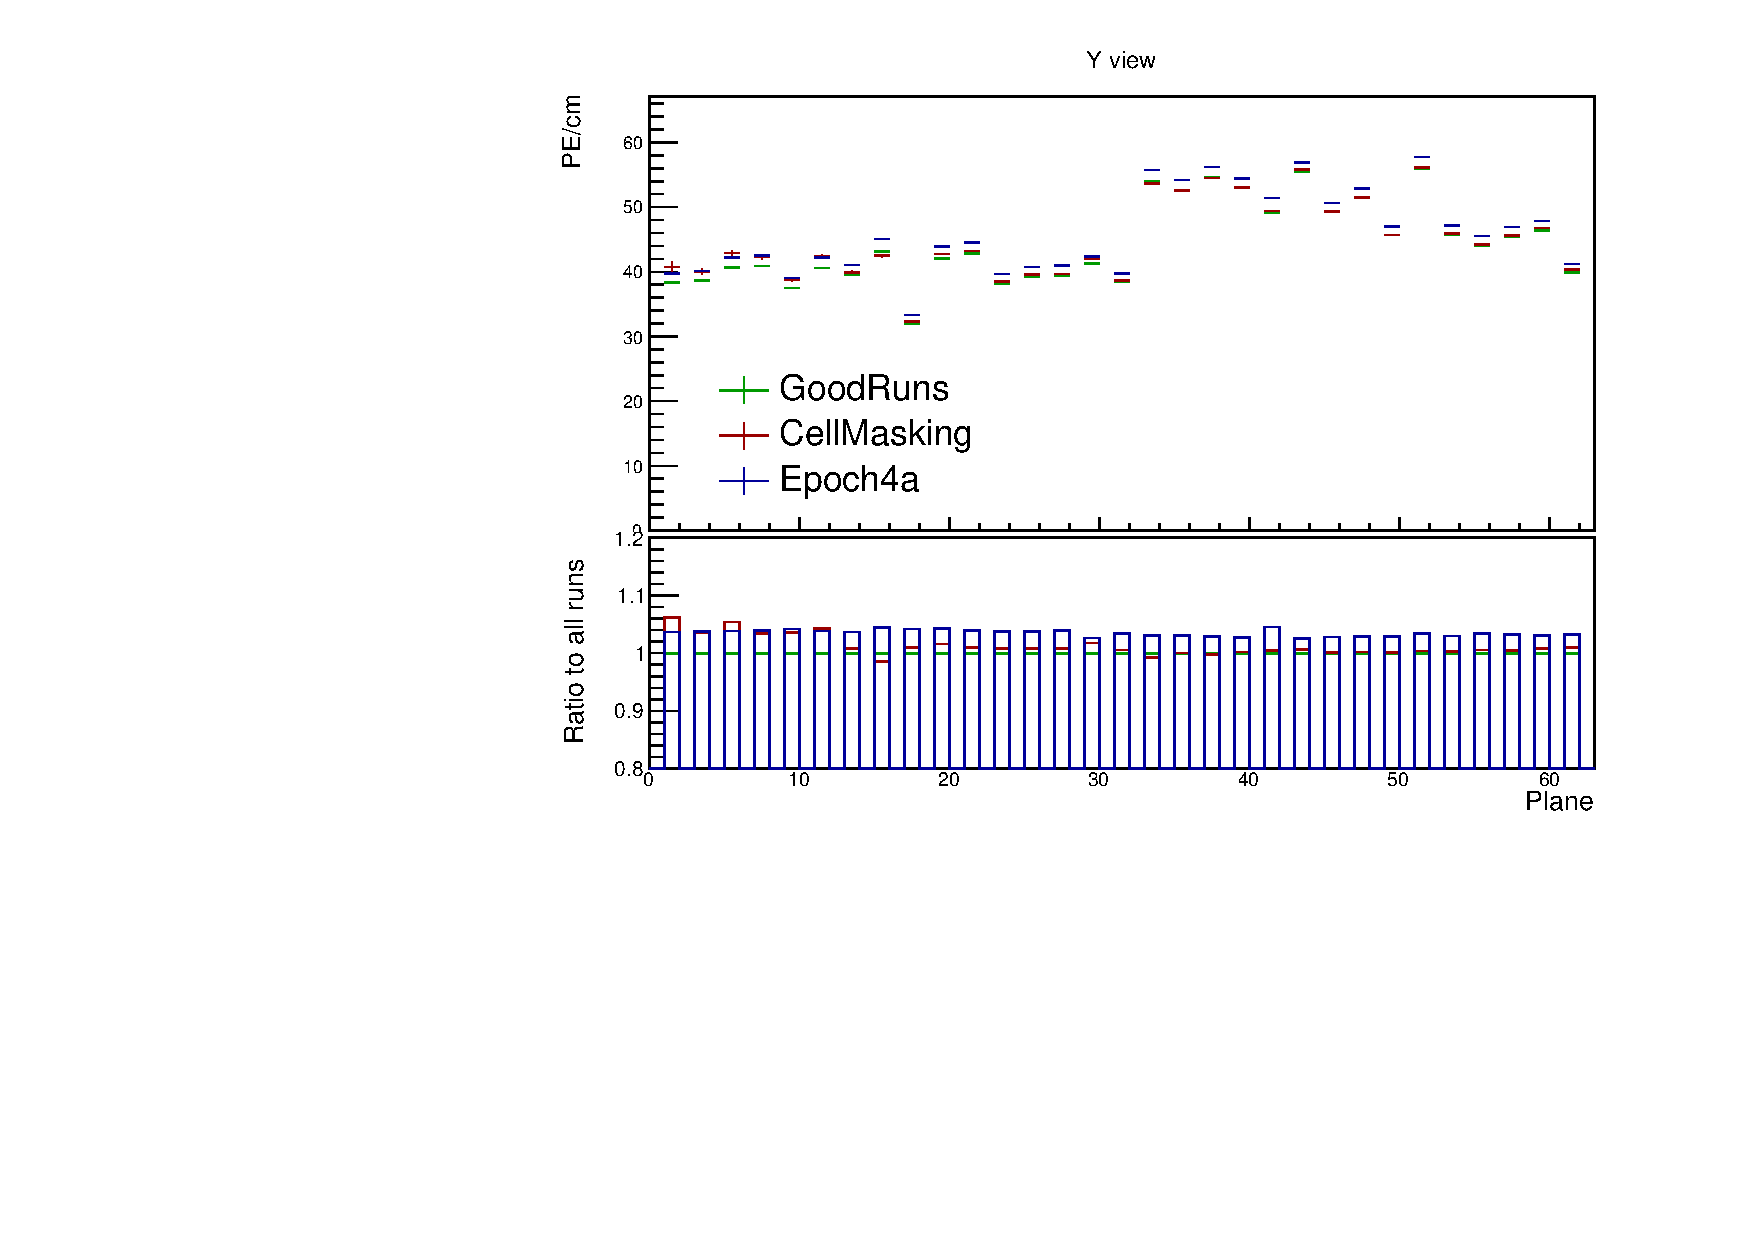
\includegraphics[width=\textwidth]{Plots/Attenprofs_P4Data_PlanePE_Y_Combined.pdf}
\end{subfigure}
\caption{Uncorrected average energy response as a function of planes for epochs in period 4.}
\label{figCalibhistPlanePE_period4}
\end{figure}

\subsubsection{Relative calibration results}

\begin{figure}[!hbtp]
\centering
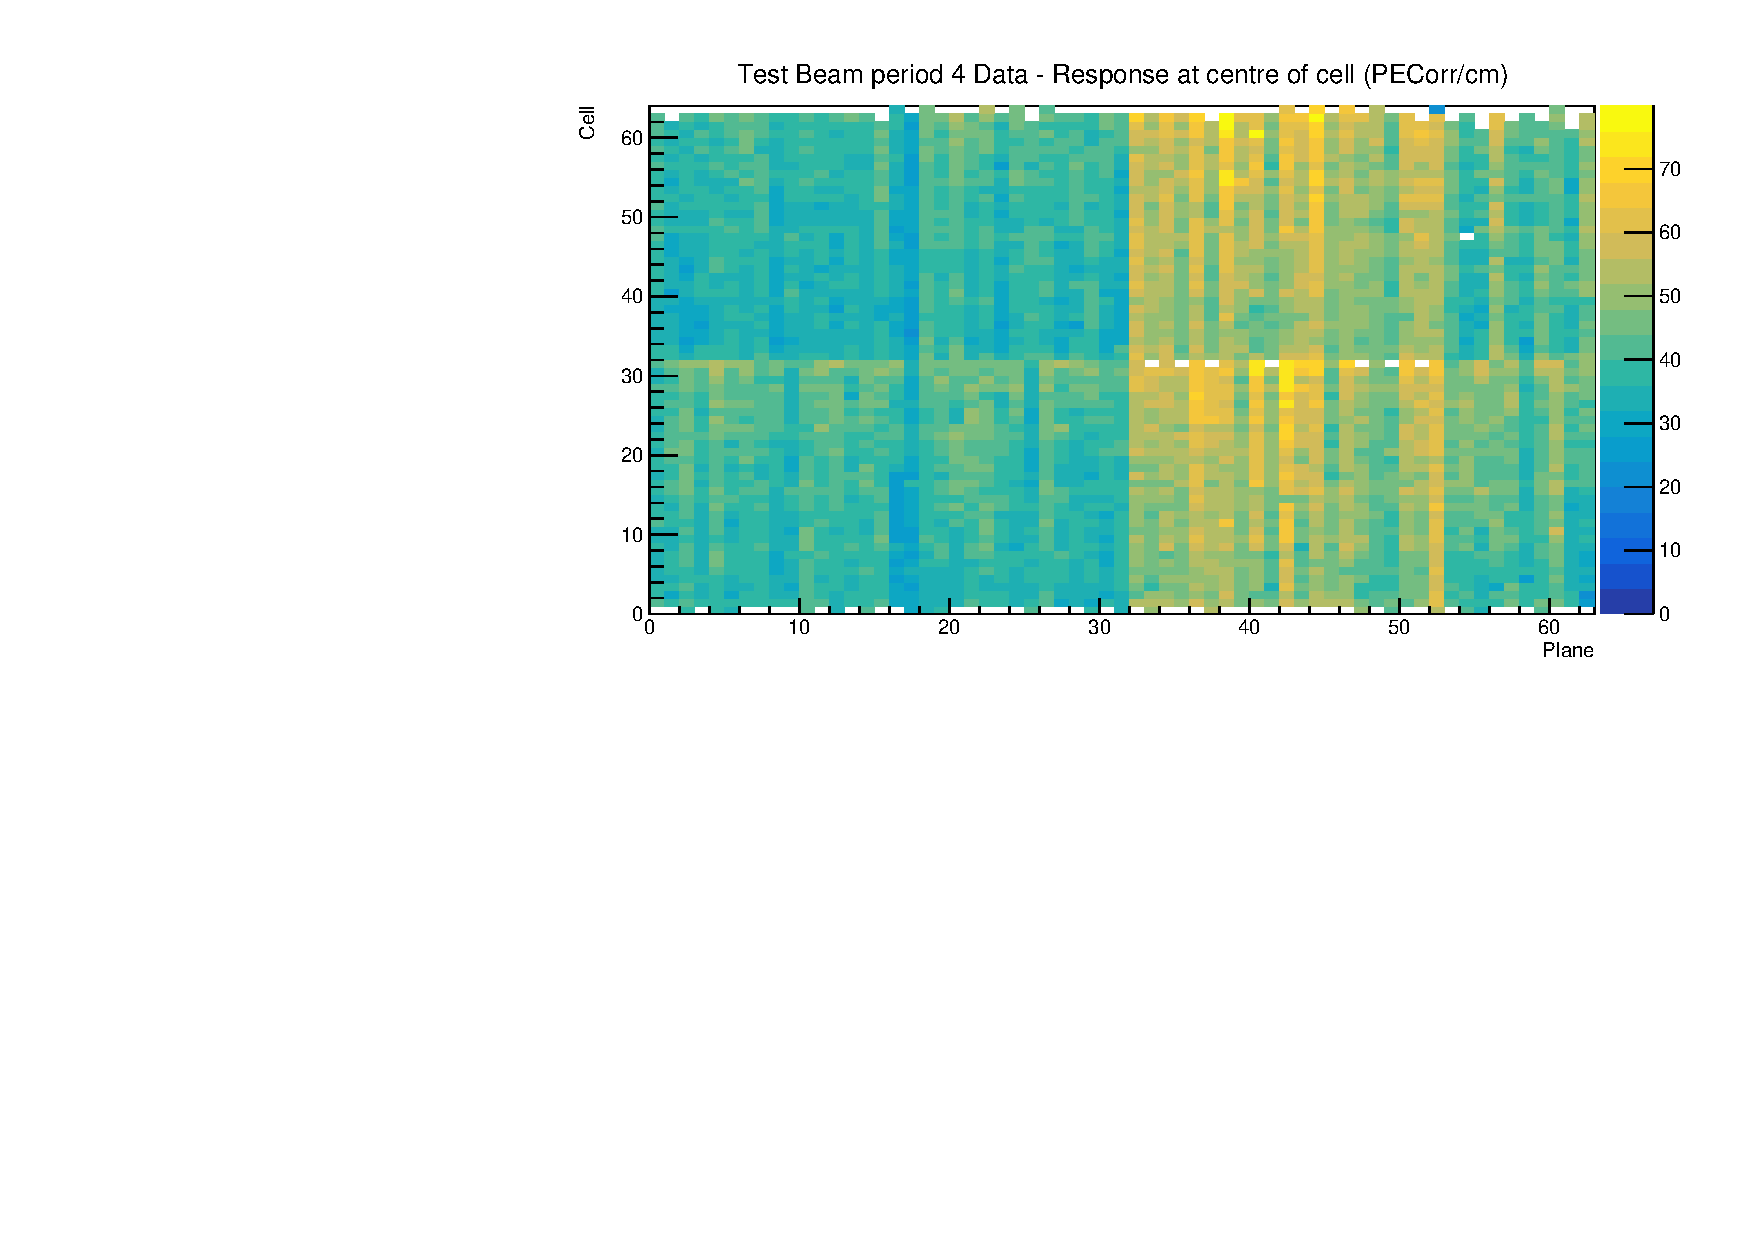
\includegraphics[width=\textwidth]{Plots/CellResponseAtCentre_period4.pdf}
\caption{Overview of the relative calibration results for the Teast Beam detector period 4 data. Each cell is represents the average corrected energy response (in PECorr/cm) in the centre of each cell. The blank cells are uncalibrated.}
\end{figure}

\subsection{Absolute calibration results}

Standard absolute calibration cuts: track window, flat-response W, positive pe, pecorr, and pathlenght reco\begin{center}
\begin{table}[h!]
\begin{tabular}{ |c|c|c|c|c|c|c|c|c|}

\hline
Sample & NHits$ x$ & MEU$ x$ & NHits$ y$ & MEU$ y$ & MEU & MEU Err & TrueE/dx & tE/dx Err\\ \hline
tb data ep3a & 2.638e+05 & 38.49 & 1.621e+06 & 39.4 & 38.94 & 0.006758 & 1.772 & 0.000238\\ \hline
tb data ep3d & 1.049e+05 & 38.63 & 6.725e+05 & 39.42 & 39.02 & 0.01048 & 1.772 & 0.000238\\ \hline
tb data p2 & 2.322e+05 & 38.7 & 1.413e+06 & 39.4 & 39.05 & 0.007252 & 1.772 & 0.000238\\ \hline
tb data p4 & 5.268e+05 & 38.63 & 3.316e+06 & 39.4 & 39.01 & 0.004703 & 1.772 & 0.000238\\ \hline
tb mc & 2.829e+05 & 40.17 & 1.842e+06 & 39.93 & 40.05 & 0.006418 & 1.772 & 0.000238\\ \hline
\end{tabular}
\label{tab:calib_summary_table}
\end{table}
\end{center}

\begin{figure}[h!]
  \begin{subfigure}{\textwidth}
  \centering
    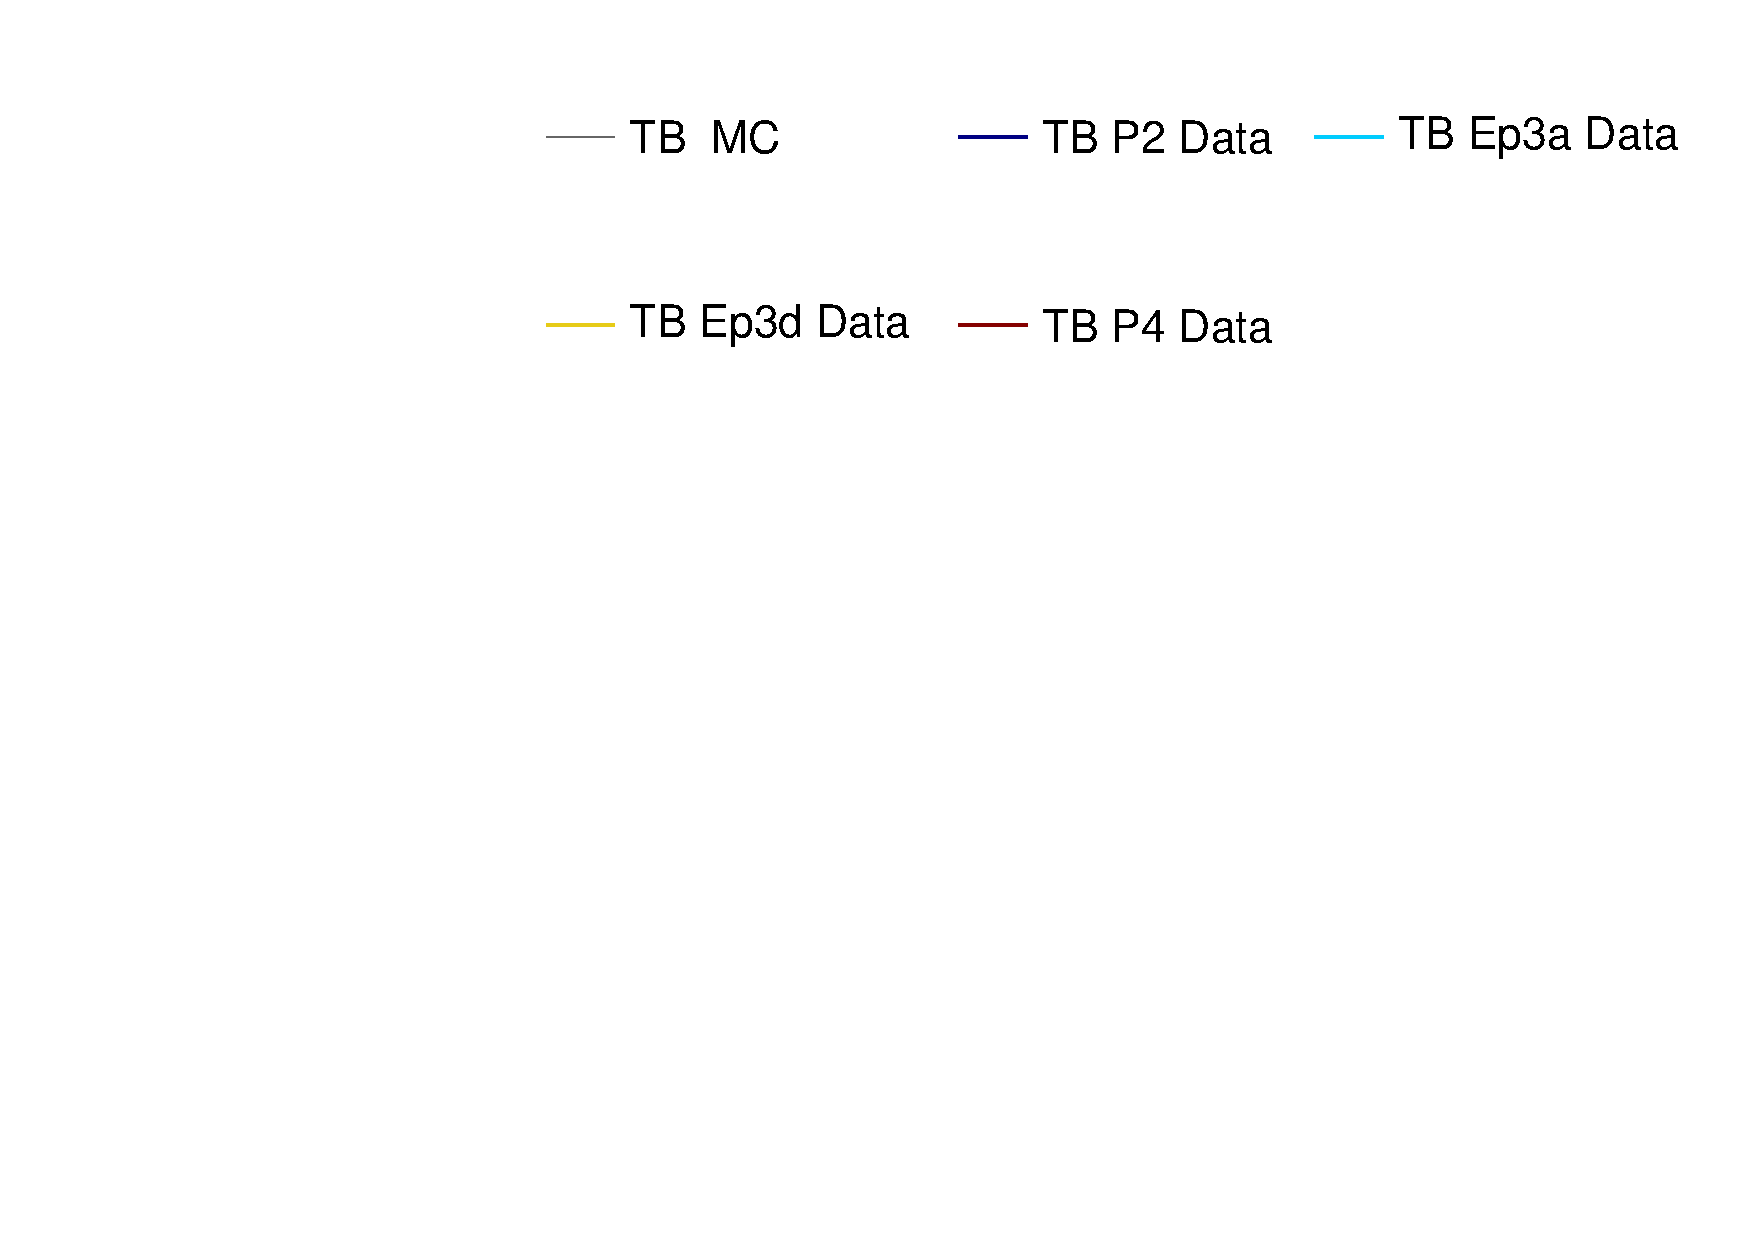
\includegraphics[height=0.2\linewidth]{essentialsec_tb/legend.pdf}
  \end{subfigure}
  \vspace*{2mm}
  
  \begin{subfigure}{0.5\textwidth}
    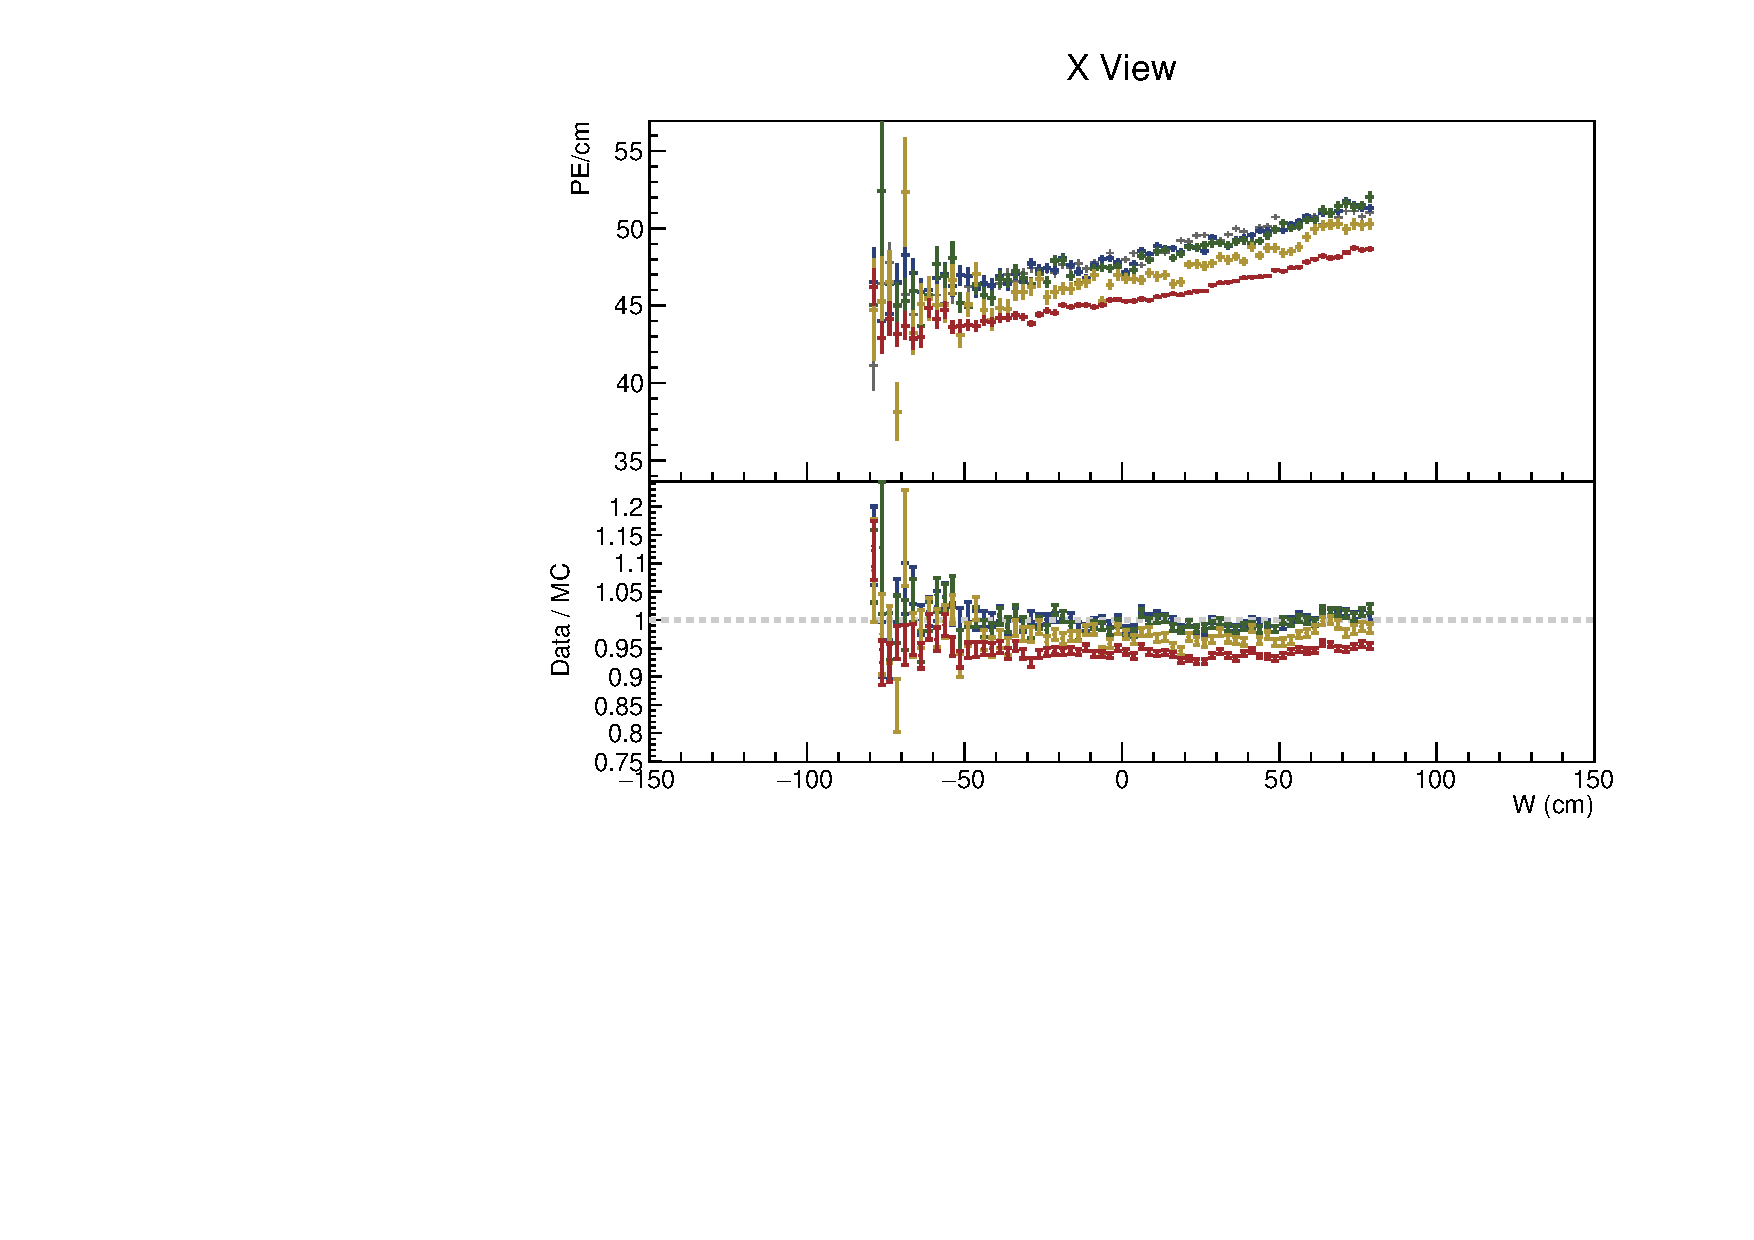
\includegraphics[width=\linewidth]{essentialsec_tb/pecm_w_x.pdf}
  \end{subfigure}
  \begin{subfigure}{0.5\textwidth}
    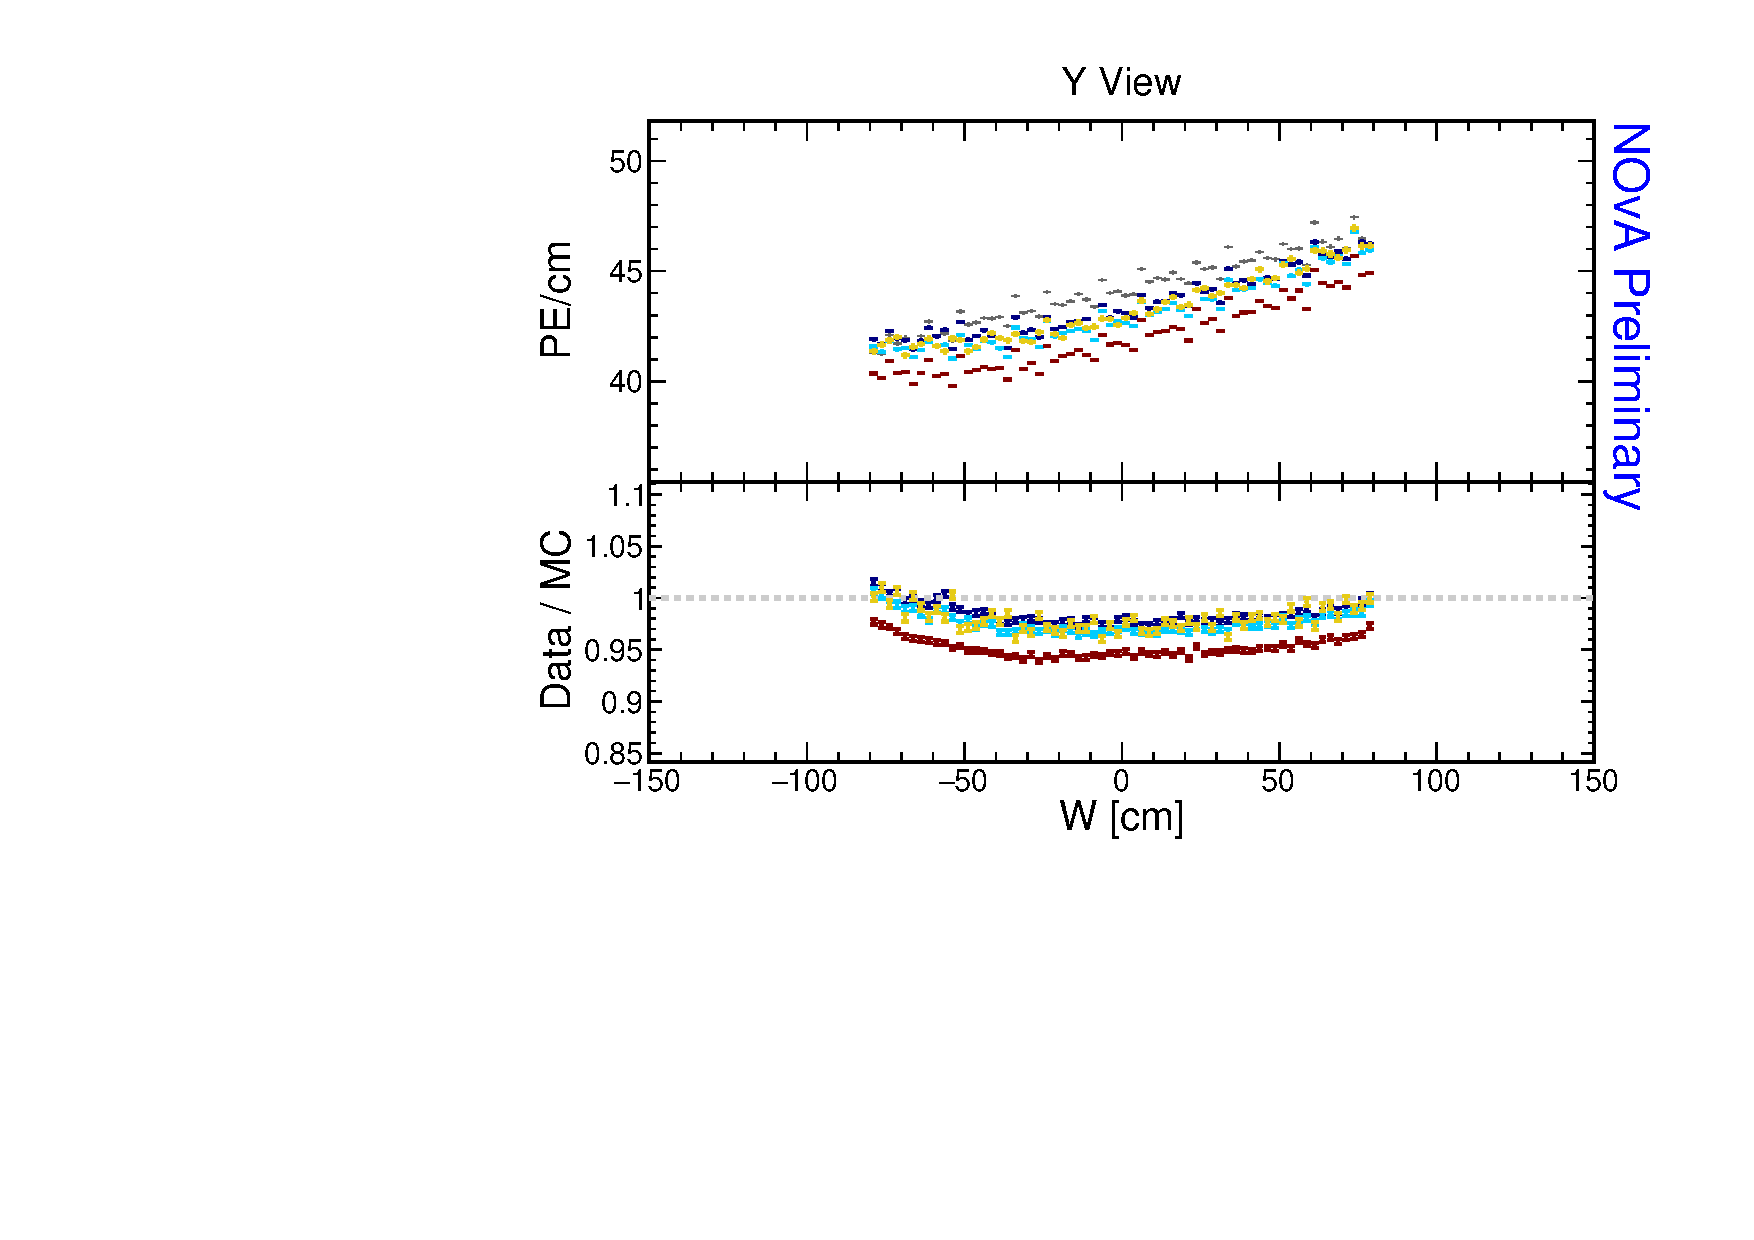
\includegraphics[width=\linewidth]{essentialsec_tb/pecm_w_y.pdf}
  \end{subfigure}
  \begin{subfigure}{0.5\textwidth}
    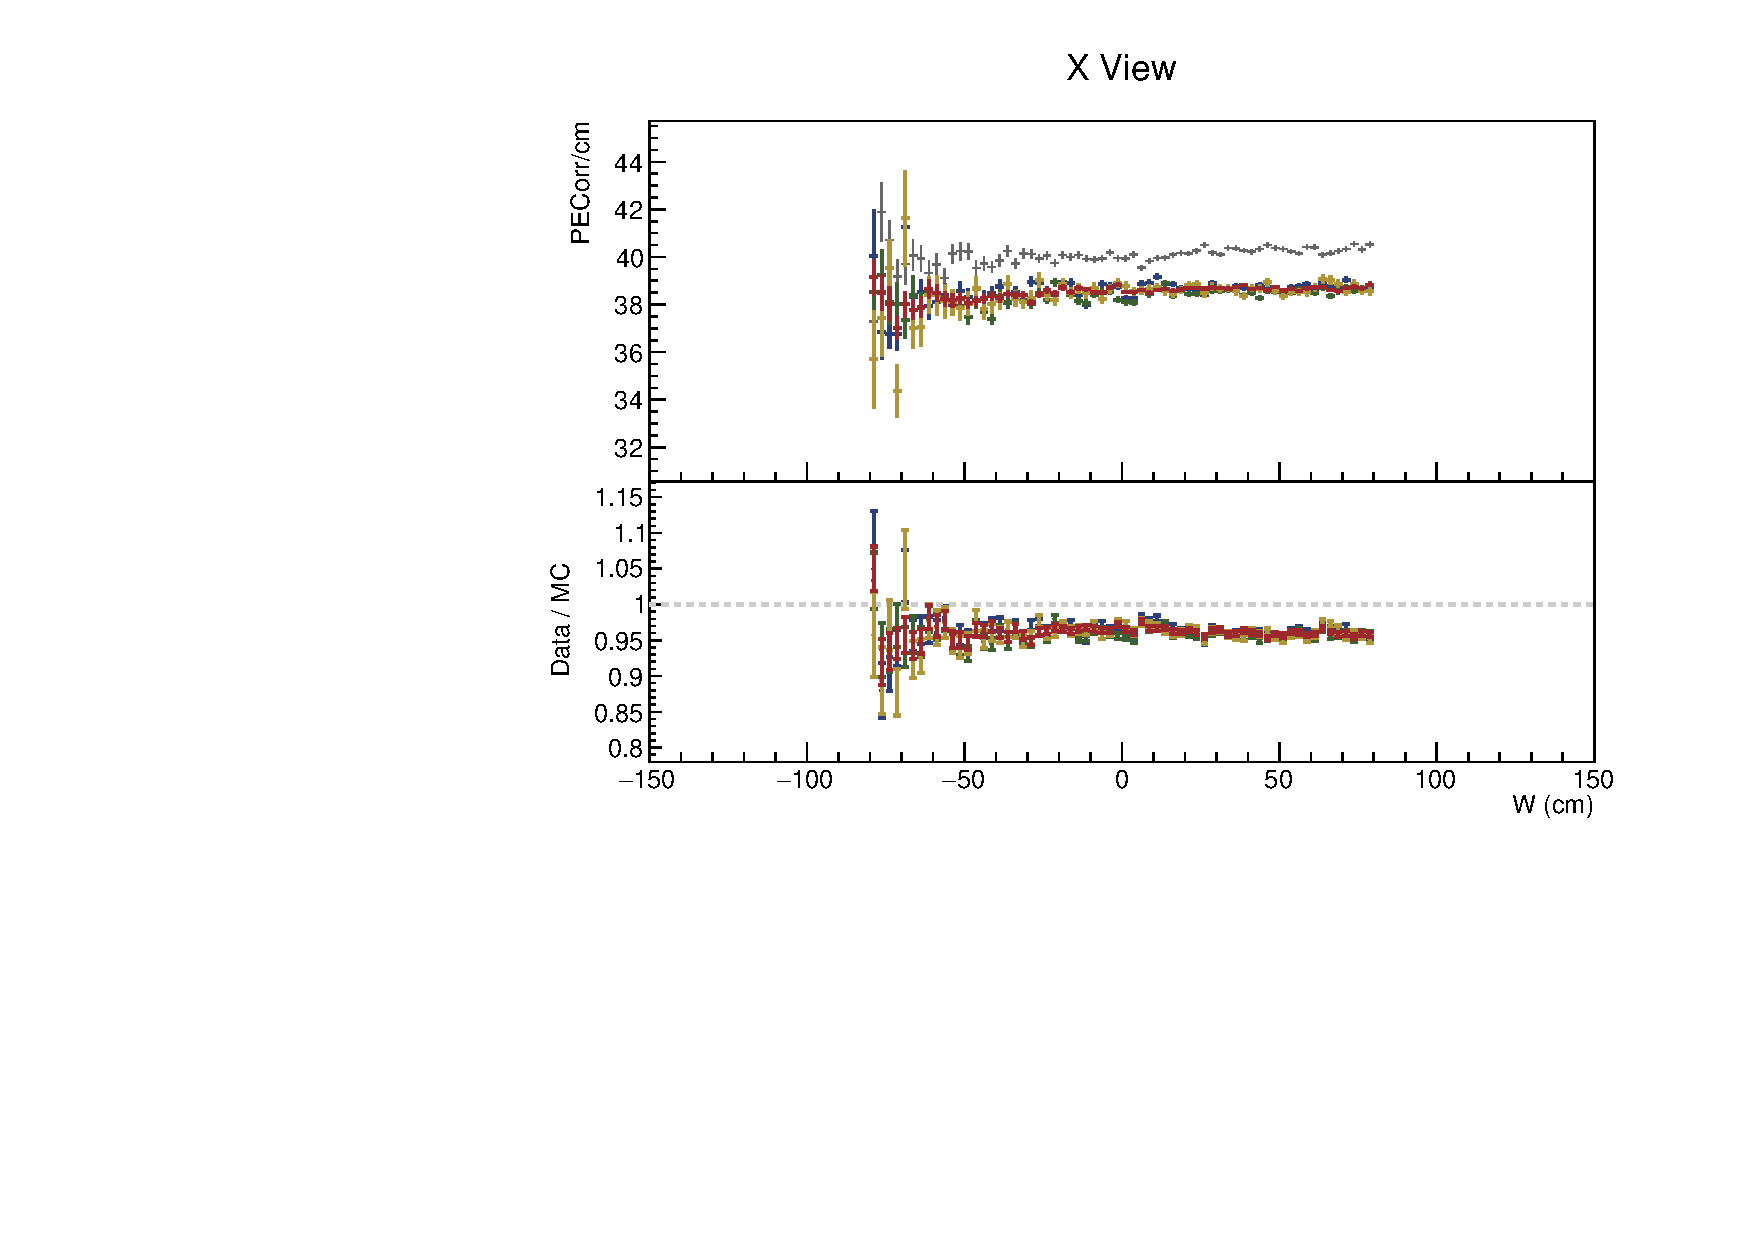
\includegraphics[width=\linewidth]{essentialsec_tb/pecorrcm_w_x.pdf}
  \end{subfigure}
  \begin{subfigure}{0.5\textwidth}
    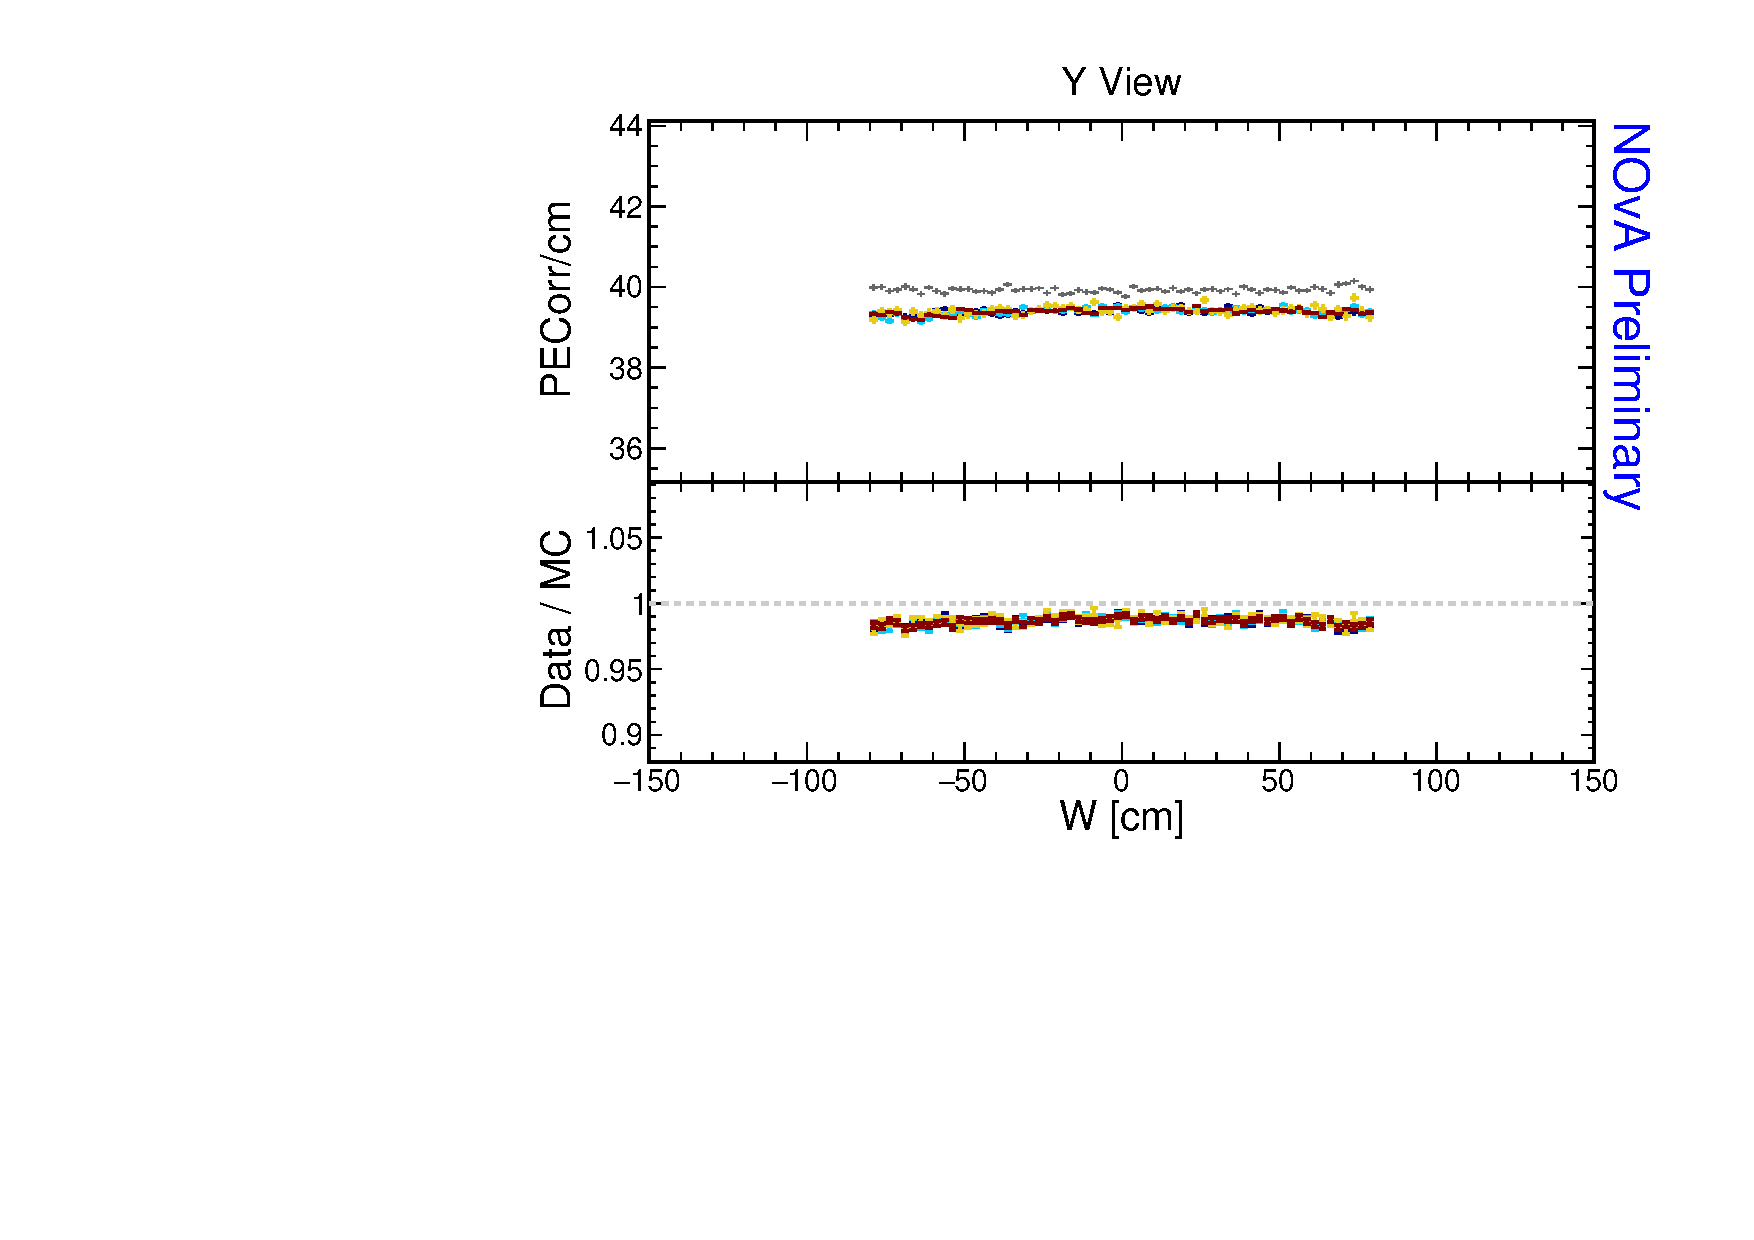
\includegraphics[width=\linewidth]{essentialsec_tb/pecorrcm_w_y.pdf}
  \end{subfigure}
  \caption{...}
  \label{figAbsCalibW1}
\end{figure}

\begin{figure}[h!]
  \begin{subfigure}{\textwidth}
  \centering
    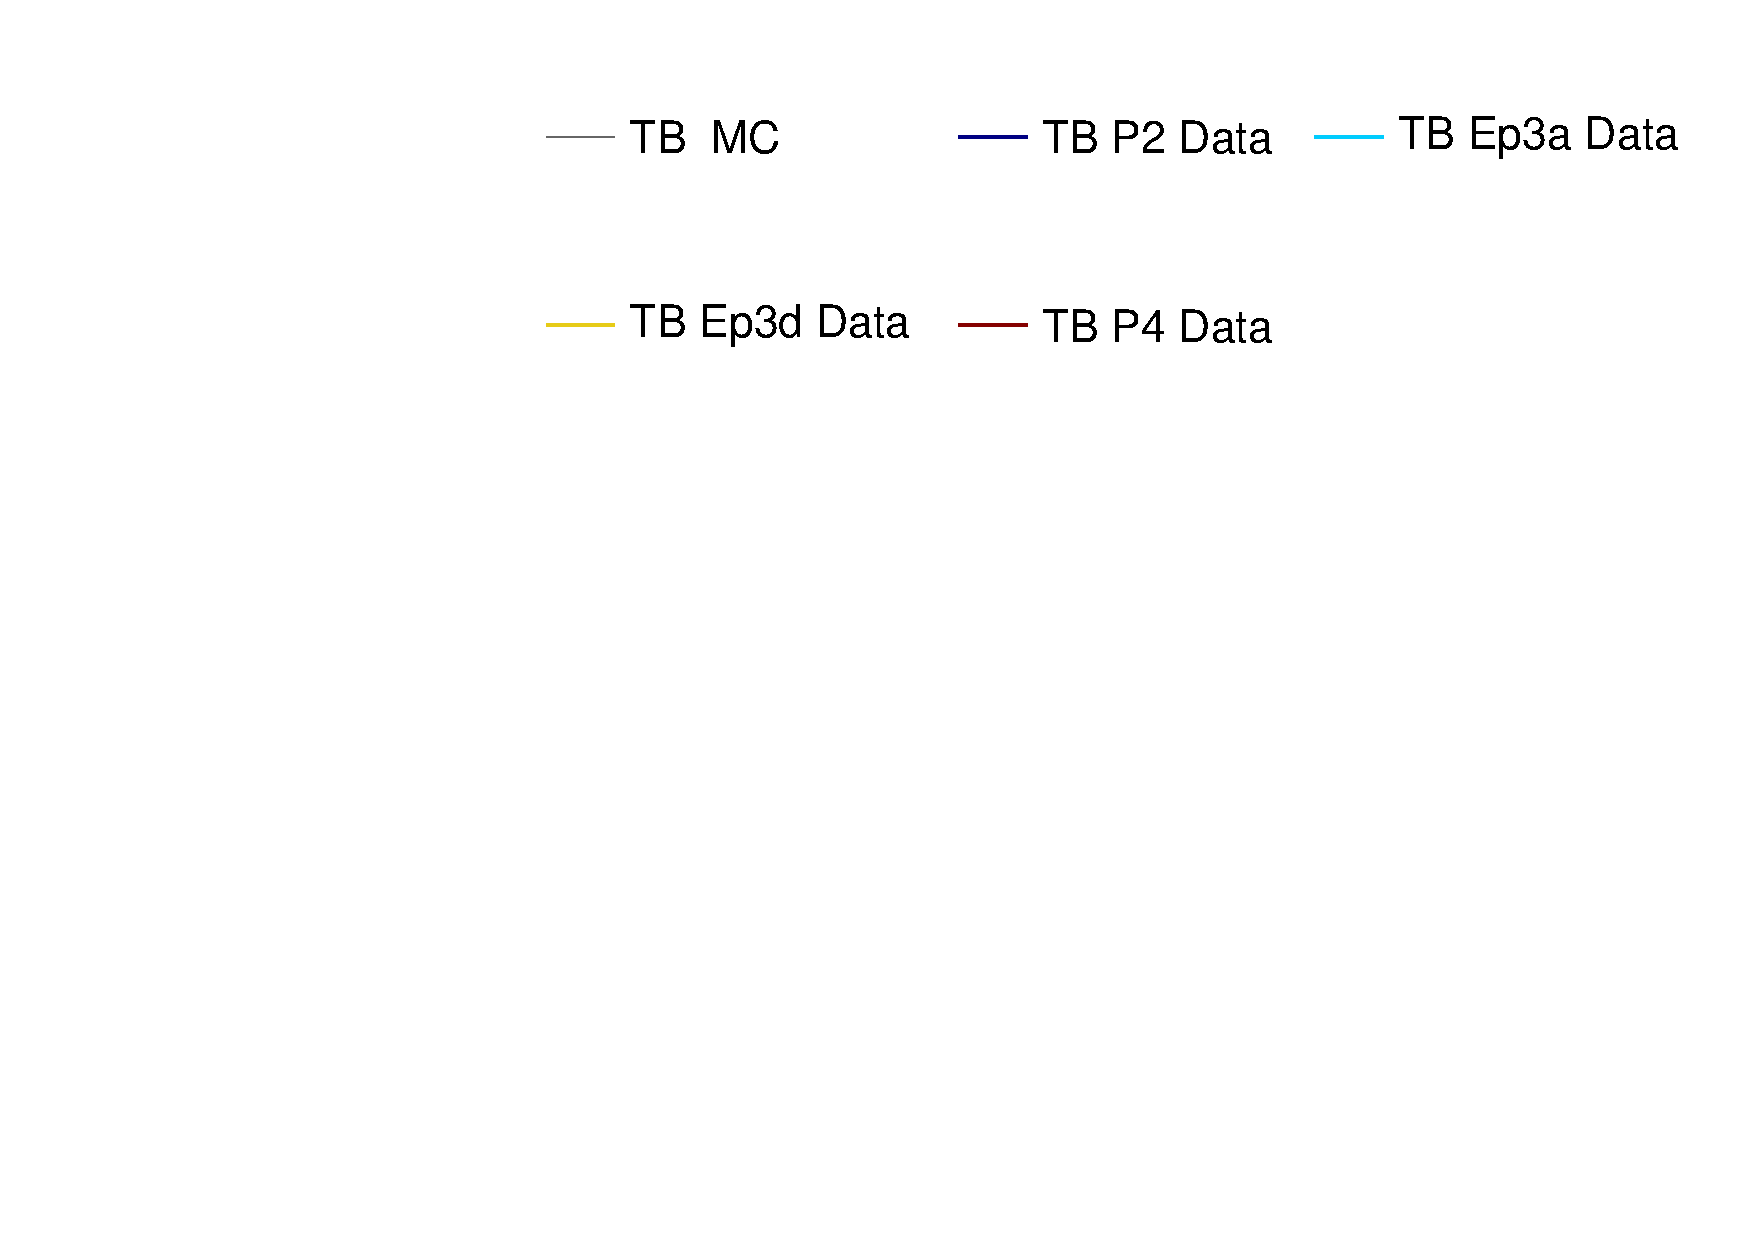
\includegraphics[height=0.2\linewidth]{essentialsec_tb/legend.pdf}
  \end{subfigure}
  \vspace*{2mm}

  \begin{subfigure}{0.5\textwidth}
    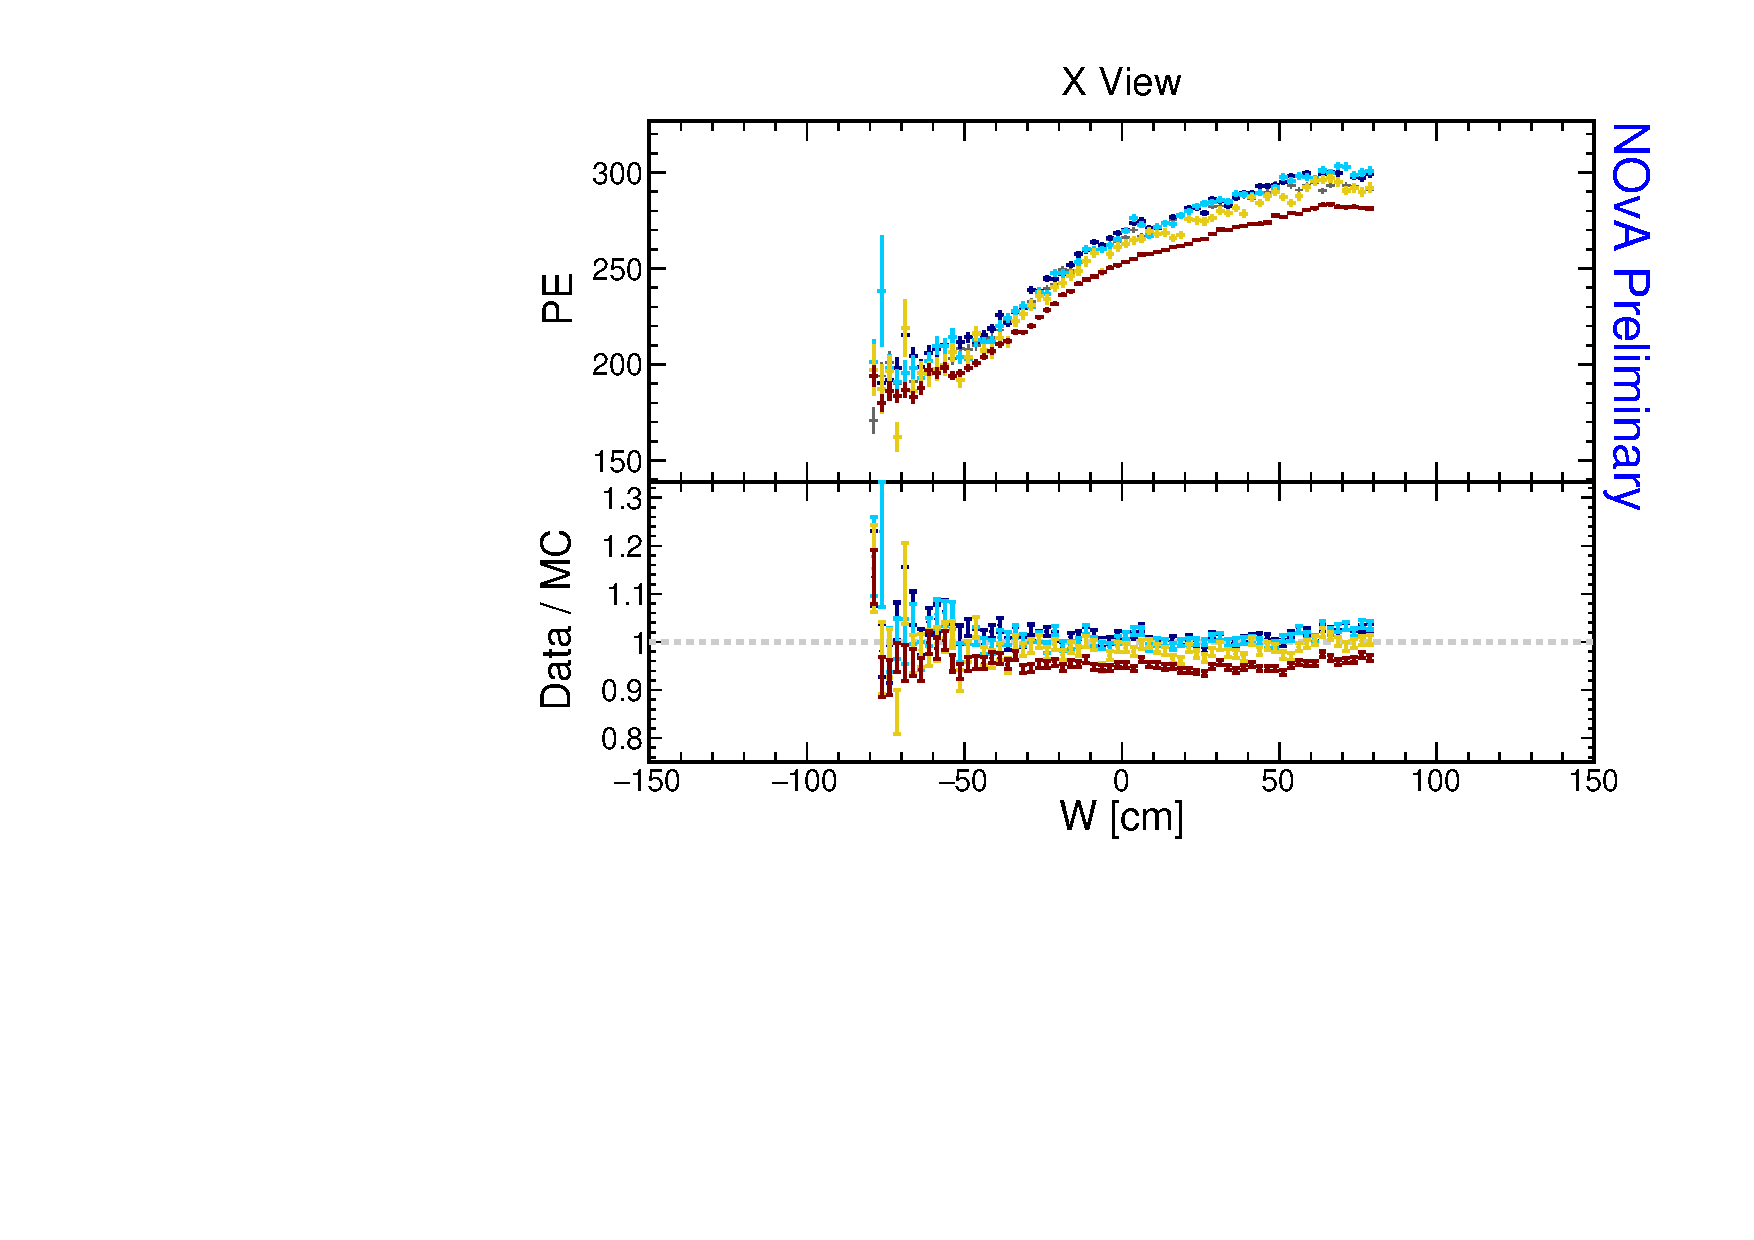
\includegraphics[width=\linewidth]{essentialsec_tb/pe_w_x.pdf}
  \end{subfigure}
  \begin{subfigure}{0.5\textwidth}
    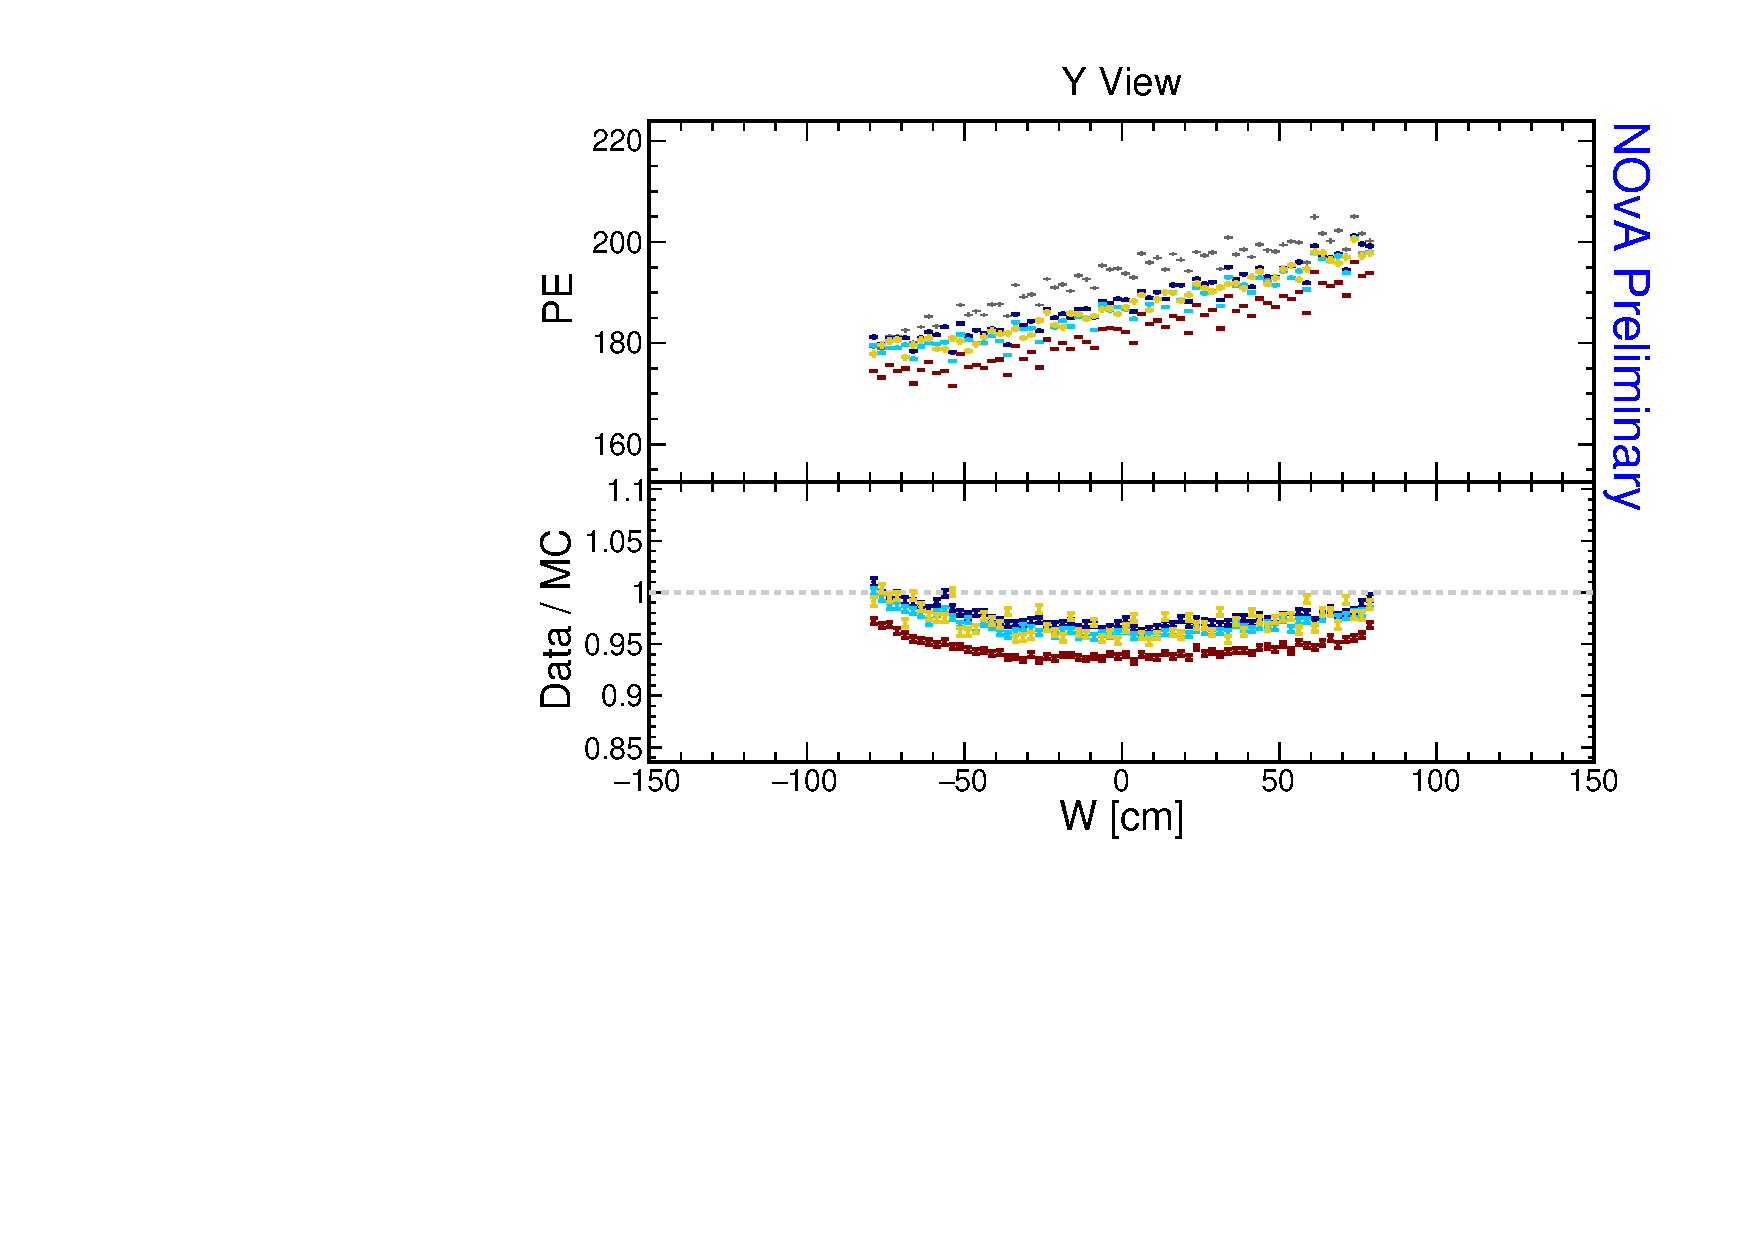
\includegraphics[width=\linewidth]{essentialsec_tb/pe_w_y.pdf}
  \end{subfigure}
  \begin{subfigure}{0.5\textwidth}
    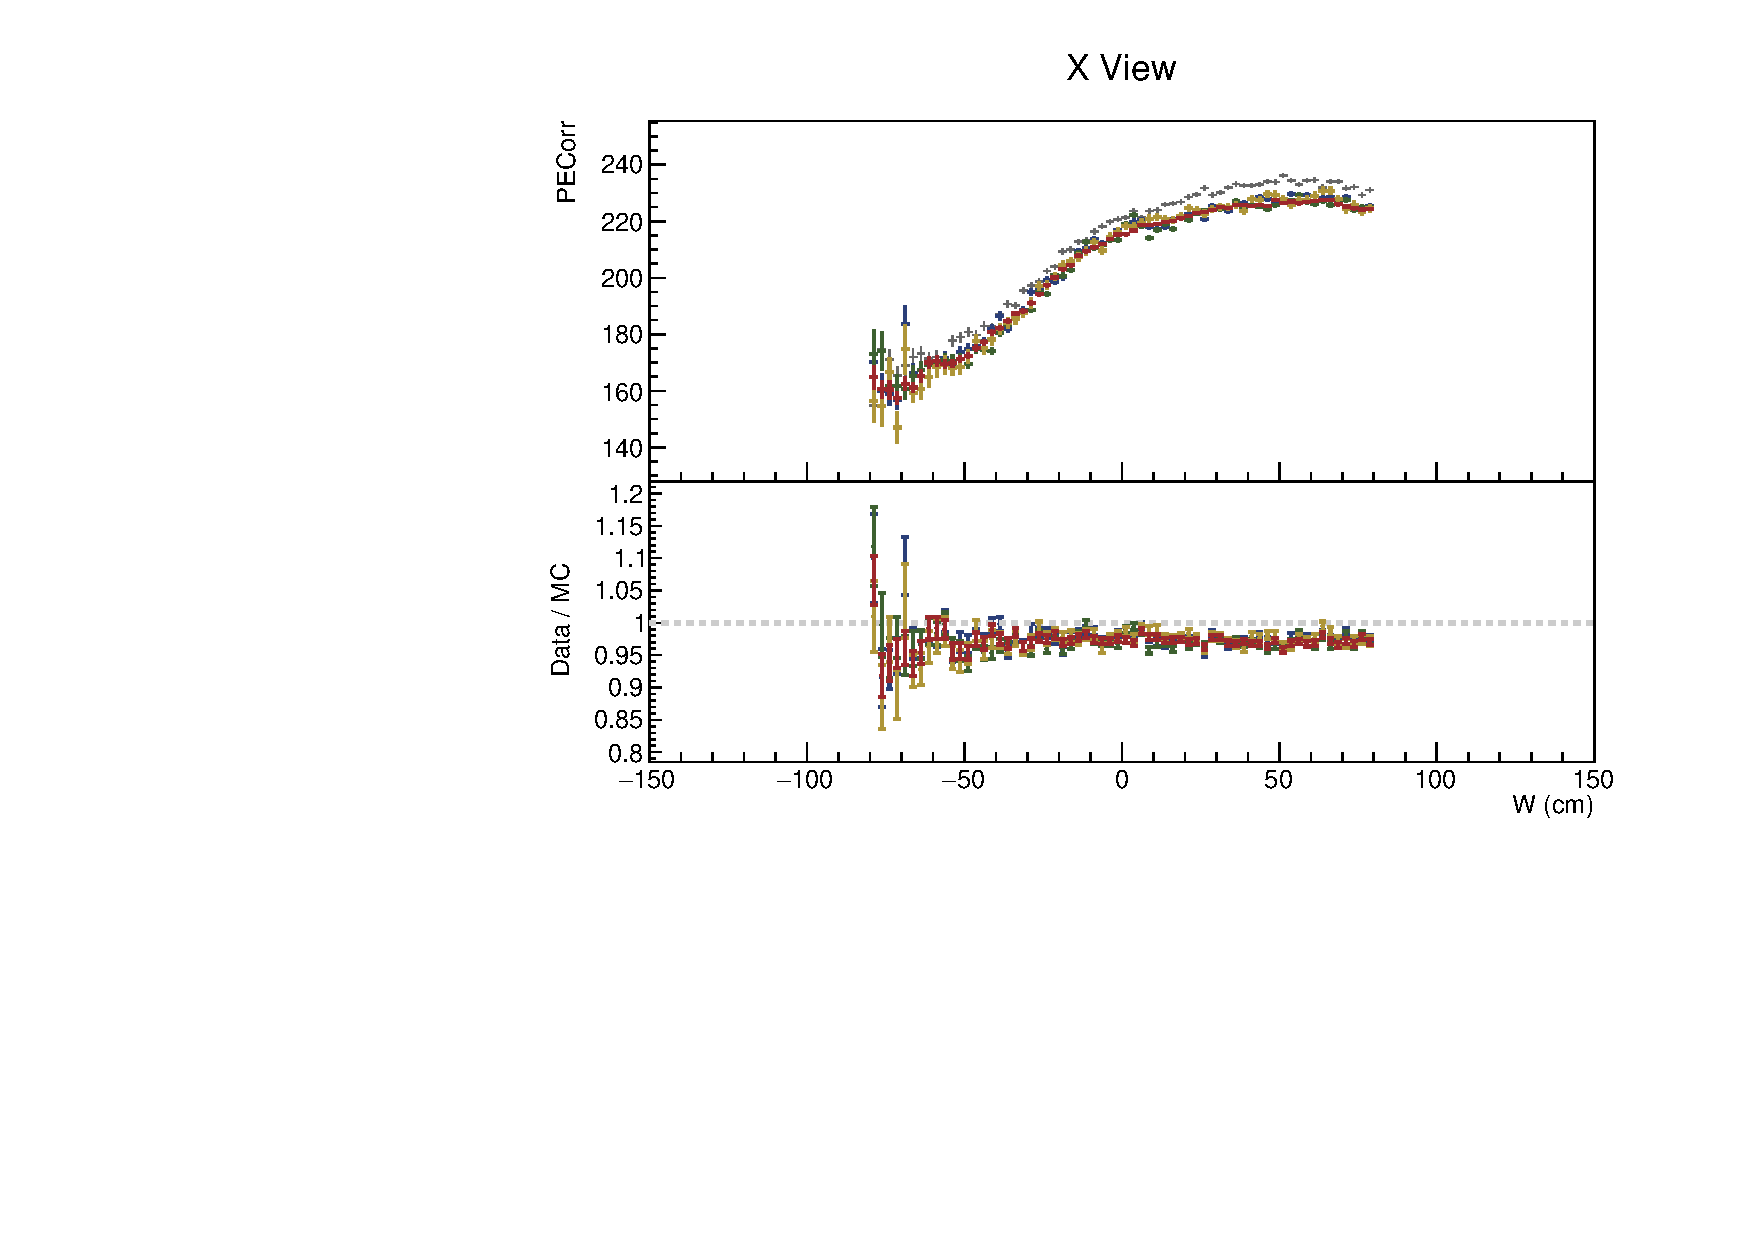
\includegraphics[width=\linewidth]{essentialsec_tb/pecorr_w_x.pdf}
  \end{subfigure}
  \begin{subfigure}{0.5\textwidth}
    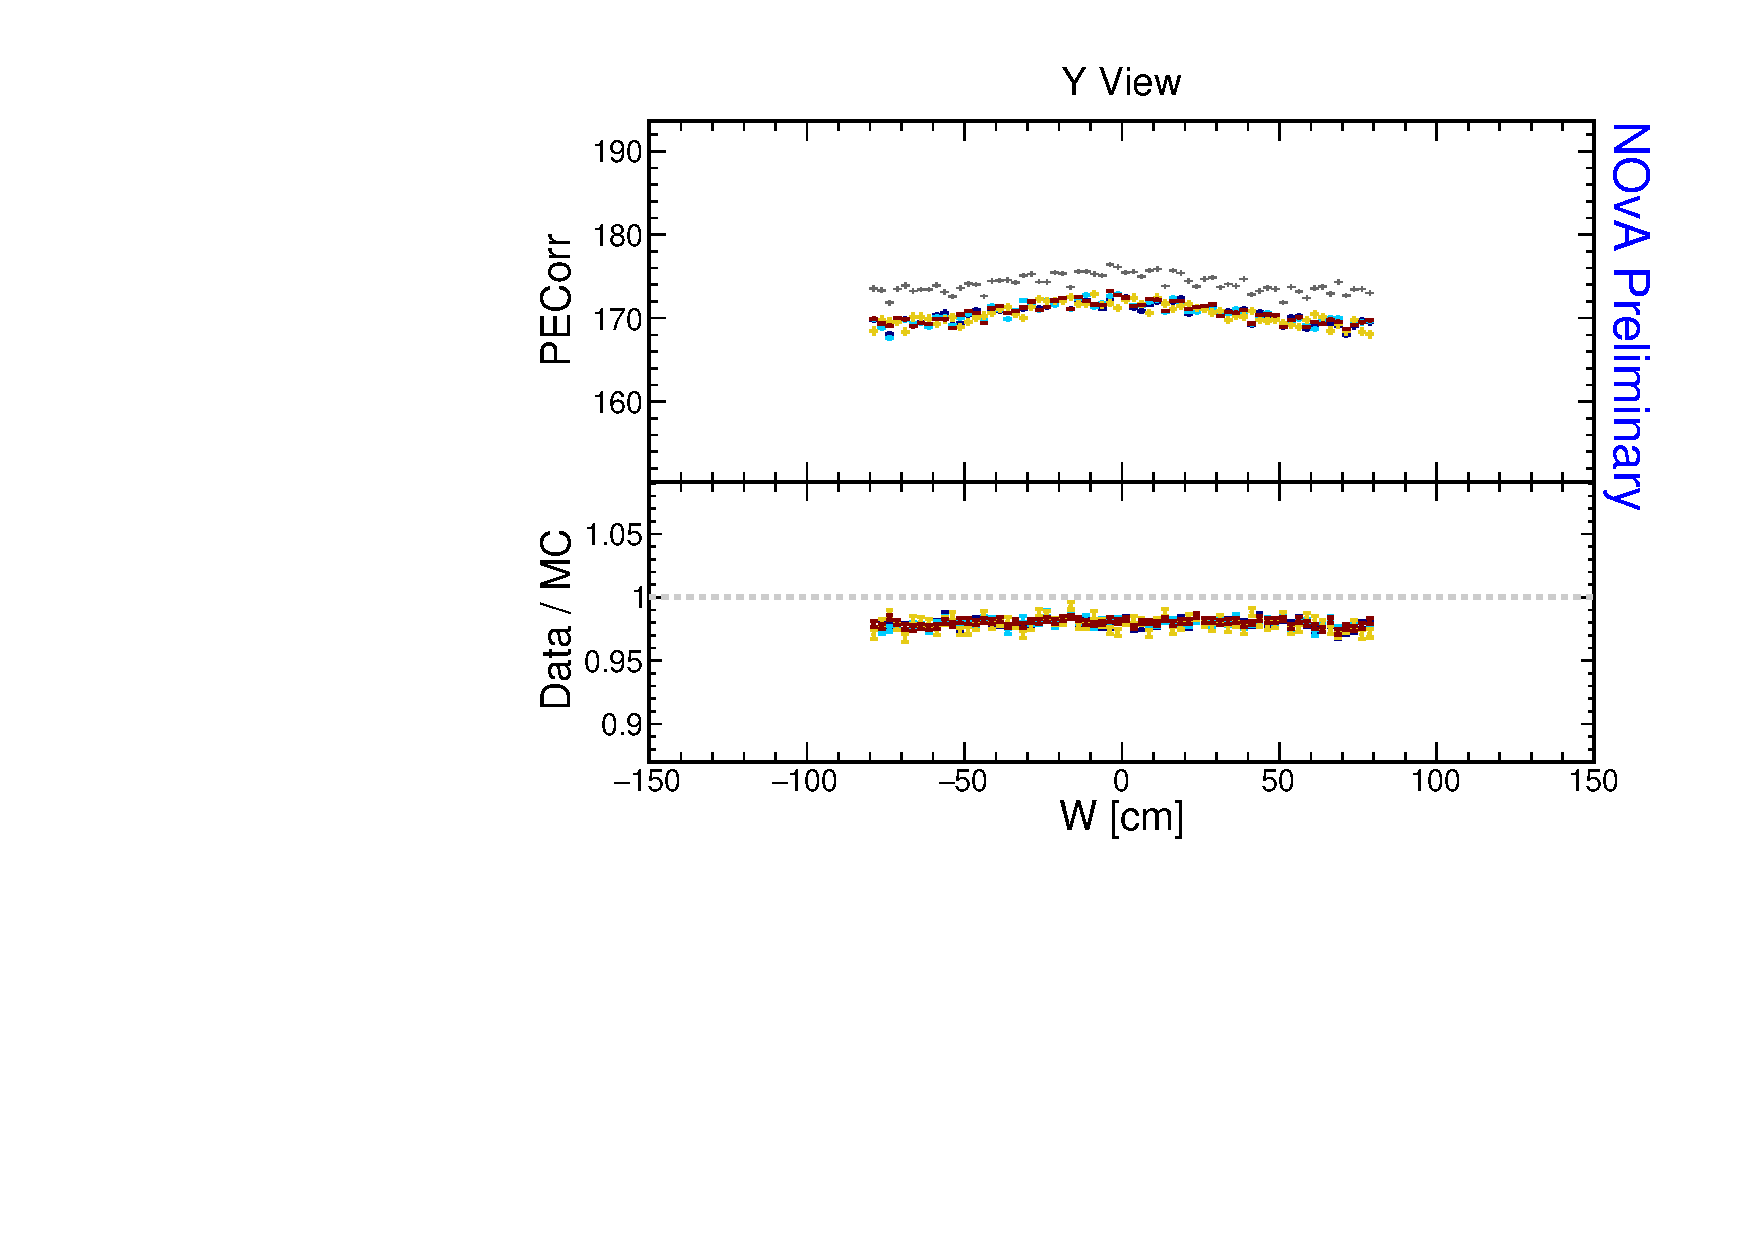
\includegraphics[width=\linewidth]{essentialsec_tb/pecorr_w_y.pdf}
  \end{subfigure}
  \begin{subfigure}{0.5\textwidth}
    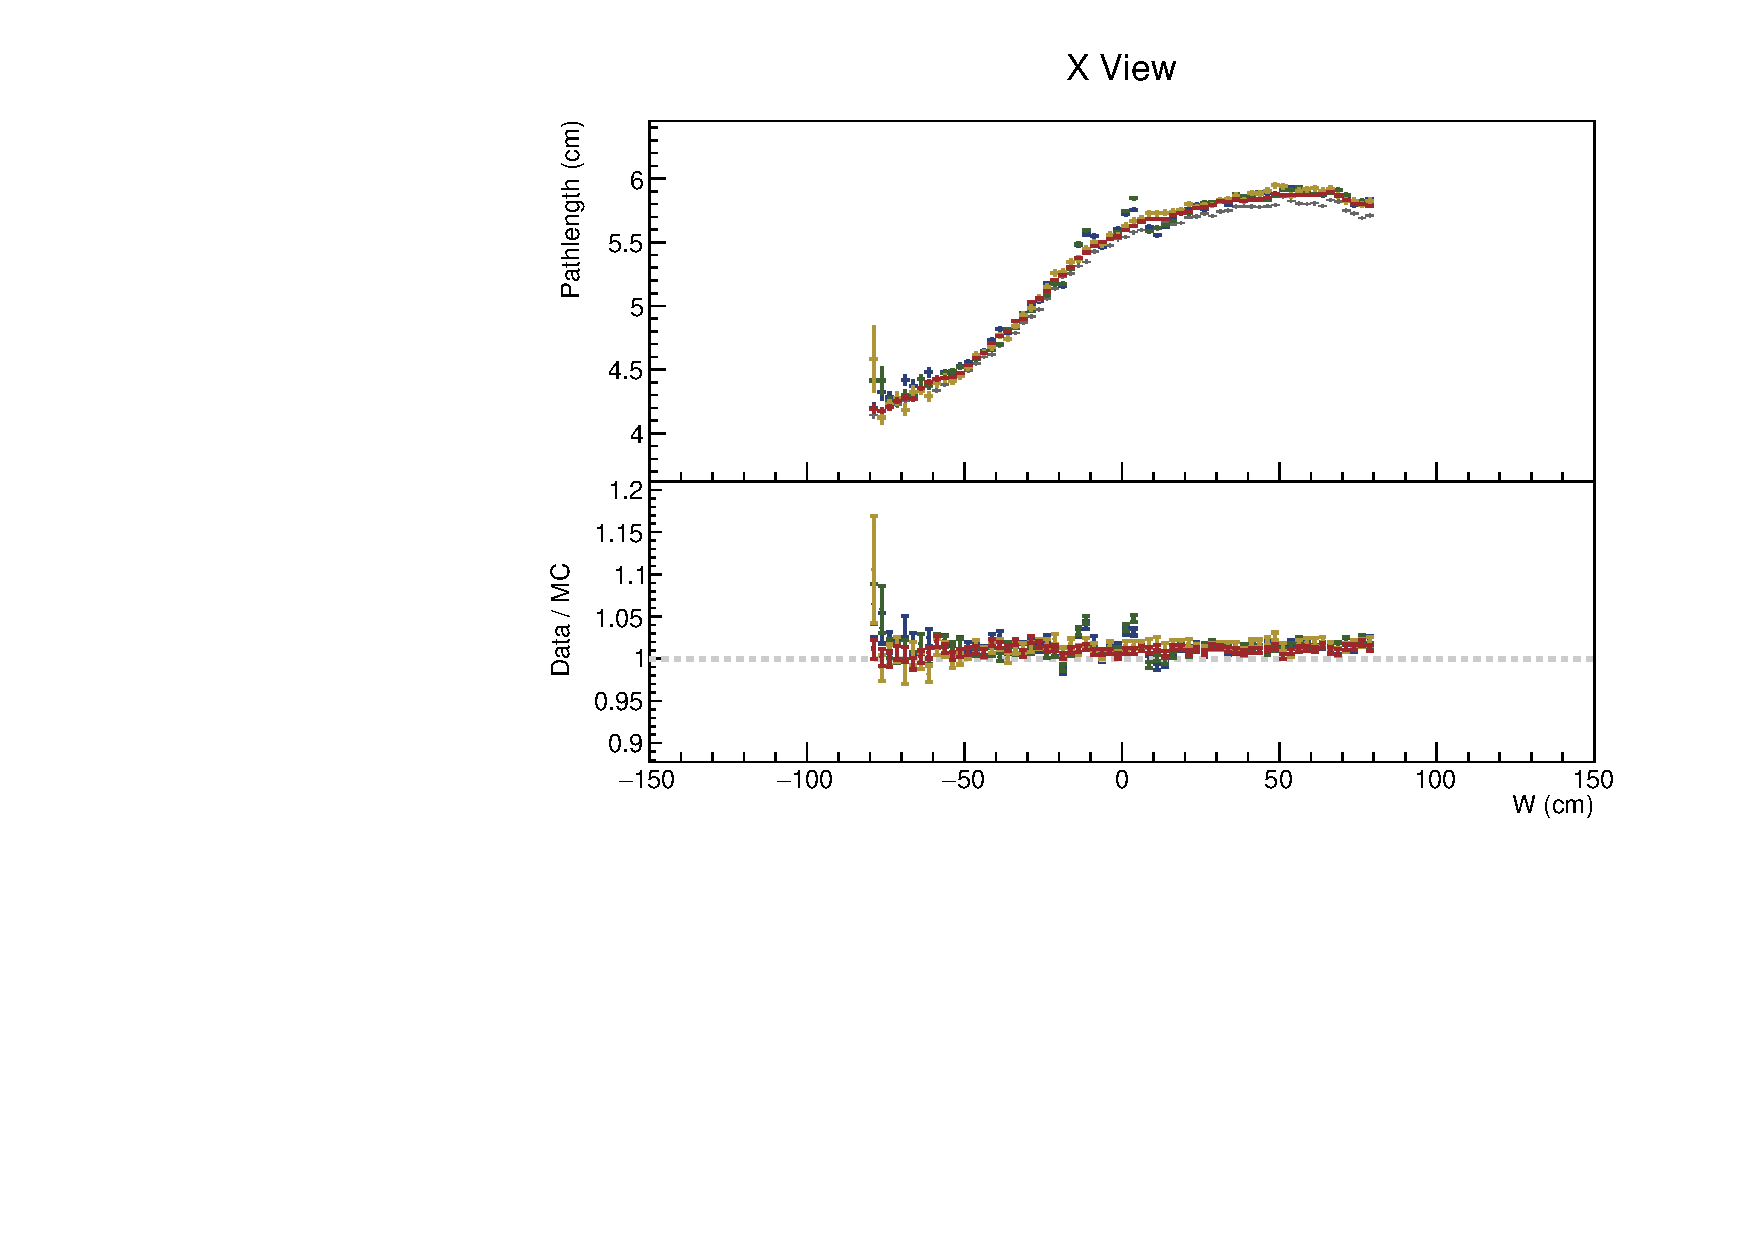
\includegraphics[width=\linewidth]{essentialsec_tb/cm_w_x.pdf}
  \end{subfigure}
  \begin{subfigure}{0.5\textwidth}
    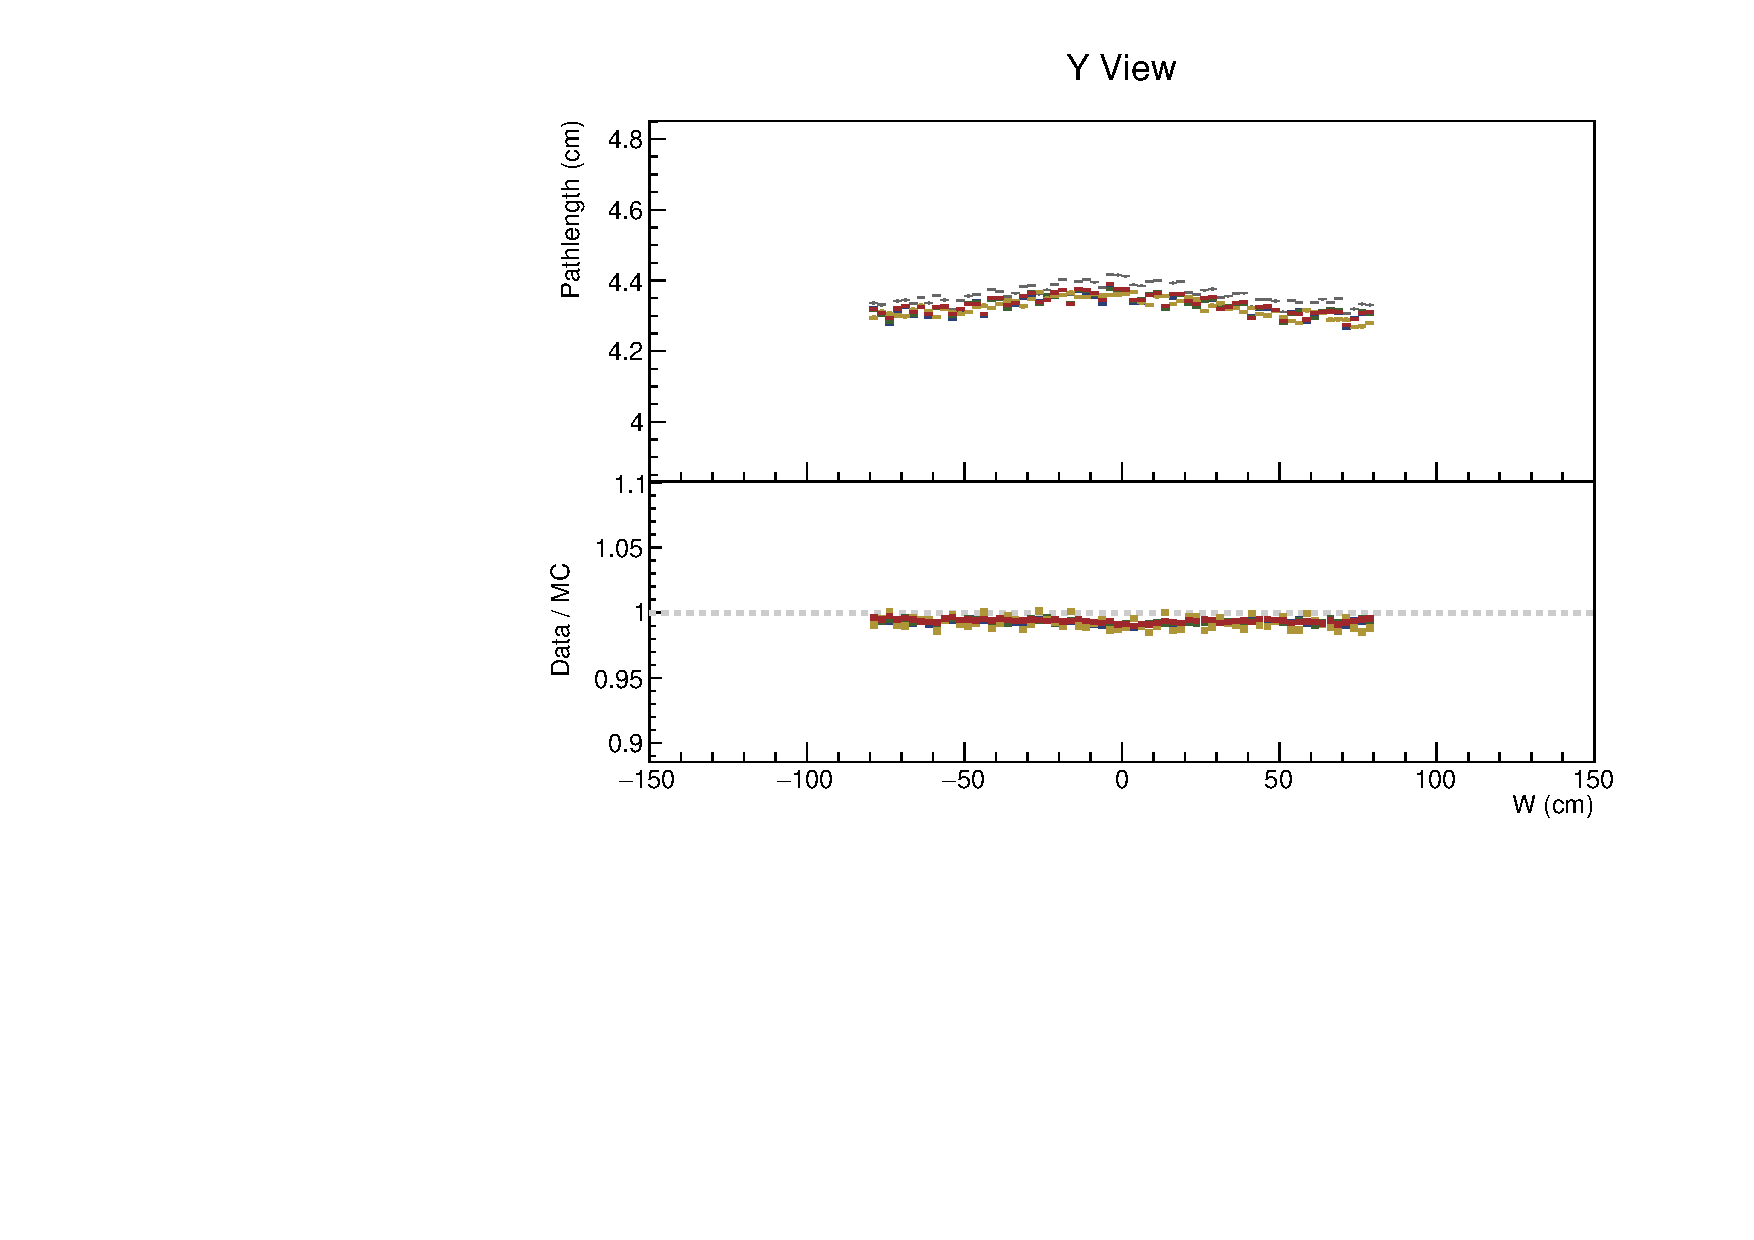
\includegraphics[width=\linewidth]{essentialsec_tb/cm_w_y.pdf}
  \end{subfigure}
  \caption{...}
  \label{figAbsCalibW2}
\end{figure}

\begin{figure}[h!]
  \begin{subfigure}{\textwidth}
  \centering
    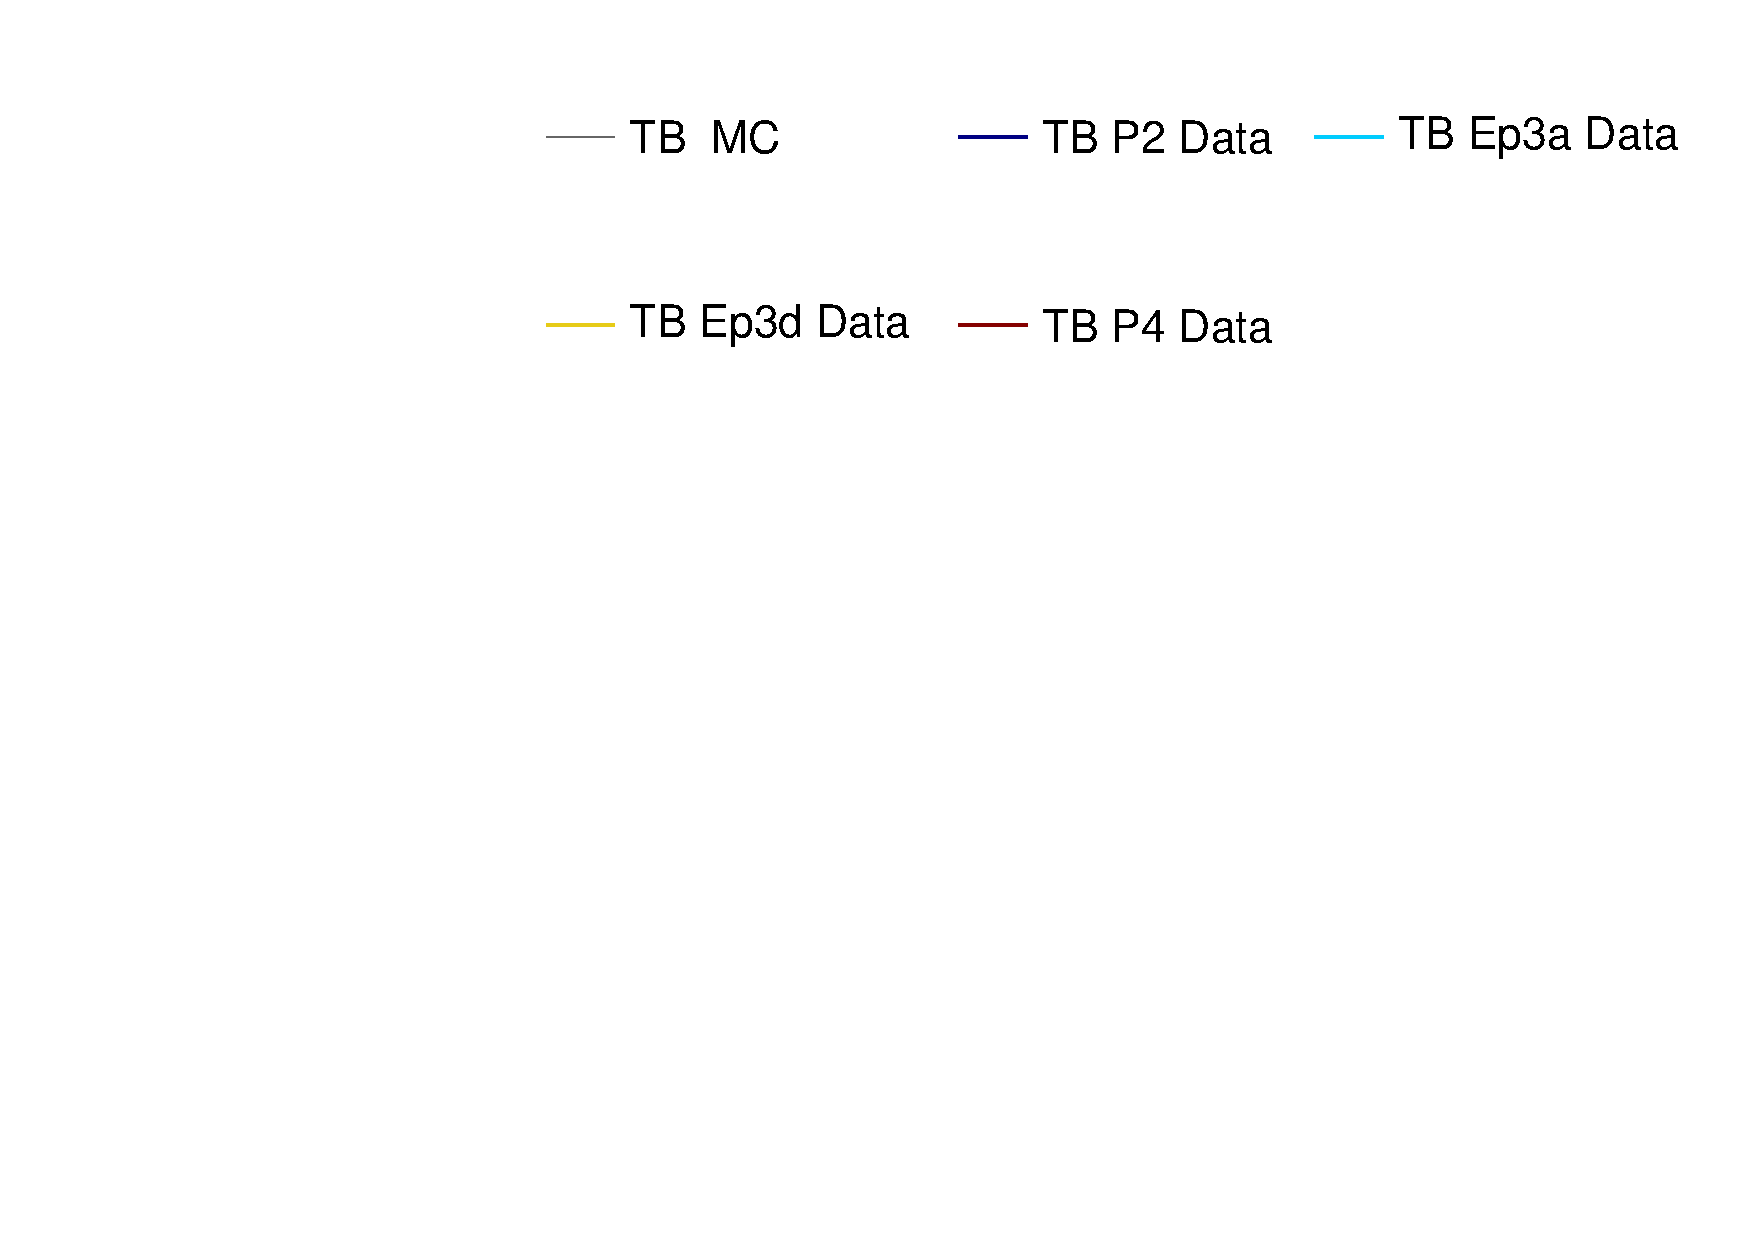
\includegraphics[height=0.2\linewidth]{essentialsec_tb/legend.pdf}
  \end{subfigure}
  \vspace*{2mm}

  \begin{subfigure}{0.5\textwidth}
    \includegraphics[width=\linewidth]{essentialsec_tb/pecm_cell_x.pdf}
  \end{subfigure}
  \begin{subfigure}{0.5\textwidth}
    \includegraphics[width=\linewidth]{essentialsec_tb/pecm_cell_y.pdf}
  \end{subfigure}
  \begin{subfigure}{0.5\textwidth}
    \includegraphics[width=\linewidth]{essentialsec_tb/pecorrcm_cell_x.pdf}
  \end{subfigure}
  \begin{subfigure}{0.5\textwidth}
    \includegraphics[width=\linewidth]{essentialsec_tb/pecorrcm_cell_y.pdf}
  \end{subfigure}
  \caption{...}
  \label{figAbsCalibCell1}
\end{figure}

\begin{figure}[h!]
  \begin{subfigure}{\textwidth}
  \centering
    \includegraphics[height=0.2\linewidth]{essentialsec_tb/legend.pdf}
  \end{subfigure}
  \vspace*{2mm}

  \begin{subfigure}{0.5\textwidth}
    \includegraphics[width=\linewidth]{essentialsec_tb/pe_cell_x.pdf}
  \end{subfigure}
  \begin{subfigure}{0.5\textwidth}
    \includegraphics[width=\linewidth]{essentialsec_tb/pe_cell_y.pdf}
  \end{subfigure}
  \begin{subfigure}{0.5\textwidth}
    \includegraphics[width=\linewidth]{essentialsec_tb/pecorr_cell_x.pdf}
  \end{subfigure}
  \begin{subfigure}{0.5\textwidth}
    \includegraphics[width=\linewidth]{essentialsec_tb/pecorr_cell_y.pdf}
  \end{subfigure}
  \begin{subfigure}{0.5\textwidth}
    \includegraphics[width=\linewidth]{essentialsec_tb/cm_cell_x.pdf}
  \end{subfigure}
  \begin{subfigure}{0.5\textwidth}
    \includegraphics[width=\linewidth]{essentialsec_tb/cm_cell_y.pdf}
  \end{subfigure}
  \caption{...}
  \label{figAbsCalibCell2}
\end{figure}

\begin{figure}[h!]
  \begin{subfigure}{\textwidth}
  \centering
    \includegraphics[height=0.2\linewidth]{essentialsec_tb/legend.pdf}
  \end{subfigure}
  \vspace*{2mm}

  \begin{subfigure}{0.5\textwidth}
    \includegraphics[width=\linewidth]{essentialsec_tb/pecm_plane_x.pdf}
  \end{subfigure}
  \begin{subfigure}{0.5\textwidth}
    \includegraphics[width=\linewidth]{essentialsec_tb/pecm_plane_y.pdf}
  \end{subfigure}
  \begin{subfigure}{0.5\textwidth}
    \includegraphics[width=\linewidth]{essentialsec_tb/pecorrcm_plane_x.pdf}
  \end{subfigure}
  \begin{subfigure}{0.5\textwidth}
    \includegraphics[width=\linewidth]{essentialsec_tb/pecorrcm_plane_y.pdf}
  \end{subfigure}
  \caption{...}
  \label{figAbsCalibPlane1}
\end{figure}

\begin{figure}[h!]
  \begin{subfigure}{\textwidth}
  \centering
    \includegraphics[height=0.2\linewidth]{essentialsec_tb/legend.pdf}
  \end{subfigure}
  \vspace*{2mm}

  \begin{subfigure}{0.5\textwidth}
    \includegraphics[width=\linewidth]{essentialsec_tb/pe_plane_x.pdf}
  \end{subfigure}
  \begin{subfigure}{0.5\textwidth}
    \includegraphics[width=\linewidth]{essentialsec_tb/pe_plane_y.pdf}
  \end{subfigure}
  \begin{subfigure}{0.5\textwidth}
    \includegraphics[width=\linewidth]{essentialsec_tb/pecorr_plane_x.pdf}
  \end{subfigure}
  \begin{subfigure}{0.5\textwidth}
    \includegraphics[width=\linewidth]{essentialsec_tb/pecorr_plane_y.pdf}
  \end{subfigure}
  \begin{subfigure}{0.5\textwidth}
    \includegraphics[width=\linewidth]{essentialsec_tb/cm_plane_x.pdf}
  \end{subfigure}
  \begin{subfigure}{0.5\textwidth}
    \includegraphics[width=\linewidth]{essentialsec_tb/cm_plane_y.pdf}
  \end{subfigure}
  \caption{...}
  \label{figAbsCalibPlane2}
\end{figure}

\begin{figure}[h!]
  \begin{subfigure}{\textwidth}
  \centering
    \includegraphics[height=0.2\linewidth]{essentialsec_tb/legend.pdf}
  \end{subfigure}
  \vspace*{2mm}

  \begin{subfigure}{0.5\textwidth}
    \includegraphics[width=\linewidth]{PlotsAngularDistribution/pecm_cosx_x.pdf}
  \end{subfigure}
  \begin{subfigure}{0.5\textwidth}
    \includegraphics[width=\linewidth]{PlotsAngularDistribution/pecm_cosx_y.pdf}
  \end{subfigure}
  \begin{subfigure}{0.5\textwidth}
    \includegraphics[width=\linewidth]{PlotsAngularDistribution/pecorrcm_cosx_x.pdf}
  \end{subfigure}
  \begin{subfigure}{0.5\textwidth}
    \includegraphics[width=\linewidth]{PlotsAngularDistribution/pecorrcm_cosx_y.pdf}
  \end{subfigure}
  \caption{...}
  \label{figAbsCalibCosX1}
\end{figure}

\begin{figure}[h!]
  \begin{subfigure}{\textwidth}
  \centering
    \includegraphics[height=0.2\linewidth]{essentialsec_tb/legend.pdf}
  \end{subfigure}
  \vspace*{2mm}

  \begin{subfigure}{0.5\textwidth}
    \includegraphics[width=\linewidth]{PlotsAngularDistribution/pe_cosx_x.pdf}
  \end{subfigure}
  \begin{subfigure}{0.5\textwidth}
    \includegraphics[width=\linewidth]{PlotsAngularDistribution/pe_cosx_y.pdf}
  \end{subfigure}
  \begin{subfigure}{0.5\textwidth}
    \includegraphics[width=\linewidth]{PlotsAngularDistribution/pecorr_cosx_x.pdf}
  \end{subfigure}
  \begin{subfigure}{0.5\textwidth}
    \includegraphics[width=\linewidth]{PlotsAngularDistribution/pecorr_cosx_y.pdf}
  \end{subfigure}
  \begin{subfigure}{0.5\textwidth}
    \includegraphics[width=\linewidth]{PlotsAngularDistribution/cm_cosx_x.pdf}
  \end{subfigure}
  \begin{subfigure}{0.5\textwidth}
    \includegraphics[width=\linewidth]{PlotsAngularDistribution/cm_cosx_y.pdf}
  \end{subfigure}
  \caption{...}
  \label{figAbsCalibCosX2}
\end{figure}

\begin{figure}[h!]
  \begin{subfigure}{\textwidth}
  \centering
    \includegraphics[height=0.2\linewidth]{essentialsec_tb/legend.pdf}
  \end{subfigure}
  \vspace*{2mm}
  
  \begin{subfigure}{0.5\textwidth}
    \includegraphics[width=\linewidth]{PlotsAngularDistribution/pecm_cosy_x.pdf}
  \end{subfigure}
  \begin{subfigure}{0.5\textwidth}
    \includegraphics[width=\linewidth]{PlotsAngularDistribution/pecm_cosy_y.pdf}
  \end{subfigure}
  \begin{subfigure}{0.5\textwidth}
    \includegraphics[width=\linewidth]{PlotsAngularDistribution/pecorrcm_cosy_x.pdf}
  \end{subfigure}
  \begin{subfigure}{0.5\textwidth}
    \includegraphics[width=\linewidth]{PlotsAngularDistribution/pecorrcm_cosy_y.pdf}
  \end{subfigure}
  \caption{...}
  \label{figAbsCalibCosY1}
\end{figure}

\begin{figure}[h!]
  \begin{subfigure}{\textwidth}
  \centering
    \includegraphics[height=0.2\linewidth]{essentialsec_tb/legend.pdf}
  \end{subfigure}
  \vspace*{2mm}

  \begin{subfigure}{0.5\textwidth}
    \includegraphics[width=\linewidth]{PlotsAngularDistribution/pe_cosy_x.pdf}
  \end{subfigure}
  \begin{subfigure}{0.5\textwidth}
    \includegraphics[width=\linewidth]{PlotsAngularDistribution/pe_cosy_y.pdf}
  \end{subfigure}
  \begin{subfigure}{0.5\textwidth}
    \includegraphics[width=\linewidth]{PlotsAngularDistribution/pecorr_cosy_x.pdf}
  \end{subfigure}
  \begin{subfigure}{0.5\textwidth}
    \includegraphics[width=\linewidth]{PlotsAngularDistribution/pecorr_cosy_y.pdf}
  \end{subfigure}
  \begin{subfigure}{0.5\textwidth}
    \includegraphics[width=\linewidth]{PlotsAngularDistribution/cm_cosy_x.pdf}
  \end{subfigure}
  \begin{subfigure}{0.5\textwidth}
    \includegraphics[width=\linewidth]{PlotsAngularDistribution/cm_cosy_y.pdf}
  \end{subfigure}
  \caption{...}
  \label{figAbsCalibCosY2}
\end{figure}

\begin{figure}[h!]
  \begin{subfigure}{\textwidth}
  \centering
    \includegraphics[height=0.2\linewidth]{essentialsec_tb/legend.pdf}
  \end{subfigure}
  \vspace*{2mm}
  
  \begin{subfigure}{0.5\textwidth}
    \includegraphics[width=\linewidth]{PlotsAngularDistribution/pecm_cosz_x.pdf}
  \end{subfigure}
  \begin{subfigure}{0.5\textwidth}
    \includegraphics[width=\linewidth]{PlotsAngularDistribution/pecm_cosz_y.pdf}
  \end{subfigure}
  \begin{subfigure}{0.5\textwidth}
    \includegraphics[width=\linewidth]{PlotsAngularDistribution/pecorrcm_cosz_x.pdf}
  \end{subfigure}
  \begin{subfigure}{0.5\textwidth}
    \includegraphics[width=\linewidth]{PlotsAngularDistribution/pecorrcm_cosz_y.pdf}
  \end{subfigure}
  \caption{...}
  \label{figAbsCalibCosZ1}
\end{figure}

\begin{figure}[h!]
  \begin{subfigure}{\textwidth}
    \centering
    \includegraphics[height=0.2\linewidth]{essentialsec_tb/legend.pdf}
  \end{subfigure}
  \vspace*{2mm}
  
  \begin{subfigure}{0.5\textwidth}
    \includegraphics[width=\linewidth]{PlotsAngularDistribution/pe_cosz_x.pdf}
  \end{subfigure}
  \begin{subfigure}{0.5\textwidth}
    \includegraphics[width=\linewidth]{PlotsAngularDistribution/pe_cosz_y.pdf}
  \end{subfigure}
  \begin{subfigure}{0.5\textwidth}
    \includegraphics[width=\linewidth]{PlotsAngularDistribution/pecorr_cosz_x.pdf}
  \end{subfigure}
  \begin{subfigure}{0.5\textwidth}
    \includegraphics[width=\linewidth]{PlotsAngularDistribution/pecorr_cosz_y.pdf}
  \end{subfigure}
  \begin{subfigure}{0.5\textwidth}
    \includegraphics[width=\linewidth]{PlotsAngularDistribution/cm_cosz_x.pdf}
  \end{subfigure}
  \begin{subfigure}{0.5\textwidth}
    \includegraphics[width=\linewidth]{PlotsAngularDistribution/cm_cosz_y.pdf}
  \end{subfigure}
  \caption{...}
  \label{figAbsCalibCosZ2}
\end{figure}

\subsection{Drift in TB data}

\begin{figure}[h!]
  \begin{subfigure}{\textwidth}
    \centering
    \includegraphics[height=0.2\linewidth]{essentialsec_tb/legend.pdf}
  \end{subfigure}
  \vspace*{2mm}
  
  \begin{subfigure}{0.5\textwidth}
    \includegraphics[width=\linewidth]{driftsec_tb/pecm_time_x.pdf}
  \end{subfigure}
  \begin{subfigure}{0.5\textwidth}
    \includegraphics[width=\linewidth]{driftsec_tb/pecm_time_y.pdf}
  \end{subfigure}
  \begin{subfigure}{0.5\textwidth}
    \includegraphics[width=\linewidth]{driftsec_tb/pecorrcm_time_x.pdf}
  \end{subfigure}
  \begin{subfigure}{0.5\textwidth}
    \includegraphics[width=\linewidth]{driftsec_tb/pecorrcm_time_y.pdf}
  \end{subfigure}
  \caption{...}
  \label{figAbsCalibDrift1}
\end{figure}

\begin{figure}[h!]
  \begin{subfigure}{\textwidth}
    \centering
    \includegraphics[height=0.2\linewidth]{essentialsec_tb/legend.pdf}
  \end{subfigure}
  \vspace*{2mm}
  
  \begin{subfigure}{0.5\textwidth}
    \includegraphics[width=\linewidth]{driftsec_tb/pe_time_x.pdf}
  \end{subfigure}
  \begin{subfigure}{0.5\textwidth}
    \includegraphics[width=\linewidth]{driftsec_tb/pe_time_y.pdf}
  \end{subfigure}
  \begin{subfigure}{0.5\textwidth}
    \includegraphics[width=\linewidth]{driftsec_tb/pecorr_time_x.pdf}
  \end{subfigure}
  \begin{subfigure}{0.5\textwidth}
    \includegraphics[width=\linewidth]{driftsec_tb/pecorr_time_y.pdf}
  \end{subfigure}
  \begin{subfigure}{0.5\textwidth}
    \includegraphics[width=\linewidth]{driftsec_tb/cm_time_x.pdf}
  \end{subfigure}
  \begin{subfigure}{0.5\textwidth}
    \includegraphics[width=\linewidth]{driftsec_tb/cm_time_y.pdf}
  \end{subfigure}
  \caption{...}
  \label{figAbsCalibDrift2}
\end{figure}

\subsection{Results}
Table of final results.
Final CSVs are locate in the \path{/nova/ana/testbeam/calibration} and they have been included in the vXX.XX calibration tag.

Plots of absolute calibration results

\subsection{Validation}
Comparisons with older version of calibration and maybe with the FD and ND

\end{document}